\documentclass[twoside]{book}

% Packages required by doxygen
\usepackage{fixltx2e}
\usepackage{calc}
\usepackage{doxygen}
\usepackage[export]{adjustbox} % also loads graphicx
\usepackage{graphicx}
\usepackage[utf8]{inputenc}
\usepackage{makeidx}
\usepackage{multicol}
\usepackage{multirow}
\PassOptionsToPackage{warn}{textcomp}
\usepackage{textcomp}
\usepackage[nointegrals]{wasysym}
\usepackage[table]{xcolor}

% Font selection
\usepackage[T1]{fontenc}
\usepackage[scaled=.90]{helvet}
\usepackage{courier}
\usepackage{amssymb}
\usepackage{sectsty}
\renewcommand{\familydefault}{\sfdefault}
\allsectionsfont{%
  \fontseries{bc}\selectfont%
  \color{darkgray}%
}
\renewcommand{\DoxyLabelFont}{%
  \fontseries{bc}\selectfont%
  \color{darkgray}%
}
\newcommand{\+}{\discretionary{\mbox{\scriptsize$\hookleftarrow$}}{}{}}

% Page & text layout
\usepackage{geometry}
\geometry{%
  a4paper,%
  top=2.5cm,%
  bottom=2.5cm,%
  left=2.5cm,%
  right=2.5cm%
}
\tolerance=750
\hfuzz=15pt
\hbadness=750
\setlength{\emergencystretch}{15pt}
\setlength{\parindent}{0cm}
\setlength{\parskip}{3ex plus 2ex minus 2ex}
\makeatletter
\renewcommand{\paragraph}{%
  \@startsection{paragraph}{4}{0ex}{-1.0ex}{1.0ex}{%
    \normalfont\normalsize\bfseries\SS@parafont%
  }%
}
\renewcommand{\subparagraph}{%
  \@startsection{subparagraph}{5}{0ex}{-1.0ex}{1.0ex}{%
    \normalfont\normalsize\bfseries\SS@subparafont%
  }%
}
\makeatother

% Headers & footers
\usepackage{fancyhdr}
\pagestyle{fancyplain}
\fancyhead[LE]{\fancyplain{}{\bfseries\thepage}}
\fancyhead[CE]{\fancyplain{}{}}
\fancyhead[RE]{\fancyplain{}{\bfseries\leftmark}}
\fancyhead[LO]{\fancyplain{}{\bfseries\rightmark}}
\fancyhead[CO]{\fancyplain{}{}}
\fancyhead[RO]{\fancyplain{}{\bfseries\thepage}}
\fancyfoot[LE]{\fancyplain{}{}}
\fancyfoot[CE]{\fancyplain{}{}}
\fancyfoot[RE]{\fancyplain{}{\bfseries\scriptsize Generated by Doxygen }}
\fancyfoot[LO]{\fancyplain{}{\bfseries\scriptsize Generated by Doxygen }}
\fancyfoot[CO]{\fancyplain{}{}}
\fancyfoot[RO]{\fancyplain{}{}}
\renewcommand{\footrulewidth}{0.4pt}
\renewcommand{\chaptermark}[1]{%
  \markboth{#1}{}%
}
\renewcommand{\sectionmark}[1]{%
  \markright{\thesection\ #1}%
}

% Indices & bibliography
\usepackage{natbib}
\usepackage[titles]{tocloft}
\setcounter{tocdepth}{3}
\setcounter{secnumdepth}{5}
\makeindex

% Hyperlinks (required, but should be loaded last)
\usepackage{ifpdf}
\ifpdf
  \usepackage[pdftex,pagebackref=true]{hyperref}
\else
  \usepackage[ps2pdf,pagebackref=true]{hyperref}
\fi
\hypersetup{%
  colorlinks=true,%
  linkcolor=blue,%
  citecolor=blue,%
  unicode%
}

% Custom commands
\newcommand{\clearemptydoublepage}{%
  \newpage{\pagestyle{empty}\cleardoublepage}%
}

\usepackage{caption}
\captionsetup{labelsep=space,justification=centering,font={bf},singlelinecheck=off,skip=4pt,position=top}

%===== C O N T E N T S =====

\begin{document}

% Titlepage & ToC
\hypersetup{pageanchor=false,
             bookmarksnumbered=true,
             pdfencoding=unicode
            }
\pagenumbering{alph}
\begin{titlepage}
\vspace*{7cm}
\begin{center}%
{\Large Z\+IA }\\
\vspace*{1cm}
{\large Generated by Doxygen 1.8.13}\\
\end{center}
\end{titlepage}
\clearemptydoublepage
\pagenumbering{roman}
\tableofcontents
\clearemptydoublepage
\pagenumbering{arabic}
\hypersetup{pageanchor=true}

%--- Begin generated contents ---
\chapter{Z\+IA}
\label{md_README}
\Hypertarget{md_README}
Insert description

\subsection*{Installation}

Install \href{https://conan.io/downloads.html}{\tt Conan} 📦 and \href{https://cmake.org/download/}{\tt C\+Make} 🏭 on your machine.

✔️ Check if you have a valid C++ compiler (eg. G\+CC, M\+S\+VC, ...)

\#\#\# Windows 
\begin{DoxyCode}
build
\end{DoxyCode}
 ➡ Next open the .snl solution with Visual Studio and build her.

\#\#\# Linux 
\begin{DoxyCode}
./build.sh
\end{DoxyCode}


The both binary (server, client) can be found in \char`\"{}build/bin/\char`\"{} folder 📁.

\subsection*{Usage}

Insert usage

\subsection*{License}

\href{https://choosealicense.com/licenses/mit/}{\tt M\+IT} 
\chapter{Hierarchical Index}
\section{Class Hierarchy}
This inheritance list is sorted roughly, but not completely, alphabetically\+:\begin{DoxyCompactList}
\item \contentsline{section}{module\+:\+:Api}{\pageref{structmodule_1_1Api}}{}
\begin{DoxyCompactList}
\item \contentsline{section}{module\+:\+:File}{\pageref{classmodule_1_1File}}{}
\item \contentsline{section}{module\+:\+:Php}{\pageref{classmodule_1_1Php}}{}
\item \contentsline{section}{module\+:\+:Proxy}{\pageref{classmodule_1_1Proxy}}{}
\end{DoxyCompactList}
\item \contentsline{section}{ihm\+:\+:Cmd\+Line}{\pageref{classihm_1_1CmdLine}}{}
\item \contentsline{section}{ihm\+:\+:command\+\_\+t}{\pageref{structihm_1_1command__t}}{}
\item \contentsline{section}{core\+:\+:Configurations}{\pageref{classcore_1_1Configurations}}{}
\item enable\+\_\+shared\+\_\+from\+\_\+this\begin{DoxyCompactList}
\item \contentsline{section}{net\+:\+:Boost\+Network\+Client}{\pageref{classnet_1_1BoostNetworkClient}}{}
\end{DoxyCompactList}
\item \contentsline{section}{http\+:\+:I\+Basic\+Object}{\pageref{structhttp_1_1IBasicObject}}{}
\begin{DoxyCompactList}
\item \contentsline{section}{http\+:\+:I\+Request}{\pageref{structhttp_1_1IRequest}}{}
\begin{DoxyCompactList}
\item \contentsline{section}{Http\+Request}{\pageref{classHttpRequest}}{}
\end{DoxyCompactList}
\item \contentsline{section}{http\+:\+:I\+Response}{\pageref{structhttp_1_1IResponse}}{}
\begin{DoxyCompactList}
\item \contentsline{section}{Http\+Response}{\pageref{classHttpResponse}}{}
\end{DoxyCompactList}
\end{DoxyCompactList}
\item \contentsline{section}{net\+:\+:I\+Client}{\pageref{structnet_1_1IClient}}{}
\begin{DoxyCompactList}
\item \contentsline{section}{Fake\+Client}{\pageref{classFakeClient}}{}
\item \contentsline{section}{Fake\+Client}{\pageref{classFakeClient}}{}
\item \contentsline{section}{Fake\+Client}{\pageref{classFakeClient}}{}
\item \contentsline{section}{net\+:\+:Boost\+Network\+Client}{\pageref{classnet_1_1BoostNetworkClient}}{}
\end{DoxyCompactList}
\item \contentsline{section}{I\+Config\+Node}{\pageref{classIConfigNode}}{}
\begin{DoxyCompactList}
\item \contentsline{section}{yconf\+:\+:Config\+Node}{\pageref{classyconf_1_1ConfigNode}}{}
\end{DoxyCompactList}
\item \contentsline{section}{net\+:\+:I\+Network\+Server}{\pageref{classnet_1_1INetworkServer}}{}
\begin{DoxyCompactList}
\item \contentsline{section}{net\+:\+:Boost\+Network\+Server}{\pageref{classnet_1_1BoostNetworkServer}}{}
\end{DoxyCompactList}
\item \contentsline{section}{core\+:\+:Listeners\+Control}{\pageref{classcore_1_1ListenersControl}}{}
\item \contentsline{section}{Module}{\pageref{classModule}}{}
\item \contentsline{section}{core\+:\+:config\+:\+:Module}{\pageref{classcore_1_1config_1_1Module}}{}
\item \contentsline{section}{core\+:\+:config\+:\+:Modules\+Container}{\pageref{classcore_1_1config_1_1ModulesContainer}}{}
\begin{DoxyCompactList}
\item \contentsline{section}{core\+:\+:config\+:\+:Host}{\pageref{classcore_1_1config_1_1Host}}{}
\item \contentsline{section}{core\+:\+:config\+:\+:Route}{\pageref{classcore_1_1config_1_1Route}}{}
\end{DoxyCompactList}
\item \contentsline{section}{net\+:\+:Network\+Manager}{\pageref{classnet_1_1NetworkManager}}{}
\item \contentsline{section}{Redirector}{\pageref{classRedirector}}{}
\end{DoxyCompactList}

\chapter{Class Index}
\section{Class List}
Here are the classes, structs, unions and interfaces with brief descriptions\+:\begin{DoxyCompactList}
\item\contentsline{section}{\hyperlink{structmodule_1_1Api}{module\+::\+Api} }{\pageref{structmodule_1_1Api}}{}
\item\contentsline{section}{\hyperlink{classnet_1_1BoostNetworkClient}{net\+::\+Boost\+Network\+Client} }{\pageref{classnet_1_1BoostNetworkClient}}{}
\item\contentsline{section}{\hyperlink{classnet_1_1BoostNetworkServer}{net\+::\+Boost\+Network\+Server} }{\pageref{classnet_1_1BoostNetworkServer}}{}
\item\contentsline{section}{\hyperlink{classihm_1_1CmdLine}{ihm\+::\+Cmd\+Line} \\*Interact with the user by tokenized string }{\pageref{classihm_1_1CmdLine}}{}
\item\contentsline{section}{\hyperlink{structihm_1_1command__t}{ihm\+::command\+\_\+t} }{\pageref{structihm_1_1command__t}}{}
\item\contentsline{section}{\hyperlink{classyconf_1_1ConfigNode}{yconf\+::\+Config\+Node} }{\pageref{classyconf_1_1ConfigNode}}{}
\item\contentsline{section}{\hyperlink{classcore_1_1Configurations}{core\+::\+Configurations} }{\pageref{classcore_1_1Configurations}}{}
\item\contentsline{section}{\hyperlink{classFakeClient}{Fake\+Client} }{\pageref{classFakeClient}}{}
\item\contentsline{section}{\hyperlink{classmodule_1_1File}{module\+::\+File} }{\pageref{classmodule_1_1File}}{}
\item\contentsline{section}{\hyperlink{classcore_1_1config_1_1Host}{core\+::config\+::\+Host} }{\pageref{classcore_1_1config_1_1Host}}{}
\item\contentsline{section}{\hyperlink{classHttpRequest}{Http\+Request} }{\pageref{classHttpRequest}}{}
\item\contentsline{section}{\hyperlink{classHttpResponse}{Http\+Response} }{\pageref{classHttpResponse}}{}
\item\contentsline{section}{\hyperlink{structhttp_1_1IBasicObject}{http\+::\+I\+Basic\+Object} \\*Http\+::\+I\+Basic\+Object is a interface that describe same object in a http request / response }{\pageref{structhttp_1_1IBasicObject}}{}
\item\contentsline{section}{\hyperlink{structnet_1_1IClient}{net\+::\+I\+Client} }{\pageref{structnet_1_1IClient}}{}
\item\contentsline{section}{\hyperlink{classIConfigNode}{I\+Config\+Node} }{\pageref{classIConfigNode}}{}
\item\contentsline{section}{\hyperlink{classnet_1_1INetworkServer}{net\+::\+I\+Network\+Server} }{\pageref{classnet_1_1INetworkServer}}{}
\item\contentsline{section}{\hyperlink{structhttp_1_1IRequest}{http\+::\+I\+Request} \\*Http\+::\+I\+Request is a interface that encapsulates a http request }{\pageref{structhttp_1_1IRequest}}{}
\item\contentsline{section}{\hyperlink{structhttp_1_1IResponse}{http\+::\+I\+Response} \\*Http\+::\+I\+Response is a interface that encapsulates a http response }{\pageref{structhttp_1_1IResponse}}{}
\item\contentsline{section}{\hyperlink{classcore_1_1ListenersControl}{core\+::\+Listeners\+Control} }{\pageref{classcore_1_1ListenersControl}}{}
\item\contentsline{section}{\hyperlink{classModule}{Module} \\*Loads module from dynamic library }{\pageref{classModule}}{}
\item\contentsline{section}{\hyperlink{classcore_1_1config_1_1Module}{core\+::config\+::\+Module} }{\pageref{classcore_1_1config_1_1Module}}{}
\item\contentsline{section}{\hyperlink{classcore_1_1config_1_1ModulesContainer}{core\+::config\+::\+Modules\+Container} }{\pageref{classcore_1_1config_1_1ModulesContainer}}{}
\item\contentsline{section}{\hyperlink{classnet_1_1NetworkManager}{net\+::\+Network\+Manager} }{\pageref{classnet_1_1NetworkManager}}{}
\item\contentsline{section}{\hyperlink{classmodule_1_1Php}{module\+::\+Php} }{\pageref{classmodule_1_1Php}}{}
\item\contentsline{section}{\hyperlink{classmodule_1_1Proxy}{module\+::\+Proxy} }{\pageref{classmodule_1_1Proxy}}{}
\item\contentsline{section}{\hyperlink{classRedirector}{Redirector} \\*Redirect ostream to get their content }{\pageref{classRedirector}}{}
\item\contentsline{section}{\hyperlink{classcore_1_1config_1_1Route}{core\+::config\+::\+Route} }{\pageref{classcore_1_1config_1_1Route}}{}
\end{DoxyCompactList}

\chapter{File Index}
\section{File List}
Here is a list of all documented files with brief descriptions\+:\begin{DoxyCompactList}
\item\contentsline{section}{inc/{\bfseries I\+Config\+Node.\+hpp} }{\pageref{IConfigNode_8hpp}}{}
\item\contentsline{section}{inc/\+Core/\+Configs/\hyperlink{Configurations_8hpp}{Configurations.\+hpp} }{\pageref{Configurations_8hpp}}{}
\item\contentsline{section}{inc/\+Core/\+Configs/\hyperlink{Host_8hpp}{Host.\+hpp} }{\pageref{Host_8hpp}}{}
\item\contentsline{section}{inc/\+Core/\+Configs/\hyperlink{Modules_8hpp}{Modules.\+hpp} }{\pageref{Modules_8hpp}}{}
\item\contentsline{section}{inc/\+Core/\+Configs/\hyperlink{ModulesContainer_8hpp}{Modules\+Container.\+hpp} }{\pageref{ModulesContainer_8hpp}}{}
\item\contentsline{section}{inc/\+Core/\+Configs/\hyperlink{Route_8hpp}{Route.\+hpp} }{\pageref{Route_8hpp}}{}
\item\contentsline{section}{inc/\+Core/\+Http/{\bfseries Http\+Request.\+hpp} }{\pageref{HttpRequest_8hpp}}{}
\item\contentsline{section}{inc/\+Core/\+Http/{\bfseries Http\+Response.\+hpp} }{\pageref{HttpResponse_8hpp}}{}
\item\contentsline{section}{inc/\+Core/\+Http/api/{\bfseries I\+Basic\+Object.\+hpp} }{\pageref{IBasicObject_8hpp}}{}
\item\contentsline{section}{inc/\+Core/\+Http/api/{\bfseries I\+Request.\+hpp} }{\pageref{IRequest_8hpp}}{}
\item\contentsline{section}{inc/\+Core/\+Http/api/{\bfseries I\+Response.\+hpp} }{\pageref{IResponse_8hpp}}{}
\item\contentsline{section}{inc/\+Core/\+Listeners/{\bfseries Listeners\+Control.\+hpp} }{\pageref{ListenersControl_8hpp}}{}
\item\contentsline{section}{inc/\+Core/\+Module/{\bfseries Module.\+hpp} }{\pageref{Module_8hpp}}{}
\item\contentsline{section}{inc/\+Core/\+Module/{\bfseries Module\+Api.\+hpp} }{\pageref{ModuleApi_8hpp}}{}
\item\contentsline{section}{inc/\+Ihm/\hyperlink{CmdLine_8hpp}{Cmd\+Line.\+hpp} }{\pageref{CmdLine_8hpp}}{}
\item\contentsline{section}{inc/\+Network/\hyperlink{BoostNetworkClient_8hpp}{Boost\+Network\+Client.\+hpp} \\*An boost asio instance to store and comunicate with a network client }{\pageref{BoostNetworkClient_8hpp}}{}
\item\contentsline{section}{inc/\+Network/\hyperlink{BoostNetworkServer_8hpp}{Boost\+Network\+Server.\+hpp} \\*Boost encapsulation of the server tcp }{\pageref{BoostNetworkServer_8hpp}}{}
\item\contentsline{section}{inc/\+Network/{\bfseries I\+Client.\+hpp} }{\pageref{IClient_8hpp}}{}
\item\contentsline{section}{inc/\+Network/\hyperlink{INetworkServer_8hpp}{I\+Network\+Server.\+hpp} \\*Server interface }{\pageref{INetworkServer_8hpp}}{}
\item\contentsline{section}{inc/\+Network/\hyperlink{NetworkManager_8hpp}{Network\+Manager.\+hpp} \\*Class to interract with network part and worker }{\pageref{NetworkManager_8hpp}}{}
\item\contentsline{section}{inc/yconf/{\bfseries Config\+Node.\+hpp} }{\pageref{ConfigNode_8hpp}}{}
\item\contentsline{section}{inc/yconf/{\bfseries Helper.\+hpp} }{\pageref{Helper_8hpp}}{}
\item\contentsline{section}{inc/yconf/{\bfseries util.\+hpp} }{\pageref{util_8hpp}}{}
\item\contentsline{section}{modules/\+File/\hyperlink{File_8cpp}{File.\+cpp} \\*An basic module who say hello at each requests }{\pageref{File_8cpp}}{}
\item\contentsline{section}{modules/\+File/\hyperlink{File_8hpp}{File.\+hpp} \\*An basic module who say hello at each requests }{\pageref{File_8hpp}}{}
\item\contentsline{section}{modules/\+Php/\hyperlink{Php_8cpp}{Php.\+cpp} }{\pageref{Php_8cpp}}{}
\item\contentsline{section}{modules/\+Php/\hyperlink{Php_8hpp}{Php.\+hpp} \\*An basic module who say hello at each requests }{\pageref{Php_8hpp}}{}
\item\contentsline{section}{modules/\+Proxy/\hyperlink{Proxy_8cpp}{Proxy.\+cpp} }{\pageref{Proxy_8cpp}}{}
\item\contentsline{section}{modules/\+Proxy/\hyperlink{Proxy_8hpp}{Proxy.\+hpp} }{\pageref{Proxy_8hpp}}{}
\item\contentsline{section}{src/\+Core/\+Configs/\hyperlink{Configurations_8cpp}{Configurations.\+cpp} }{\pageref{Configurations_8cpp}}{}
\item\contentsline{section}{src/\+Core/\+Configs/\hyperlink{Host_8cpp}{Host.\+cpp} }{\pageref{Host_8cpp}}{}
\item\contentsline{section}{src/\+Core/\+Configs/\hyperlink{ModulesContainer_8cpp}{Modules\+Container.\+cpp} }{\pageref{ModulesContainer_8cpp}}{}
\item\contentsline{section}{src/\+Core/\+Configs/\hyperlink{Route_8cpp}{Route.\+cpp} }{\pageref{Route_8cpp}}{}
\item\contentsline{section}{src/\+Core/\+Listeners/\hyperlink{ListenersControl_8cpp}{Listeners\+Control.\+cpp} }{\pageref{ListenersControl_8cpp}}{}
\item\contentsline{section}{src/\+Ihm/\hyperlink{CmdLine_8cpp}{Cmd\+Line.\+cpp} }{\pageref{CmdLine_8cpp}}{}
\item\contentsline{section}{src/\+Network/\hyperlink{NetworkManager_8cpp}{Network\+Manager.\+cpp} }{\pageref{NetworkManager_8cpp}}{}
\item\contentsline{section}{tests/\hyperlink{ModuleFile_8cpp}{Module\+File.\+cpp} }{\pageref{ModuleFile_8cpp}}{}
\item\contentsline{section}{tests/\hyperlink{ModulePhp_8cpp}{Module\+Php.\+cpp} }{\pageref{ModulePhp_8cpp}}{}
\item\contentsline{section}{tests/\hyperlink{ModuleProxy_8cpp}{Module\+Proxy.\+cpp} }{\pageref{ModuleProxy_8cpp}}{}
\item\contentsline{section}{tests/\hyperlink{Redirector_8hpp}{Redirector.\+hpp} }{\pageref{Redirector_8hpp}}{}
\item\contentsline{section}{tests/\hyperlink{RouteConf_8cpp}{Route\+Conf.\+cpp} }{\pageref{RouteConf_8cpp}}{}
\item\contentsline{section}{tests/\hyperlink{Server_8cpp}{Server.\+cpp} }{\pageref{Server_8cpp}}{}
\item\contentsline{section}{tests/\hyperlink{yml_8cpp}{yml.\+cpp} }{\pageref{yml_8cpp}}{}
\end{DoxyCompactList}

\chapter{Class Documentation}
\hypertarget{structmodule_1_1Api}{}\section{module\+:\+:Api Struct Reference}
\label{structmodule_1_1Api}\index{module\+::\+Api@{module\+::\+Api}}


Inheritance diagram for module\+:\+:Api\+:
\nopagebreak
\begin{figure}[H]
\begin{center}
\leavevmode
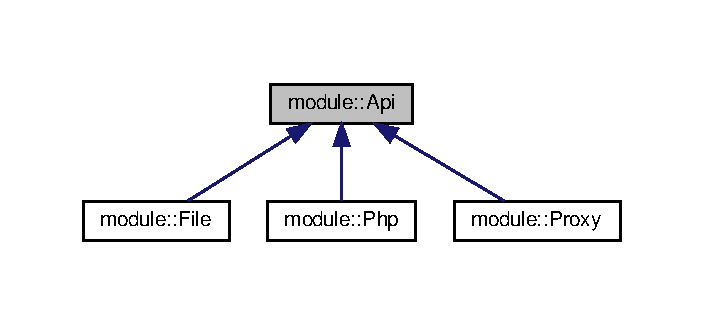
\includegraphics[width=338pt]{structmodule_1_1Api__inherit__graph}
\end{center}
\end{figure}
\subsection*{Public Member Functions}
\begin{DoxyCompactItemize}
\item 
\mbox{\Hypertarget{structmodule_1_1Api_a6c8d118958a709fc02b7253d39286327}\label{structmodule_1_1Api_a6c8d118958a709fc02b7253d39286327}} 
virtual \hyperlink{structmodule_1_1Api_a6c8d118958a709fc02b7253d39286327}{$\sim$\+Api} ()=default
\begin{DoxyCompactList}\small\item\em Default destructor. \end{DoxyCompactList}\item 
\mbox{\Hypertarget{structmodule_1_1Api_a183b56d5e35e77fa76d02ab27f55f742}\label{structmodule_1_1Api_a183b56d5e35e77fa76d02ab27f55f742}} 
virtual std\+::string \hyperlink{structmodule_1_1Api_a183b56d5e35e77fa76d02ab27f55f742}{name} () const noexcept=0
\begin{DoxyCompactList}\small\item\em Returns the module name. \end{DoxyCompactList}\item 
virtual bool \hyperlink{structmodule_1_1Api_aa83ddc92765200dd65f915498175c2be}{new\+Connection} (const \hyperlink{structnet_1_1IClient}{net\+::\+I\+Client} \&client) noexcept=0
\begin{DoxyCompactList}\small\item\em When a new client connects to the http server. \end{DoxyCompactList}\item 
virtual bool \hyperlink{structmodule_1_1Api_a8aa98bd4094fb13916e100509a948763}{disconnection} (const \hyperlink{structnet_1_1IClient}{net\+::\+I\+Client} \&client) noexcept=0
\begin{DoxyCompactList}\small\item\em When a client disconnects. \end{DoxyCompactList}\item 
\mbox{\Hypertarget{structmodule_1_1Api_a93b6a1380a8f0448ff5d06af8dbd03ca}\label{structmodule_1_1Api_a93b6a1380a8f0448ff5d06af8dbd03ca}} 
virtual bool \hyperlink{structmodule_1_1Api_a93b6a1380a8f0448ff5d06af8dbd03ca}{set\+Configurations} (Configs configs) noexcept=0
\begin{DoxyCompactList}\small\item\em Set the Global configs of the module. \end{DoxyCompactList}\item 
virtual bool \hyperlink{structmodule_1_1Api_ad8b56820e4f53bf65d34447184edef20}{after\+Receive} (const \hyperlink{structnet_1_1IClient}{net\+::\+I\+Client} \&client, std\+::string \&buffer) noexcept=0
\begin{DoxyCompactList}\small\item\em Just before the deserialization of the packet. \end{DoxyCompactList}\item 
virtual bool \hyperlink{structmodule_1_1Api_a291297e6d233e69b82c976e085f7c237}{after\+Unpacked} (const \hyperlink{structnet_1_1IClient}{net\+::\+I\+Client} \&client, \hyperlink{structhttp_1_1IRequest}{http\+::\+I\+Request} \&request) noexcept=0
\begin{DoxyCompactList}\small\item\em Call before the main behavior of the module. \end{DoxyCompactList}\item 
virtual bool \hyperlink{structmodule_1_1Api_afd1f5243a90811d06d96f725490bcba6}{execute} (const \hyperlink{structnet_1_1IClient}{net\+::\+I\+Client} \&client, \hyperlink{structhttp_1_1IRequest}{http\+::\+I\+Request} \&request, \hyperlink{structhttp_1_1IResponse}{http\+::\+I\+Response} \&response) noexcept=0
\begin{DoxyCompactList}\small\item\em This is the main behavior of the module. \end{DoxyCompactList}\item 
virtual bool \hyperlink{structmodule_1_1Api_a5293babe6b28a397b7a11f32da0a6f51}{before\+Packed} (const \hyperlink{structnet_1_1IClient}{net\+::\+I\+Client} \&client, \hyperlink{structhttp_1_1IResponse}{http\+::\+I\+Response} \&response) noexcept=0
\begin{DoxyCompactList}\small\item\em Just before the serialization of the response. \end{DoxyCompactList}\item 
virtual bool \hyperlink{structmodule_1_1Api_a71d1ada8bc5fc81fd71607315dd86185}{before\+Send} (const \hyperlink{structnet_1_1IClient}{net\+::\+I\+Client} \&client, std\+::string \&buffer) noexcept=0
\begin{DoxyCompactList}\small\item\em Just before packet delivery. \end{DoxyCompactList}\end{DoxyCompactItemize}


\subsection{Member Function Documentation}
\mbox{\Hypertarget{structmodule_1_1Api_ad8b56820e4f53bf65d34447184edef20}\label{structmodule_1_1Api_ad8b56820e4f53bf65d34447184edef20}} 
\index{module\+::\+Api@{module\+::\+Api}!after\+Receive@{after\+Receive}}
\index{after\+Receive@{after\+Receive}!module\+::\+Api@{module\+::\+Api}}
\subsubsection{\texorpdfstring{after\+Receive()}{afterReceive()}}
{\footnotesize\ttfamily virtual bool module\+::\+Api\+::after\+Receive (\begin{DoxyParamCaption}\item[{const \hyperlink{structnet_1_1IClient}{net\+::\+I\+Client} \&}]{client,  }\item[{std\+::string \&}]{buffer }\end{DoxyParamCaption})\hspace{0.3cm}{\ttfamily [pure virtual]}, {\ttfamily [noexcept]}}



Just before the deserialization of the packet. 

It can be useful to decrypt an tls packet 

Implemented in \hyperlink{classmodule_1_1Proxy_a0dbbd27ea29602830d770c5c550b1ee4}{module\+::\+Proxy}, \hyperlink{classmodule_1_1File_af37dc06c40ef291f3789ae4b00e628d7}{module\+::\+File}, and \hyperlink{classmodule_1_1Php_a553dd60d283baf309a9ba8ddb87681b8}{module\+::\+Php}.

\mbox{\Hypertarget{structmodule_1_1Api_a291297e6d233e69b82c976e085f7c237}\label{structmodule_1_1Api_a291297e6d233e69b82c976e085f7c237}} 
\index{module\+::\+Api@{module\+::\+Api}!after\+Unpacked@{after\+Unpacked}}
\index{after\+Unpacked@{after\+Unpacked}!module\+::\+Api@{module\+::\+Api}}
\subsubsection{\texorpdfstring{after\+Unpacked()}{afterUnpacked()}}
{\footnotesize\ttfamily virtual bool module\+::\+Api\+::after\+Unpacked (\begin{DoxyParamCaption}\item[{const \hyperlink{structnet_1_1IClient}{net\+::\+I\+Client} \&}]{client,  }\item[{\hyperlink{structhttp_1_1IRequest}{http\+::\+I\+Request} \&}]{request }\end{DoxyParamCaption})\hspace{0.3cm}{\ttfamily [pure virtual]}, {\ttfamily [noexcept]}}



Call before the main behavior of the module. 

It can be useful to decompresses a http body (gzip, ...) 

Implemented in \hyperlink{classmodule_1_1Proxy_a16524232b12bd03353c79bcda4bd8d15}{module\+::\+Proxy}, \hyperlink{classmodule_1_1File_a201c3c9c01df460e22f270c554937639}{module\+::\+File}, and \hyperlink{classmodule_1_1Php_ae3f23ea75718c51e0427fa2d13ab9755}{module\+::\+Php}.

\mbox{\Hypertarget{structmodule_1_1Api_a5293babe6b28a397b7a11f32da0a6f51}\label{structmodule_1_1Api_a5293babe6b28a397b7a11f32da0a6f51}} 
\index{module\+::\+Api@{module\+::\+Api}!before\+Packed@{before\+Packed}}
\index{before\+Packed@{before\+Packed}!module\+::\+Api@{module\+::\+Api}}
\subsubsection{\texorpdfstring{before\+Packed()}{beforePacked()}}
{\footnotesize\ttfamily virtual bool module\+::\+Api\+::before\+Packed (\begin{DoxyParamCaption}\item[{const \hyperlink{structnet_1_1IClient}{net\+::\+I\+Client} \&}]{client,  }\item[{\hyperlink{structhttp_1_1IResponse}{http\+::\+I\+Response} \&}]{response }\end{DoxyParamCaption})\hspace{0.3cm}{\ttfamily [pure virtual]}, {\ttfamily [noexcept]}}



Just before the serialization of the response. 

Useful if we need to add something in the packet or to compress it 

Implemented in \hyperlink{classmodule_1_1Proxy_a3b88487ecaaa856f319d78f2aa6358c1}{module\+::\+Proxy}, \hyperlink{classmodule_1_1File_ab2004b38d5dd63e0e19f358a3820477f}{module\+::\+File}, and \hyperlink{classmodule_1_1Php_a71b22ae01eedfd3406d01907cd7dc3d9}{module\+::\+Php}.

\mbox{\Hypertarget{structmodule_1_1Api_a71d1ada8bc5fc81fd71607315dd86185}\label{structmodule_1_1Api_a71d1ada8bc5fc81fd71607315dd86185}} 
\index{module\+::\+Api@{module\+::\+Api}!before\+Send@{before\+Send}}
\index{before\+Send@{before\+Send}!module\+::\+Api@{module\+::\+Api}}
\subsubsection{\texorpdfstring{before\+Send()}{beforeSend()}}
{\footnotesize\ttfamily virtual bool module\+::\+Api\+::before\+Send (\begin{DoxyParamCaption}\item[{const \hyperlink{structnet_1_1IClient}{net\+::\+I\+Client} \&}]{client,  }\item[{std\+::string \&}]{buffer }\end{DoxyParamCaption})\hspace{0.3cm}{\ttfamily [pure virtual]}, {\ttfamily [noexcept]}}



Just before packet delivery. 

Useful if we need to add something in the packet or to encrypt 

Implemented in \hyperlink{classmodule_1_1Proxy_a314d53ca09edbb7f2595cefb5c55771e}{module\+::\+Proxy}, \hyperlink{classmodule_1_1File_a13091749fbe954576d351e90e15581d7}{module\+::\+File}, and \hyperlink{classmodule_1_1Php_a9ba9768f149e9dbf3094d5cdb4967fc3}{module\+::\+Php}.

\mbox{\Hypertarget{structmodule_1_1Api_a8aa98bd4094fb13916e100509a948763}\label{structmodule_1_1Api_a8aa98bd4094fb13916e100509a948763}} 
\index{module\+::\+Api@{module\+::\+Api}!disconnection@{disconnection}}
\index{disconnection@{disconnection}!module\+::\+Api@{module\+::\+Api}}
\subsubsection{\texorpdfstring{disconnection()}{disconnection()}}
{\footnotesize\ttfamily virtual bool module\+::\+Api\+::disconnection (\begin{DoxyParamCaption}\item[{const \hyperlink{structnet_1_1IClient}{net\+::\+I\+Client} \&}]{client }\end{DoxyParamCaption})\hspace{0.3cm}{\ttfamily [pure virtual]}, {\ttfamily [noexcept]}}



When a client disconnects. 

To inform the module of the client\textquotesingle{}s disconnection 

Implemented in \hyperlink{classmodule_1_1Proxy_aa80f5772c7c4613060f4cf49f1fc00e4}{module\+::\+Proxy}, \hyperlink{classmodule_1_1File_a86bd2e04ae5946fb790342911b9e4454}{module\+::\+File}, and \hyperlink{classmodule_1_1Php_af828a98b73d3da6a53a64d4b3b3927c4}{module\+::\+Php}.

\mbox{\Hypertarget{structmodule_1_1Api_afd1f5243a90811d06d96f725490bcba6}\label{structmodule_1_1Api_afd1f5243a90811d06d96f725490bcba6}} 
\index{module\+::\+Api@{module\+::\+Api}!execute@{execute}}
\index{execute@{execute}!module\+::\+Api@{module\+::\+Api}}
\subsubsection{\texorpdfstring{execute()}{execute()}}
{\footnotesize\ttfamily virtual bool module\+::\+Api\+::execute (\begin{DoxyParamCaption}\item[{const \hyperlink{structnet_1_1IClient}{net\+::\+I\+Client} \&}]{client,  }\item[{\hyperlink{structhttp_1_1IRequest}{http\+::\+I\+Request} \&}]{request,  }\item[{\hyperlink{structhttp_1_1IResponse}{http\+::\+I\+Response} \&}]{response }\end{DoxyParamCaption})\hspace{0.3cm}{\ttfamily [pure virtual]}, {\ttfamily [noexcept]}}



This is the main behavior of the module. 

Reaction to the client\textquotesingle{}s request 

Implemented in \hyperlink{classmodule_1_1Proxy_a7a210c144da81f379a7ca6b7ef7914c8}{module\+::\+Proxy}, \hyperlink{classmodule_1_1File_a7fceec434dd7b735e08b01a5bd16625b}{module\+::\+File}, and \hyperlink{classmodule_1_1Php_aa73bfe086a0015a892f7d5687639aafb}{module\+::\+Php}.

\mbox{\Hypertarget{structmodule_1_1Api_aa83ddc92765200dd65f915498175c2be}\label{structmodule_1_1Api_aa83ddc92765200dd65f915498175c2be}} 
\index{module\+::\+Api@{module\+::\+Api}!new\+Connection@{new\+Connection}}
\index{new\+Connection@{new\+Connection}!module\+::\+Api@{module\+::\+Api}}
\subsubsection{\texorpdfstring{new\+Connection()}{newConnection()}}
{\footnotesize\ttfamily virtual bool module\+::\+Api\+::new\+Connection (\begin{DoxyParamCaption}\item[{const \hyperlink{structnet_1_1IClient}{net\+::\+I\+Client} \&}]{client }\end{DoxyParamCaption})\hspace{0.3cm}{\ttfamily [pure virtual]}, {\ttfamily [noexcept]}}



When a new client connects to the http server. 

It can be useful to store the id of the client to recognize him after 

Implemented in \hyperlink{classmodule_1_1Proxy_a92e33605f1164599922fa64d936f5b77}{module\+::\+Proxy}, \hyperlink{classmodule_1_1File_a369f5f98cfbc477e345b7372319737d7}{module\+::\+File}, and \hyperlink{classmodule_1_1Php_adc03ae040e0a938640bd4ba9a6eb2d3c}{module\+::\+Php}.



The documentation for this struct was generated from the following file\+:\begin{DoxyCompactItemize}
\item 
inc/\+Core/\+Module/Module\+Api.\+hpp\end{DoxyCompactItemize}

\hypertarget{classnet_1_1BoostNetworkClient}{}\section{net\+:\+:Boost\+Network\+Client Class Reference}
\label{classnet_1_1BoostNetworkClient}\index{net\+::\+Boost\+Network\+Client@{net\+::\+Boost\+Network\+Client}}


Inheritance diagram for net\+:\+:Boost\+Network\+Client\+:
\nopagebreak
\begin{figure}[H]
\begin{center}
\leavevmode
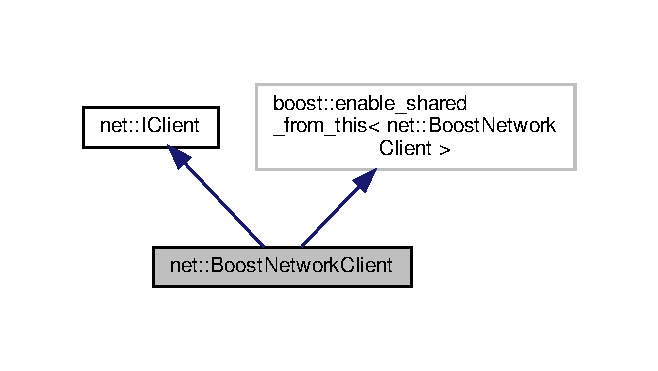
\includegraphics[width=316pt]{classnet_1_1BoostNetworkClient__inherit__graph}
\end{center}
\end{figure}


Collaboration diagram for net\+:\+:Boost\+Network\+Client\+:
\nopagebreak
\begin{figure}[H]
\begin{center}
\leavevmode
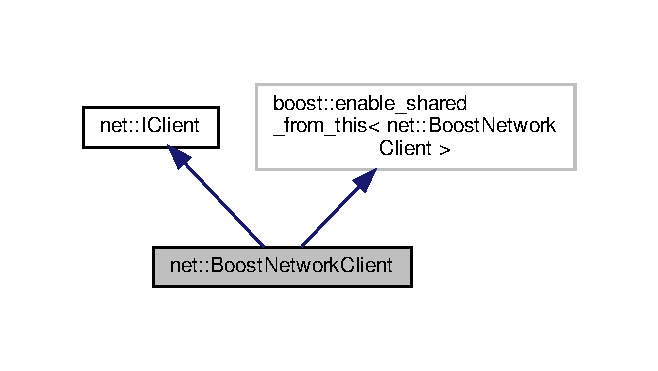
\includegraphics[width=316pt]{classnet_1_1BoostNetworkClient__coll__graph}
\end{center}
\end{figure}
\subsection*{Public Member Functions}
\begin{DoxyCompactItemize}
\item 
\mbox{\Hypertarget{classnet_1_1BoostNetworkClient_a832aefb3748593253acdc953c733476e}\label{classnet_1_1BoostNetworkClient_a832aefb3748593253acdc953c733476e}} 
{\bfseries Boost\+Network\+Client} (basic\+\_\+socket\+\_\+acceptor$<$ ip\+::tcp $>$ \&ec, \hyperlink{classnet_1_1NetworkManager}{Network\+Manager} \&network\+Manager)
\item 
bool \hyperlink{classnet_1_1BoostNetworkClient_af584270d274c31b315eba24effd86b46}{send} (const std\+::string \&data)
\begin{DoxyCompactList}\small\item\em Send \textquotesingle{}data\textquotesingle{} into a tcp packet to the client. \end{DoxyCompactList}\item 
\mbox{\Hypertarget{classnet_1_1BoostNetworkClient_a50ffb3f1689aebecf724d466894a25d1}\label{classnet_1_1BoostNetworkClient_a50ffb3f1689aebecf724d466894a25d1}} 
ip\+::tcp\+::socket \& {\bfseries get\+Socket} ()
\item 
\mbox{\Hypertarget{classnet_1_1BoostNetworkClient_ab552e0d494a73e0b6e97e4790642dab5}\label{classnet_1_1BoostNetworkClient_ab552e0d494a73e0b6e97e4790642dab5}} 
void {\bfseries bind\+Read} ()
\item 
\mbox{\Hypertarget{classnet_1_1BoostNetworkClient_a4228d9f794ae8e546e475852bdb495f7}\label{classnet_1_1BoostNetworkClient_a4228d9f794ae8e546e475852bdb495f7}} 
void {\bfseries disconnect} (const std\+::string \&message)
\item 
\mbox{\Hypertarget{classnet_1_1BoostNetworkClient_aa17822d06f0d13c4dfa44a32c877b31b}\label{classnet_1_1BoostNetworkClient_aa17822d06f0d13c4dfa44a32c877b31b}} 
void {\bfseries read\+Handler} (const boost\+::system\+::error\+\_\+code \&error, std\+::size\+\_\+t bytes\+\_\+transferred)
\item 
\mbox{\Hypertarget{classnet_1_1BoostNetworkClient_aea5d66edb8f42881ef279ca09c8e2e15}\label{classnet_1_1BoostNetworkClient_aea5d66edb8f42881ef279ca09c8e2e15}} 
void {\bfseries write\+Handler} (const boost\+::system\+::error\+\_\+code \&error, std\+::size\+\_\+t bytes\+\_\+transferred)
\item 
\mbox{\Hypertarget{classnet_1_1BoostNetworkClient_a149fe4688e9854153e4f4bce737f4dfd}\label{classnet_1_1BoostNetworkClient_a149fe4688e9854153e4f4bce737f4dfd}} 
std\+::size\+\_\+t \hyperlink{classnet_1_1BoostNetworkClient_a149fe4688e9854153e4f4bce737f4dfd}{get\+Id} () const noexcept
\begin{DoxyCompactList}\small\item\em Gets an unique ID on the client. \end{DoxyCompactList}\end{DoxyCompactItemize}


\subsection{Member Function Documentation}
\mbox{\Hypertarget{classnet_1_1BoostNetworkClient_af584270d274c31b315eba24effd86b46}\label{classnet_1_1BoostNetworkClient_af584270d274c31b315eba24effd86b46}} 
\index{net\+::\+Boost\+Network\+Client@{net\+::\+Boost\+Network\+Client}!send@{send}}
\index{send@{send}!net\+::\+Boost\+Network\+Client@{net\+::\+Boost\+Network\+Client}}
\subsubsection{\texorpdfstring{send()}{send()}}
{\footnotesize\ttfamily bool net\+::\+Boost\+Network\+Client\+::send (\begin{DoxyParamCaption}\item[{const std\+::string \&}]{data }\end{DoxyParamCaption})\hspace{0.3cm}{\ttfamily [virtual]}}



Send \textquotesingle{}data\textquotesingle{} into a tcp packet to the client. 

Return true if there are no problems 

Implements \hyperlink{structnet_1_1IClient_a44691ffe41185a41b5637d7c0068b5f2}{net\+::\+I\+Client}.



The documentation for this class was generated from the following files\+:\begin{DoxyCompactItemize}
\item 
inc/\+Network/\hyperlink{BoostNetworkClient_8hpp}{Boost\+Network\+Client.\+hpp}\item 
src/\+Network/Boost\+Network\+Client.\+cpp\end{DoxyCompactItemize}

\hypertarget{classnet_1_1BoostNetworkServer}{}\section{net\+:\+:Boost\+Network\+Server Class Reference}
\label{classnet_1_1BoostNetworkServer}\index{net\+::\+Boost\+Network\+Server@{net\+::\+Boost\+Network\+Server}}


Inheritance diagram for net\+:\+:Boost\+Network\+Server\+:
\nopagebreak
\begin{figure}[H]
\begin{center}
\leavevmode
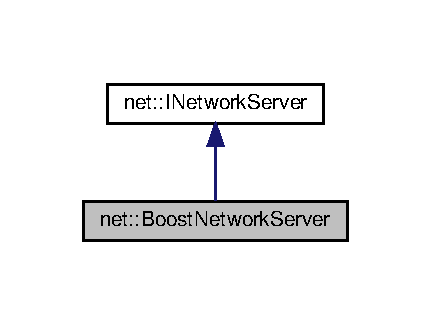
\includegraphics[width=207pt]{classnet_1_1BoostNetworkServer__inherit__graph}
\end{center}
\end{figure}


Collaboration diagram for net\+:\+:Boost\+Network\+Server\+:
\nopagebreak
\begin{figure}[H]
\begin{center}
\leavevmode
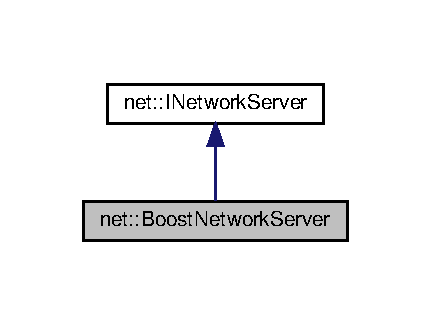
\includegraphics[width=207pt]{classnet_1_1BoostNetworkServer__coll__graph}
\end{center}
\end{figure}
\subsection*{Public Member Functions}
\begin{DoxyCompactItemize}
\item 
\mbox{\Hypertarget{classnet_1_1BoostNetworkServer_a0ab652342b8000e5192c67ab595fdc0b}\label{classnet_1_1BoostNetworkServer_a0ab652342b8000e5192c67ab595fdc0b}} 
{\bfseries Boost\+Network\+Server} (unsigned short port, const \hyperlink{classcore_1_1config_1_1Host}{core\+::config\+::\+Host} \&configs)
\item 
\mbox{\Hypertarget{classnet_1_1BoostNetworkServer_ad3ff8de9d2acf73bfbc264885bb1560d}\label{classnet_1_1BoostNetworkServer_ad3ff8de9d2acf73bfbc264885bb1560d}} 
void {\bfseries run} ()
\item 
\mbox{\Hypertarget{classnet_1_1BoostNetworkServer_a867c0aaca77e90d05ea7ba3136b4a7e3}\label{classnet_1_1BoostNetworkServer_a867c0aaca77e90d05ea7ba3136b4a7e3}} 
void {\bfseries stop} ()
\end{DoxyCompactItemize}


The documentation for this class was generated from the following files\+:\begin{DoxyCompactItemize}
\item 
inc/\+Network/\hyperlink{BoostNetworkServer_8hpp}{Boost\+Network\+Server.\+hpp}\item 
src/\+Network/Boost\+Network\+Server.\+cpp\end{DoxyCompactItemize}

\hypertarget{classihm_1_1CmdLine}{}\section{ihm\+:\+:Cmd\+Line Class Reference}
\label{classihm_1_1CmdLine}\index{ihm\+::\+Cmd\+Line@{ihm\+::\+Cmd\+Line}}


Interact with the user by tokenized string.  




{\ttfamily \#include $<$Cmd\+Line.\+hpp$>$}

\subsection*{Public Member Functions}
\begin{DoxyCompactItemize}
\item 
\mbox{\Hypertarget{classihm_1_1CmdLine_ad3bb0bb95b1e283b1fcd3e064f2ff393}\label{classihm_1_1CmdLine_ad3bb0bb95b1e283b1fcd3e064f2ff393}} 
\hyperlink{classihm_1_1CmdLine_ad3bb0bb95b1e283b1fcd3e064f2ff393}{Cmd\+Line} (\hyperlink{classcore_1_1ListenersControl}{core\+::\+Listeners\+Control} \&control)
\begin{DoxyCompactList}\small\item\em Construct a new Cmd Line object. \end{DoxyCompactList}\item 
\mbox{\Hypertarget{classihm_1_1CmdLine_a1fe3dd7c91f9662c9c84e8d8ebaf8423}\label{classihm_1_1CmdLine_a1fe3dd7c91f9662c9c84e8d8ebaf8423}} 
\hyperlink{classihm_1_1CmdLine_a1fe3dd7c91f9662c9c84e8d8ebaf8423}{$\sim$\+Cmd\+Line} ()
\begin{DoxyCompactList}\small\item\em Destroy the Cmd Line object. \end{DoxyCompactList}\item 
\mbox{\Hypertarget{classihm_1_1CmdLine_a35dec9782c4ff1e0bc5863dd919e1a10}\label{classihm_1_1CmdLine_a35dec9782c4ff1e0bc5863dd919e1a10}} 
\hyperlink{classcore_1_1ListenersControl}{core\+::\+Listeners\+Control} \& \hyperlink{classihm_1_1CmdLine_a35dec9782c4ff1e0bc5863dd919e1a10}{get\+Controller} () const
\begin{DoxyCompactList}\small\item\em Get the Controller object. \end{DoxyCompactList}\item 
\mbox{\Hypertarget{classihm_1_1CmdLine_abc24ef8ae2fcda3500f4d414051719a9}\label{classihm_1_1CmdLine_abc24ef8ae2fcda3500f4d414051719a9}} 
const std\+::vector$<$ \hyperlink{structihm_1_1command__t}{ihm\+::command\+\_\+t} $>$ \& \hyperlink{classihm_1_1CmdLine_abc24ef8ae2fcda3500f4d414051719a9}{get\+Commands\+Object} () const
\begin{DoxyCompactList}\small\item\em Return the commands object. \end{DoxyCompactList}\end{DoxyCompactItemize}


\subsection{Detailed Description}
Interact with the user by tokenized string. 

The documentation for this class was generated from the following files\+:\begin{DoxyCompactItemize}
\item 
inc/\+Ihm/\hyperlink{CmdLine_8hpp}{Cmd\+Line.\+hpp}\item 
src/\+Ihm/\hyperlink{CmdLine_8cpp}{Cmd\+Line.\+cpp}\end{DoxyCompactItemize}

\hypertarget{structihm_1_1command__t}{}\section{ihm\+:\+:command\+\_\+t Struct Reference}
\label{structihm_1_1command__t}\index{ihm\+::command\+\_\+t@{ihm\+::command\+\_\+t}}
\subsection*{Public Attributes}
\begin{DoxyCompactItemize}
\item 
\mbox{\Hypertarget{structihm_1_1command__t_a75af4a126696cfe61d9a615f8c20ec1a}\label{structihm_1_1command__t_a75af4a126696cfe61d9a615f8c20ec1a}} 
const std\+::string {\bfseries name}
\item 
\mbox{\Hypertarget{structihm_1_1command__t_ab6f55432fe6a0c9ad3135b44d8fb0202}\label{structihm_1_1command__t_ab6f55432fe6a0c9ad3135b44d8fb0202}} 
std\+::size\+\_\+t {\bfseries nb\+Params}
\item 
\mbox{\Hypertarget{structihm_1_1command__t_aa55ed142ffecd3c49fc1f20fa88b74fc}\label{structihm_1_1command__t_aa55ed142ffecd3c49fc1f20fa88b74fc}} 
void($\ast$ {\bfseries function} )(\hyperlink{classihm_1_1CmdLine}{ihm\+::\+Cmd\+Line} $\ast$, const std\+::vector$<$ std\+::string $>$ \&)
\item 
\mbox{\Hypertarget{structihm_1_1command__t_aebbf502a321be7cf5d0f4fbf8caa2148}\label{structihm_1_1command__t_aebbf502a321be7cf5d0f4fbf8caa2148}} 
const std\+::string {\bfseries description}
\end{DoxyCompactItemize}


The documentation for this struct was generated from the following file\+:\begin{DoxyCompactItemize}
\item 
inc/\+Ihm/\hyperlink{CmdLine_8hpp}{Cmd\+Line.\+hpp}\end{DoxyCompactItemize}

\hypertarget{classyconf_1_1ConfigNode}{}\section{yconf\+:\+:Config\+Node Class Reference}
\label{classyconf_1_1ConfigNode}\index{yconf\+::\+Config\+Node@{yconf\+::\+Config\+Node}}


Inheritance diagram for yconf\+:\+:Config\+Node\+:
\nopagebreak
\begin{figure}[H]
\begin{center}
\leavevmode
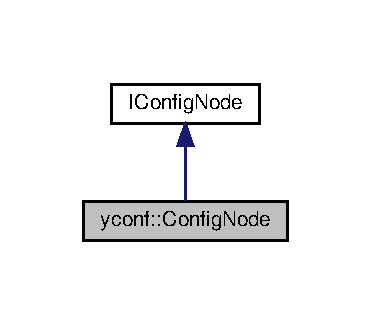
\includegraphics[width=178pt]{classyconf_1_1ConfigNode__inherit__graph}
\end{center}
\end{figure}


Collaboration diagram for yconf\+:\+:Config\+Node\+:
\nopagebreak
\begin{figure}[H]
\begin{center}
\leavevmode
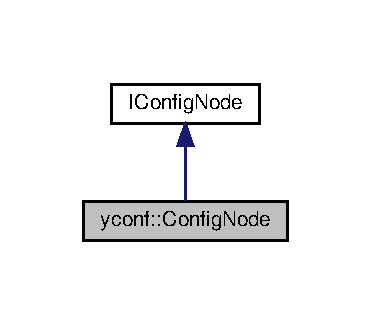
\includegraphics[width=178pt]{classyconf_1_1ConfigNode__coll__graph}
\end{center}
\end{figure}
\subsection*{Public Member Functions}
\begin{DoxyCompactItemize}
\item 
\mbox{\Hypertarget{classyconf_1_1ConfigNode_af12ecdf9ef85c2c121faf231e5c08429}\label{classyconf_1_1ConfigNode_af12ecdf9ef85c2c121faf231e5c08429}} 
\hyperlink{classyconf_1_1ConfigNode_af12ecdf9ef85c2c121faf231e5c08429}{Config\+Node} ()=default
\begin{DoxyCompactList}\small\item\em Config with no fields. \end{DoxyCompactList}\item 
\mbox{\Hypertarget{classyconf_1_1ConfigNode_a3f1d87cf39ea7f7e7b5588eca5ab3c2b}\label{classyconf_1_1ConfigNode_a3f1d87cf39ea7f7e7b5588eca5ab3c2b}} 
{\bfseries Config\+Node} (const std\+::string \&file\+Path)
\item 
\mbox{\Hypertarget{classyconf_1_1ConfigNode_a1d95531bcd3079100ab1fc75d97ff330}\label{classyconf_1_1ConfigNode_a1d95531bcd3079100ab1fc75d97ff330}} 
{\bfseries Config\+Node} (const Y\+A\+M\+L\+::\+Node \&root)
\item 
std\+::unique\+\_\+ptr$<$ \hyperlink{classIConfigNode}{I\+Config\+Node} $>$ \hyperlink{classyconf_1_1ConfigNode_a419f3e4e042f7cd0746f83d96977d18e}{get\+Child} (const std\+::string \&name) const override
\begin{DoxyCompactList}\small\item\em Gets a child node. \end{DoxyCompactList}\item 
std\+::string \hyperlink{classyconf_1_1ConfigNode_a4670a614581800cfaef06670ad2a0276}{get\+Value} (const std\+::string \&name) const override
\begin{DoxyCompactList}\small\item\em Gets the value of a property. \end{DoxyCompactList}\item 
std\+::vector$<$ std\+::string $>$ \hyperlink{classyconf_1_1ConfigNode_a4a1ed4e489687b3f1d4d514dbf57595d}{get\+Scalar\+Array} (const std\+::string \&name) const override
\begin{DoxyCompactList}\small\item\em Gets the content of the array, as scalars. \end{DoxyCompactList}\item 
std\+::vector$<$ std\+::unique\+\_\+ptr$<$ \hyperlink{classIConfigNode}{I\+Config\+Node} $>$ $>$ \hyperlink{classyconf_1_1ConfigNode_a3f590d4507699b6f9a9f3ca336f95255}{get\+Node\+Array} (const std\+::string \&name) const override
\begin{DoxyCompactList}\small\item\em Gets the content of the array, as nodes. \end{DoxyCompactList}\item 
std\+::unordered\+\_\+map$<$ std\+::string, std\+::string $>$ \hyperlink{classyconf_1_1ConfigNode_af15d6504faf3cf1be0aa5efc5603035f}{get\+All\+Scalars\+Of} (const std\+::string \&name) const override
\begin{DoxyCompactList}\small\item\em Returns all the properties from the node. \end{DoxyCompactList}\end{DoxyCompactItemize}


\subsection{Member Function Documentation}
\mbox{\Hypertarget{classyconf_1_1ConfigNode_af15d6504faf3cf1be0aa5efc5603035f}\label{classyconf_1_1ConfigNode_af15d6504faf3cf1be0aa5efc5603035f}} 
\index{yconf\+::\+Config\+Node@{yconf\+::\+Config\+Node}!get\+All\+Scalars\+Of@{get\+All\+Scalars\+Of}}
\index{get\+All\+Scalars\+Of@{get\+All\+Scalars\+Of}!yconf\+::\+Config\+Node@{yconf\+::\+Config\+Node}}
\subsubsection{\texorpdfstring{get\+All\+Scalars\+Of()}{getAllScalarsOf()}}
{\footnotesize\ttfamily std\+::unordered\+\_\+map$<$ std\+::string, std\+::string $>$ yconf\+::\+Config\+Node\+::get\+All\+Scalars\+Of (\begin{DoxyParamCaption}\item[{const std\+::string \&}]{name }\end{DoxyParamCaption}) const\hspace{0.3cm}{\ttfamily [override]}, {\ttfamily [virtual]}}



Returns all the properties from the node. 


\begin{DoxyParams}{Parameters}
{\em name} & The name of the wanted node If the name contains dot ({\ttfamily .}), it will get the child of the child, and so on until the last field that is the value name\\
\hline
\end{DoxyParams}
so {\ttfamily get\+All\+Scalars\+Of(\char`\"{}abc.\+def.\+xyz\char`\"{})} is the same as {\ttfamily get\+Child(\char`\"{}abc.\+def\char`\"{})-\/$>$get\+All\+Scalars\+Of(\char`\"{}xyz\char`\"{})}


\begin{DoxyExceptions}{Exceptions}
{\em $<$tt$>$std\+::out\+\_\+of\+\_\+range$<$/tt$>$} & if no such property exists \\
\hline
\end{DoxyExceptions}


Implements \hyperlink{classIConfigNode_ae6abd34301fc7141963ef125117db0c5}{I\+Config\+Node}.

\mbox{\Hypertarget{classyconf_1_1ConfigNode_a419f3e4e042f7cd0746f83d96977d18e}\label{classyconf_1_1ConfigNode_a419f3e4e042f7cd0746f83d96977d18e}} 
\index{yconf\+::\+Config\+Node@{yconf\+::\+Config\+Node}!get\+Child@{get\+Child}}
\index{get\+Child@{get\+Child}!yconf\+::\+Config\+Node@{yconf\+::\+Config\+Node}}
\subsubsection{\texorpdfstring{get\+Child()}{getChild()}}
{\footnotesize\ttfamily std\+::unique\+\_\+ptr$<$ \hyperlink{classIConfigNode}{I\+Config\+Node} $>$ yconf\+::\+Config\+Node\+::get\+Child (\begin{DoxyParamCaption}\item[{const std\+::string \&}]{name }\end{DoxyParamCaption}) const\hspace{0.3cm}{\ttfamily [override]}, {\ttfamily [virtual]}}



Gets a child node. 


\begin{DoxyParams}{Parameters}
{\em name} & Name of the wanted child node If the name contains dot ({\ttfamily .}), it will return the child of the child, and so on\\
\hline
\end{DoxyParams}
so {\ttfamily get\+Child(\char`\"{}abc.\+def.\+xyz\char`\"{})} is the same as {\ttfamily get\+Child(\char`\"{}abc\char`\"{})-\/$>$get\+Child(\char`\"{}def\char`\"{})-\/$>$get\+Child(\char`\"{}xyz\char`\"{})}

\begin{DoxyReturn}{Returns}
unique pointer to the child node 
\end{DoxyReturn}

\begin{DoxyExceptions}{Exceptions}
{\em $<$tt$>$std\+::out\+\_\+of\+\_\+range$<$/tt$>$} & if no such child exists \\
\hline
\end{DoxyExceptions}


Implements \hyperlink{classIConfigNode_a113e74aac6e8c62f5d5762b766f934e6}{I\+Config\+Node}.

\mbox{\Hypertarget{classyconf_1_1ConfigNode_a3f590d4507699b6f9a9f3ca336f95255}\label{classyconf_1_1ConfigNode_a3f590d4507699b6f9a9f3ca336f95255}} 
\index{yconf\+::\+Config\+Node@{yconf\+::\+Config\+Node}!get\+Node\+Array@{get\+Node\+Array}}
\index{get\+Node\+Array@{get\+Node\+Array}!yconf\+::\+Config\+Node@{yconf\+::\+Config\+Node}}
\subsubsection{\texorpdfstring{get\+Node\+Array()}{getNodeArray()}}
{\footnotesize\ttfamily std\+::vector$<$ std\+::unique\+\_\+ptr$<$ \hyperlink{classIConfigNode}{I\+Config\+Node} $>$ $>$ yconf\+::\+Config\+Node\+::get\+Node\+Array (\begin{DoxyParamCaption}\item[{const std\+::string \&}]{name }\end{DoxyParamCaption}) const\hspace{0.3cm}{\ttfamily [override]}, {\ttfamily [virtual]}}



Gets the content of the array, as nodes. 


\begin{DoxyParams}{Parameters}
{\em name} & The name of the wanted array If the name contains dot ({\ttfamily .}), it will get the child of the child, and so on until the last field that is the value name\\
\hline
\end{DoxyParams}
so {\ttfamily get\+Node\+Array(\char`\"{}abc.\+def.\+xyz\char`\"{})} is the same as {\ttfamily get\+Child(\char`\"{}abc.\+def\char`\"{})-\/$>$get\+Node\+Array(\char`\"{}xyz\char`\"{})}

\begin{DoxyReturn}{Returns}
Array content as nodes 
\end{DoxyReturn}

\begin{DoxyExceptions}{Exceptions}
{\em $<$tt$>$std\+::out\+\_\+of\+\_\+range$<$/tt$>$} & if no such property exists \\
\hline
\end{DoxyExceptions}


Implements \hyperlink{classIConfigNode_a3a15562e0598f5bb105ddd006e298157}{I\+Config\+Node}.

\mbox{\Hypertarget{classyconf_1_1ConfigNode_a4a1ed4e489687b3f1d4d514dbf57595d}\label{classyconf_1_1ConfigNode_a4a1ed4e489687b3f1d4d514dbf57595d}} 
\index{yconf\+::\+Config\+Node@{yconf\+::\+Config\+Node}!get\+Scalar\+Array@{get\+Scalar\+Array}}
\index{get\+Scalar\+Array@{get\+Scalar\+Array}!yconf\+::\+Config\+Node@{yconf\+::\+Config\+Node}}
\subsubsection{\texorpdfstring{get\+Scalar\+Array()}{getScalarArray()}}
{\footnotesize\ttfamily std\+::vector$<$ std\+::string $>$ yconf\+::\+Config\+Node\+::get\+Scalar\+Array (\begin{DoxyParamCaption}\item[{const std\+::string \&}]{name }\end{DoxyParamCaption}) const\hspace{0.3cm}{\ttfamily [override]}, {\ttfamily [virtual]}}



Gets the content of the array, as scalars. 


\begin{DoxyParams}{Parameters}
{\em name} & The name of the wanted array If the name contains dot ({\ttfamily .}), it will get the child of the child, and so on until the last field that is the value name\\
\hline
\end{DoxyParams}
so {\ttfamily get\+Scalar\+Array(\char`\"{}abc.\+def.\+xyz\char`\"{})} is the same as {\ttfamily get\+Child(\char`\"{}abc.\+def\char`\"{})-\/$>$get\+Scalar\+Array(\char`\"{}xyz\char`\"{})}

\begin{DoxyReturn}{Returns}
Array content as scalar 
\end{DoxyReturn}

\begin{DoxyExceptions}{Exceptions}
{\em $<$tt$>$std\+::out\+\_\+of\+\_\+range$<$/tt$>$} & if no such property exists \\
\hline
\end{DoxyExceptions}


Implements \hyperlink{classIConfigNode_aaa66c9d23d521b5b5c9f5f6bf35087fb}{I\+Config\+Node}.

\mbox{\Hypertarget{classyconf_1_1ConfigNode_a4670a614581800cfaef06670ad2a0276}\label{classyconf_1_1ConfigNode_a4670a614581800cfaef06670ad2a0276}} 
\index{yconf\+::\+Config\+Node@{yconf\+::\+Config\+Node}!get\+Value@{get\+Value}}
\index{get\+Value@{get\+Value}!yconf\+::\+Config\+Node@{yconf\+::\+Config\+Node}}
\subsubsection{\texorpdfstring{get\+Value()}{getValue()}}
{\footnotesize\ttfamily std\+::string yconf\+::\+Config\+Node\+::get\+Value (\begin{DoxyParamCaption}\item[{const std\+::string \&}]{name }\end{DoxyParamCaption}) const\hspace{0.3cm}{\ttfamily [override]}, {\ttfamily [virtual]}}



Gets the value of a property. 


\begin{DoxyParams}{Parameters}
{\em name} & The name of the wanted property If the name contains dot ({\ttfamily .}), it will get the child of the child, and so on until the last field that is the value name\\
\hline
\end{DoxyParams}
so {\ttfamily get\+Value(\char`\"{}abc.\+def.\+xyz\char`\"{})} is the same as {\ttfamily get\+Child(\char`\"{}abc.\+def\char`\"{})-\/$>$get\+Value(\char`\"{}xyz\char`\"{})}

\begin{DoxyReturn}{Returns}
Property value 
\end{DoxyReturn}

\begin{DoxyExceptions}{Exceptions}
{\em $<$tt$>$std\+::out\+\_\+of\+\_\+range$<$/tt$>$} & if no such property exists \\
\hline
\end{DoxyExceptions}


Implements \hyperlink{classIConfigNode_ae32a49d812d3f98cbc048ab3cce5f7d6}{I\+Config\+Node}.



The documentation for this class was generated from the following files\+:\begin{DoxyCompactItemize}
\item 
inc/yconf/Config\+Node.\+hpp\item 
src/Config\+Node.\+cpp\end{DoxyCompactItemize}

\hypertarget{classcore_1_1Configurations}{}\section{core\+:\+:Configurations Class Reference}
\label{classcore_1_1Configurations}\index{core\+::\+Configurations@{core\+::\+Configurations}}
\subsection*{Public Member Functions}
\begin{DoxyCompactItemize}
\item 
\mbox{\Hypertarget{classcore_1_1Configurations_a162460996859d9182b1dd9b146d22639}\label{classcore_1_1Configurations_a162460996859d9182b1dd9b146d22639}} 
{\bfseries Configurations} (const std\+::string \&filename)
\item 
\mbox{\Hypertarget{classcore_1_1Configurations_a6b1904b8f7e31a707dff507d610776f8}\label{classcore_1_1Configurations_a6b1904b8f7e31a707dff507d610776f8}} 
void {\bfseries update\+Path} (const std\+::string \&filename)
\item 
\mbox{\Hypertarget{classcore_1_1Configurations_a99bb4c3ad7d0a1d0bd88469937a11df7}\label{classcore_1_1Configurations_a99bb4c3ad7d0a1d0bd88469937a11df7}} 
void {\bfseries reload} ()
\item 
\mbox{\Hypertarget{classcore_1_1Configurations_abc8a042d0f01de39311c8b12f3bb7caa}\label{classcore_1_1Configurations_abc8a042d0f01de39311c8b12f3bb7caa}} 
void {\bfseries print} () const
\item 
\mbox{\Hypertarget{classcore_1_1Configurations_a2a2ef7171b6c8b98f8adb4f0a63a5bf8}\label{classcore_1_1Configurations_a2a2ef7171b6c8b98f8adb4f0a63a5bf8}} 
const \hyperlink{classcore_1_1config_1_1Host}{core\+::config\+::\+Host} \& {\bfseries get\+Host\+By\+Domain} (const std\+::string \&domain) const
\item 
\mbox{\Hypertarget{classcore_1_1Configurations_a651e5195e625473c4994f9e7e7b4fa14}\label{classcore_1_1Configurations_a651e5195e625473c4994f9e7e7b4fa14}} 
const \hyperlink{classcore_1_1config_1_1Host}{core\+::config\+::\+Host} \& {\bfseries get\+Host\+By\+Port} (unsigned short port) const
\item 
\mbox{\Hypertarget{classcore_1_1Configurations_ad95b237ce411d5a442647ff53b9e80f1}\label{classcore_1_1Configurations_ad95b237ce411d5a442647ff53b9e80f1}} 
const std\+::vector$<$ \hyperlink{classcore_1_1config_1_1Host}{core\+::config\+::\+Host} $>$ \& {\bfseries get\+Hosts} () const
\end{DoxyCompactItemize}
\subsection*{Static Public Member Functions}
\begin{DoxyCompactItemize}
\item 
\mbox{\Hypertarget{classcore_1_1Configurations_a90f881cfb6b5b430afb3abcb77de5b06}\label{classcore_1_1Configurations_a90f881cfb6b5b430afb3abcb77de5b06}} 
static std\+::vector$<$ std\+::string $>$ {\bfseries get\+All\+Dyn\+Name} ()
\end{DoxyCompactItemize}
\subsection*{Static Public Attributes}
\begin{DoxyCompactItemize}
\item 
\mbox{\Hypertarget{classcore_1_1Configurations_a36fd6acfda020ebe632b4bf285dbc24b}\label{classcore_1_1Configurations_a36fd6acfda020ebe632b4bf285dbc24b}} 
static std\+::string {\bfseries modules\+Path}
\end{DoxyCompactItemize}


The documentation for this class was generated from the following files\+:\begin{DoxyCompactItemize}
\item 
inc/\+Core/\+Configs/\hyperlink{Configurations_8hpp}{Configurations.\+hpp}\item 
src/\+Core/\+Configs/\hyperlink{Configurations_8cpp}{Configurations.\+cpp}\end{DoxyCompactItemize}

\hypertarget{classFakeClient}{}\section{Fake\+Client Class Reference}
\label{classFakeClient}\index{Fake\+Client@{Fake\+Client}}


Inheritance diagram for Fake\+Client\+:
\nopagebreak
\begin{figure}[H]
\begin{center}
\leavevmode
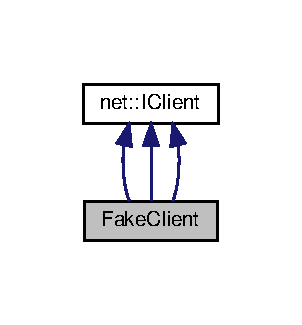
\includegraphics[width=145pt]{classFakeClient__inherit__graph}
\end{center}
\end{figure}


Collaboration diagram for Fake\+Client\+:
\nopagebreak
\begin{figure}[H]
\begin{center}
\leavevmode
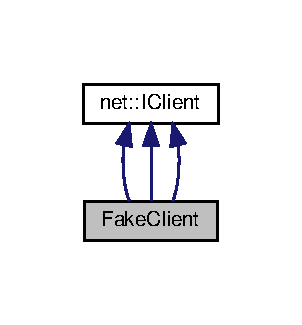
\includegraphics[width=145pt]{classFakeClient__coll__graph}
\end{center}
\end{figure}
\subsection*{Additional Inherited Members}


The documentation for this class was generated from the following files\+:\begin{DoxyCompactItemize}
\item 
tests/\hyperlink{ModuleFile_8cpp}{Module\+File.\+cpp}\item 
tests/\hyperlink{ModulePhp_8cpp}{Module\+Php.\+cpp}\item 
tests/\hyperlink{ModuleProxy_8cpp}{Module\+Proxy.\+cpp}\end{DoxyCompactItemize}

\hypertarget{classmodule_1_1File}{}\section{module\+:\+:File Class Reference}
\label{classmodule_1_1File}\index{module\+::\+File@{module\+::\+File}}


Inheritance diagram for module\+:\+:File\+:
\nopagebreak
\begin{figure}[H]
\begin{center}
\leavevmode
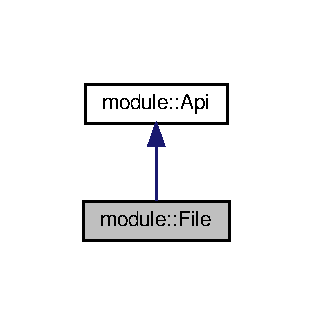
\includegraphics[width=150pt]{classmodule_1_1File__inherit__graph}
\end{center}
\end{figure}


Collaboration diagram for module\+:\+:File\+:
\nopagebreak
\begin{figure}[H]
\begin{center}
\leavevmode
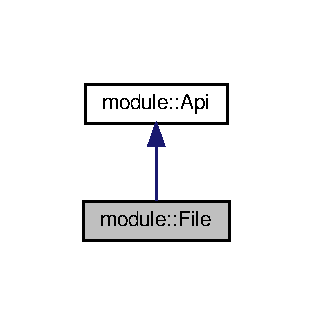
\includegraphics[width=150pt]{classmodule_1_1File__coll__graph}
\end{center}
\end{figure}
\subsection*{Public Member Functions}
\begin{DoxyCompactItemize}
\item 
\mbox{\Hypertarget{classmodule_1_1File_ada1db6c6a7d23d119c470a0da3249753}\label{classmodule_1_1File_ada1db6c6a7d23d119c470a0da3249753}} 
std\+::string \hyperlink{classmodule_1_1File_ada1db6c6a7d23d119c470a0da3249753}{name} () const noexcept
\begin{DoxyCompactList}\small\item\em Returns the module name. \end{DoxyCompactList}\item 
bool \hyperlink{classmodule_1_1File_a369f5f98cfbc477e345b7372319737d7}{new\+Connection} (const \hyperlink{structnet_1_1IClient}{net\+::\+I\+Client} \&client) noexcept
\begin{DoxyCompactList}\small\item\em When a new client connects to the http server. \end{DoxyCompactList}\item 
bool \hyperlink{classmodule_1_1File_a86bd2e04ae5946fb790342911b9e4454}{disconnection} (const \hyperlink{structnet_1_1IClient}{net\+::\+I\+Client} \&client) noexcept
\begin{DoxyCompactList}\small\item\em When a client disconnects. \end{DoxyCompactList}\item 
\mbox{\Hypertarget{classmodule_1_1File_a017d7a3238a03237d62739c67de5b2b8}\label{classmodule_1_1File_a017d7a3238a03237d62739c67de5b2b8}} 
bool \hyperlink{classmodule_1_1File_a017d7a3238a03237d62739c67de5b2b8}{set\+Configurations} (Configs configs) noexcept
\begin{DoxyCompactList}\small\item\em Set the Global configs of the module. \end{DoxyCompactList}\item 
bool \hyperlink{classmodule_1_1File_af37dc06c40ef291f3789ae4b00e628d7}{after\+Receive} (const \hyperlink{structnet_1_1IClient}{net\+::\+I\+Client} \&client, std\+::string \&buffer) noexcept
\begin{DoxyCompactList}\small\item\em Just before the deserialization of the packet. \end{DoxyCompactList}\item 
bool \hyperlink{classmodule_1_1File_a201c3c9c01df460e22f270c554937639}{after\+Unpacked} (const \hyperlink{structnet_1_1IClient}{net\+::\+I\+Client} \&client, \hyperlink{structhttp_1_1IRequest}{http\+::\+I\+Request} \&request) noexcept
\begin{DoxyCompactList}\small\item\em Call before the main behavior of the module. \end{DoxyCompactList}\item 
bool \hyperlink{classmodule_1_1File_a7fceec434dd7b735e08b01a5bd16625b}{execute} (const \hyperlink{structnet_1_1IClient}{net\+::\+I\+Client} \&client, \hyperlink{structhttp_1_1IRequest}{http\+::\+I\+Request} \&request, \hyperlink{structhttp_1_1IResponse}{http\+::\+I\+Response} \&response) noexcept
\begin{DoxyCompactList}\small\item\em This is the main behavior of the module. \end{DoxyCompactList}\item 
bool \hyperlink{classmodule_1_1File_ab2004b38d5dd63e0e19f358a3820477f}{before\+Packed} (const \hyperlink{structnet_1_1IClient}{net\+::\+I\+Client} \&client, \hyperlink{structhttp_1_1IResponse}{http\+::\+I\+Response} \&response) noexcept
\begin{DoxyCompactList}\small\item\em Just before the serialization of the response. \end{DoxyCompactList}\item 
bool \hyperlink{classmodule_1_1File_a13091749fbe954576d351e90e15581d7}{before\+Send} (const \hyperlink{structnet_1_1IClient}{net\+::\+I\+Client} \&client, std\+::string \&buffer) noexcept
\begin{DoxyCompactList}\small\item\em Just before packet delivery. \end{DoxyCompactList}\end{DoxyCompactItemize}


\subsection{Member Function Documentation}
\mbox{\Hypertarget{classmodule_1_1File_af37dc06c40ef291f3789ae4b00e628d7}\label{classmodule_1_1File_af37dc06c40ef291f3789ae4b00e628d7}} 
\index{module\+::\+File@{module\+::\+File}!after\+Receive@{after\+Receive}}
\index{after\+Receive@{after\+Receive}!module\+::\+File@{module\+::\+File}}
\subsubsection{\texorpdfstring{after\+Receive()}{afterReceive()}}
{\footnotesize\ttfamily bool module\+::\+File\+::after\+Receive (\begin{DoxyParamCaption}\item[{const \hyperlink{structnet_1_1IClient}{net\+::\+I\+Client} \&}]{client,  }\item[{std\+::string \&}]{buffer }\end{DoxyParamCaption})\hspace{0.3cm}{\ttfamily [virtual]}, {\ttfamily [noexcept]}}



Just before the deserialization of the packet. 

It can be useful to decrypt an tls packet 

Implements \hyperlink{structmodule_1_1Api_ad8b56820e4f53bf65d34447184edef20}{module\+::\+Api}.

\mbox{\Hypertarget{classmodule_1_1File_a201c3c9c01df460e22f270c554937639}\label{classmodule_1_1File_a201c3c9c01df460e22f270c554937639}} 
\index{module\+::\+File@{module\+::\+File}!after\+Unpacked@{after\+Unpacked}}
\index{after\+Unpacked@{after\+Unpacked}!module\+::\+File@{module\+::\+File}}
\subsubsection{\texorpdfstring{after\+Unpacked()}{afterUnpacked()}}
{\footnotesize\ttfamily bool module\+::\+File\+::after\+Unpacked (\begin{DoxyParamCaption}\item[{const \hyperlink{structnet_1_1IClient}{net\+::\+I\+Client} \&}]{client,  }\item[{\hyperlink{structhttp_1_1IRequest}{http\+::\+I\+Request} \&}]{request }\end{DoxyParamCaption})\hspace{0.3cm}{\ttfamily [virtual]}, {\ttfamily [noexcept]}}



Call before the main behavior of the module. 

It can be useful to decompresses a http body (gzip, ...) 

Implements \hyperlink{structmodule_1_1Api_a291297e6d233e69b82c976e085f7c237}{module\+::\+Api}.

\mbox{\Hypertarget{classmodule_1_1File_ab2004b38d5dd63e0e19f358a3820477f}\label{classmodule_1_1File_ab2004b38d5dd63e0e19f358a3820477f}} 
\index{module\+::\+File@{module\+::\+File}!before\+Packed@{before\+Packed}}
\index{before\+Packed@{before\+Packed}!module\+::\+File@{module\+::\+File}}
\subsubsection{\texorpdfstring{before\+Packed()}{beforePacked()}}
{\footnotesize\ttfamily bool module\+::\+File\+::before\+Packed (\begin{DoxyParamCaption}\item[{const \hyperlink{structnet_1_1IClient}{net\+::\+I\+Client} \&}]{client,  }\item[{\hyperlink{structhttp_1_1IResponse}{http\+::\+I\+Response} \&}]{response }\end{DoxyParamCaption})\hspace{0.3cm}{\ttfamily [virtual]}, {\ttfamily [noexcept]}}



Just before the serialization of the response. 

Useful if we need to add something in the packet or to compress it 

Implements \hyperlink{structmodule_1_1Api_a5293babe6b28a397b7a11f32da0a6f51}{module\+::\+Api}.

\mbox{\Hypertarget{classmodule_1_1File_a13091749fbe954576d351e90e15581d7}\label{classmodule_1_1File_a13091749fbe954576d351e90e15581d7}} 
\index{module\+::\+File@{module\+::\+File}!before\+Send@{before\+Send}}
\index{before\+Send@{before\+Send}!module\+::\+File@{module\+::\+File}}
\subsubsection{\texorpdfstring{before\+Send()}{beforeSend()}}
{\footnotesize\ttfamily bool module\+::\+File\+::before\+Send (\begin{DoxyParamCaption}\item[{const \hyperlink{structnet_1_1IClient}{net\+::\+I\+Client} \&}]{client,  }\item[{std\+::string \&}]{buffer }\end{DoxyParamCaption})\hspace{0.3cm}{\ttfamily [virtual]}, {\ttfamily [noexcept]}}



Just before packet delivery. 

Useful if we need to add something in the packet or to encrypt 

Implements \hyperlink{structmodule_1_1Api_a71d1ada8bc5fc81fd71607315dd86185}{module\+::\+Api}.

\mbox{\Hypertarget{classmodule_1_1File_a86bd2e04ae5946fb790342911b9e4454}\label{classmodule_1_1File_a86bd2e04ae5946fb790342911b9e4454}} 
\index{module\+::\+File@{module\+::\+File}!disconnection@{disconnection}}
\index{disconnection@{disconnection}!module\+::\+File@{module\+::\+File}}
\subsubsection{\texorpdfstring{disconnection()}{disconnection()}}
{\footnotesize\ttfamily bool module\+::\+File\+::disconnection (\begin{DoxyParamCaption}\item[{const \hyperlink{structnet_1_1IClient}{net\+::\+I\+Client} \&}]{client }\end{DoxyParamCaption})\hspace{0.3cm}{\ttfamily [virtual]}, {\ttfamily [noexcept]}}



When a client disconnects. 

To inform the module of the client\textquotesingle{}s disconnection 

Implements \hyperlink{structmodule_1_1Api_a8aa98bd4094fb13916e100509a948763}{module\+::\+Api}.

\mbox{\Hypertarget{classmodule_1_1File_a7fceec434dd7b735e08b01a5bd16625b}\label{classmodule_1_1File_a7fceec434dd7b735e08b01a5bd16625b}} 
\index{module\+::\+File@{module\+::\+File}!execute@{execute}}
\index{execute@{execute}!module\+::\+File@{module\+::\+File}}
\subsubsection{\texorpdfstring{execute()}{execute()}}
{\footnotesize\ttfamily bool module\+::\+File\+::execute (\begin{DoxyParamCaption}\item[{const \hyperlink{structnet_1_1IClient}{net\+::\+I\+Client} \&}]{client,  }\item[{\hyperlink{structhttp_1_1IRequest}{http\+::\+I\+Request} \&}]{request,  }\item[{\hyperlink{structhttp_1_1IResponse}{http\+::\+I\+Response} \&}]{response }\end{DoxyParamCaption})\hspace{0.3cm}{\ttfamily [virtual]}, {\ttfamily [noexcept]}}



This is the main behavior of the module. 

Reaction to the client\textquotesingle{}s request 

Implements \hyperlink{structmodule_1_1Api_afd1f5243a90811d06d96f725490bcba6}{module\+::\+Api}.

\mbox{\Hypertarget{classmodule_1_1File_a369f5f98cfbc477e345b7372319737d7}\label{classmodule_1_1File_a369f5f98cfbc477e345b7372319737d7}} 
\index{module\+::\+File@{module\+::\+File}!new\+Connection@{new\+Connection}}
\index{new\+Connection@{new\+Connection}!module\+::\+File@{module\+::\+File}}
\subsubsection{\texorpdfstring{new\+Connection()}{newConnection()}}
{\footnotesize\ttfamily bool module\+::\+File\+::new\+Connection (\begin{DoxyParamCaption}\item[{const \hyperlink{structnet_1_1IClient}{net\+::\+I\+Client} \&}]{client }\end{DoxyParamCaption})\hspace{0.3cm}{\ttfamily [virtual]}, {\ttfamily [noexcept]}}



When a new client connects to the http server. 

It can be useful to store the id of the client to recognize him after 

Implements \hyperlink{structmodule_1_1Api_aa83ddc92765200dd65f915498175c2be}{module\+::\+Api}.



The documentation for this class was generated from the following files\+:\begin{DoxyCompactItemize}
\item 
modules/\+File/\hyperlink{File_8hpp}{File.\+hpp}\item 
modules/\+File/\hyperlink{File_8cpp}{File.\+cpp}\end{DoxyCompactItemize}

\hypertarget{classcore_1_1config_1_1Host}{}\section{core\+:\+:config\+:\+:Host Class Reference}
\label{classcore_1_1config_1_1Host}\index{core\+::config\+::\+Host@{core\+::config\+::\+Host}}


Inheritance diagram for core\+:\+:config\+:\+:Host\+:
\nopagebreak
\begin{figure}[H]
\begin{center}
\leavevmode
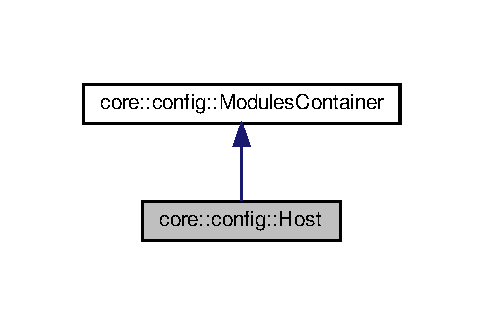
\includegraphics[width=232pt]{classcore_1_1config_1_1Host__inherit__graph}
\end{center}
\end{figure}


Collaboration diagram for core\+:\+:config\+:\+:Host\+:
\nopagebreak
\begin{figure}[H]
\begin{center}
\leavevmode
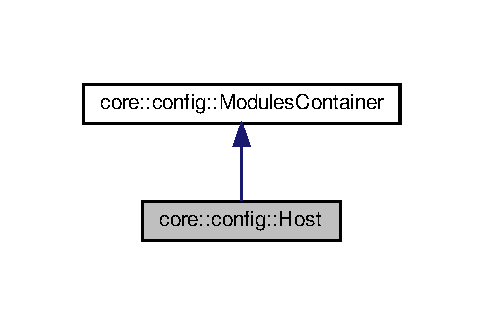
\includegraphics[width=232pt]{classcore_1_1config_1_1Host__coll__graph}
\end{center}
\end{figure}
\subsection*{Public Member Functions}
\begin{DoxyCompactItemize}
\item 
\mbox{\Hypertarget{classcore_1_1config_1_1Host_ab5608aa941f9801c303be4a4f6a92bd9}\label{classcore_1_1config_1_1Host_ab5608aa941f9801c303be4a4f6a92bd9}} 
{\bfseries Host} (const \hyperlink{classIConfigNode}{I\+Config\+Node} \&node)
\item 
\mbox{\Hypertarget{classcore_1_1config_1_1Host_a1ce4d7d648965b68baaec038d729659c}\label{classcore_1_1config_1_1Host_a1ce4d7d648965b68baaec038d729659c}} 
std\+::string {\bfseries get\+Domain} () const
\item 
\mbox{\Hypertarget{classcore_1_1config_1_1Host_a3de75f501fae836e3640880b3edc5ee2}\label{classcore_1_1config_1_1Host_a3de75f501fae836e3640880b3edc5ee2}} 
std\+::uint16\+\_\+t {\bfseries get\+Port} () const
\item 
\mbox{\Hypertarget{classcore_1_1config_1_1Host_afcfb19681ef50cb4f2fe2a94ae52976a}\label{classcore_1_1config_1_1Host_afcfb19681ef50cb4f2fe2a94ae52976a}} 
bool {\bfseries is\+Route\+Match} (const std\+::string uri) const
\item 
\mbox{\Hypertarget{classcore_1_1config_1_1Host_ab7c1b67a94d1c6a760a7b22b32824a40}\label{classcore_1_1config_1_1Host_ab7c1b67a94d1c6a760a7b22b32824a40}} 
const \hyperlink{classcore_1_1config_1_1Route}{core\+::config\+::\+Route} \& {\bfseries get\+Route\+By\+Match} (const std\+::string \&uri) const
\item 
\mbox{\Hypertarget{classcore_1_1config_1_1Host_a78f5c42a8c63d04a96fafba8cf073e92}\label{classcore_1_1config_1_1Host_a78f5c42a8c63d04a96fafba8cf073e92}} 
const \hyperlink{classcore_1_1config_1_1Route}{core\+::config\+::\+Route} \& {\bfseries get\+Route\+By\+Name} (const std\+::string \&name) const
\item 
\mbox{\Hypertarget{classcore_1_1config_1_1Host_ae76f1a298a1266206bb4727ad95ca549}\label{classcore_1_1config_1_1Host_ae76f1a298a1266206bb4727ad95ca549}} 
const std\+::vector$<$ \hyperlink{classcore_1_1config_1_1Route}{core\+::config\+::\+Route} $>$ \& {\bfseries get\+Routes} () const
\end{DoxyCompactItemize}
\subsection*{Additional Inherited Members}


The documentation for this class was generated from the following files\+:\begin{DoxyCompactItemize}
\item 
inc/\+Core/\+Configs/\hyperlink{Host_8hpp}{Host.\+hpp}\item 
src/\+Core/\+Configs/\hyperlink{Host_8cpp}{Host.\+cpp}\end{DoxyCompactItemize}

\hypertarget{classHttpRequest}{}\section{Http\+Request Class Reference}
\label{classHttpRequest}\index{Http\+Request@{Http\+Request}}


Inheritance diagram for Http\+Request\+:
\nopagebreak
\begin{figure}[H]
\begin{center}
\leavevmode
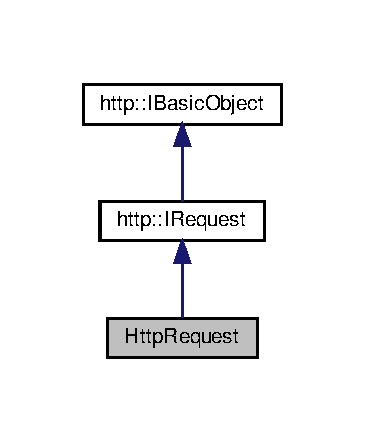
\includegraphics[width=175pt]{classHttpRequest__inherit__graph}
\end{center}
\end{figure}


Collaboration diagram for Http\+Request\+:
\nopagebreak
\begin{figure}[H]
\begin{center}
\leavevmode
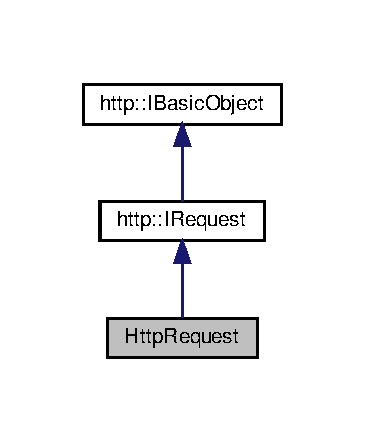
\includegraphics[width=175pt]{classHttpRequest__coll__graph}
\end{center}
\end{figure}
\subsection*{Public Member Functions}
\begin{DoxyCompactItemize}
\item 
\mbox{\Hypertarget{classHttpRequest_a5b93c0ff7316f034cb556da01dd4e44c}\label{classHttpRequest_a5b93c0ff7316f034cb556da01dd4e44c}} 
{\bfseries Http\+Request} (std\+::string request)
\item 
http\+::\+Verb \hyperlink{classHttpRequest_aded380ba96f29fb1cc6da1679a975dd8}{verb} () const noexcept
\begin{DoxyCompactList}\small\item\em Returns the http verb. \end{DoxyCompactList}\item 
bool \hyperlink{classHttpRequest_a243897d5dd8ba0195ce0acb6e9dd79ae}{verb} (http\+::\+Verb verb) noexcept
\begin{DoxyCompactList}\small\item\em Change the verb of the request. \end{DoxyCompactList}\item 
std\+::string \hyperlink{classHttpRequest_a313930a1717c2635ad092b7f6c7d2460}{route} () const noexcept
\begin{DoxyCompactList}\small\item\em Returns the route. \end{DoxyCompactList}\item 
bool \hyperlink{classHttpRequest_aa71843738db71fe1f826bd30fbf5bb29}{route} (std\+::string route) noexcept
\begin{DoxyCompactList}\small\item\em Change the route. \end{DoxyCompactList}\item 
bool \hyperlink{classHttpRequest_a81ce6a379efeba53bd3d40699462628b}{query\+Parameter\+Exist} (const std\+::string \&key) const noexcept
\begin{DoxyCompactList}\small\item\em Checks if in the route, there are a named \textquotesingle{}key\textquotesingle{} query parameter. \end{DoxyCompactList}\item 
std\+::string \hyperlink{classHttpRequest_a10cef7d5ff51ddc7eb5ebd2f25a0f66c}{query\+Parameter} (const std\+::string \&key) const noexcept
\begin{DoxyCompactList}\small\item\em Return the query parameter \char`\"{}key\char`\"{} found in the route. \end{DoxyCompactList}\item 
bool \hyperlink{classHttpRequest_a09bf36e9a2c76927ee45e6c5c699c461}{query\+Parameter} (std\+::string key, std\+::string value) noexcept
\begin{DoxyCompactList}\small\item\em Add / Update a query parameter. \end{DoxyCompactList}\item 
\mbox{\Hypertarget{classHttpRequest_abc502aa6bf23ed6cdecfa25f36dc3eb9}\label{classHttpRequest_abc502aa6bf23ed6cdecfa25f36dc3eb9}} 
std\+::string \hyperlink{classHttpRequest_abc502aa6bf23ed6cdecfa25f36dc3eb9}{cookie} (const std\+::string \&name) const noexcept
\begin{DoxyCompactList}\small\item\em Return the value of the cookie \textquotesingle{}name\textquotesingle{} In header there are an header parameter name \textquotesingle{}Cookie\textquotesingle{} who has all cookies of the request ex\+: \char`\"{}\+Cookie\+: yummy\+\_\+cookie=choco; tasty\+\_\+cookie=strawberry\char`\"{} Return a empty string if the cookie not exist. \end{DoxyCompactList}\item 
\mbox{\Hypertarget{classHttpRequest_afa7c70d447bee6e233488d66e9cc1c21}\label{classHttpRequest_afa7c70d447bee6e233488d66e9cc1c21}} 
std\+::string \hyperlink{classHttpRequest_afa7c70d447bee6e233488d66e9cc1c21}{protocol} () const noexcept
\begin{DoxyCompactList}\small\item\em Return the protocol of the object. \end{DoxyCompactList}\item 
bool \hyperlink{classHttpRequest_a74ea75d8685647989346bd5d1d25702a}{header\+Parameter\+Exist} (const std\+::string \&key) const noexcept
\begin{DoxyCompactList}\small\item\em Checks if in object, there are a named \textquotesingle{}key\textquotesingle{} header parameter. \end{DoxyCompactList}\item 
std\+::string \hyperlink{classHttpRequest_a96f232879fff933182a3ed5c80229df6}{header\+Parameter} (const std\+::string \&key) const noexcept
\begin{DoxyCompactList}\small\item\em Return the header parameter \char`\"{}key\char`\"{} found in the object. \end{DoxyCompactList}\item 
bool \hyperlink{classHttpRequest_a04f974104da7c06c568a8e648693e92c}{header\+Parameter} (std\+::string key, std\+::string value) noexcept
\begin{DoxyCompactList}\small\item\em Add / Update a header parameter. \end{DoxyCompactList}\item 
std\+::string \hyperlink{classHttpRequest_a16be46a53c2d2f8d29ad89aa213f30bb}{body} () const noexcept
\begin{DoxyCompactList}\small\item\em Return the body of the object. \end{DoxyCompactList}\item 
bool \hyperlink{classHttpRequest_a591fb5ec9430764ed5b3578d49c3858f}{body} (std\+::string body) noexcept
\begin{DoxyCompactList}\small\item\em Set / Add a new body in the object. \end{DoxyCompactList}\item 
bool \hyperlink{classHttpRequest_afd8f9f22651d2844b7b2d4cb882b7e19}{body\+Append} (std\+::string \hyperlink{classHttpRequest_a16be46a53c2d2f8d29ad89aa213f30bb}{body}) noexcept
\begin{DoxyCompactList}\small\item\em Append data in the body or create it if not exist. \end{DoxyCompactList}\item 
\mbox{\Hypertarget{classHttpRequest_a3acde34debb29c7e14fc6fd85f9fb49c}\label{classHttpRequest_a3acde34debb29c7e14fc6fd85f9fb49c}} 
std\+::string \hyperlink{classHttpRequest_a3acde34debb29c7e14fc6fd85f9fb49c}{serialize} () const noexcept
\begin{DoxyCompactList}\small\item\em Transform this object in a true http object. \end{DoxyCompactList}\end{DoxyCompactItemize}
\subsection*{Public Attributes}
\begin{DoxyCompactItemize}
\item 
\mbox{\Hypertarget{classHttpRequest_a95233407ba39db8e17b3d330158ad734}\label{classHttpRequest_a95233407ba39db8e17b3d330158ad734}} 
std\+::unordered\+\_\+map$<$ std\+::string, http\+::\+Verb $>$ {\bfseries map\+\_\+request\+\_\+method}
\item 
\mbox{\Hypertarget{classHttpRequest_aefc311390bef414d9509b27a81dd9578}\label{classHttpRequest_aefc311390bef414d9509b27a81dd9578}} 
std\+::unordered\+\_\+map$<$ std\+::string, std\+::string $>$ {\bfseries url\+\_\+encode}
\end{DoxyCompactItemize}


\subsection{Member Function Documentation}
\mbox{\Hypertarget{classHttpRequest_a16be46a53c2d2f8d29ad89aa213f30bb}\label{classHttpRequest_a16be46a53c2d2f8d29ad89aa213f30bb}} 
\index{Http\+Request@{Http\+Request}!body@{body}}
\index{body@{body}!Http\+Request@{Http\+Request}}
\subsubsection{\texorpdfstring{body()}{body()}\hspace{0.1cm}{\footnotesize\ttfamily [1/2]}}
{\footnotesize\ttfamily std\+::string Http\+Request\+::body (\begin{DoxyParamCaption}{ }\end{DoxyParamCaption}) const\hspace{0.3cm}{\ttfamily [virtual]}, {\ttfamily [noexcept]}}



Return the body of the object. 

Sometimes in object like P\+O\+ST there are a body He can take any form (json, form-\/url-\/encoded, xml, plain text, ...) 

Implements \hyperlink{structhttp_1_1IBasicObject_a42eda0e62758f23d9d7d1fee01d8747a}{http\+::\+I\+Basic\+Object}.

\mbox{\Hypertarget{classHttpRequest_a591fb5ec9430764ed5b3578d49c3858f}\label{classHttpRequest_a591fb5ec9430764ed5b3578d49c3858f}} 
\index{Http\+Request@{Http\+Request}!body@{body}}
\index{body@{body}!Http\+Request@{Http\+Request}}
\subsubsection{\texorpdfstring{body()}{body()}\hspace{0.1cm}{\footnotesize\ttfamily [2/2]}}
{\footnotesize\ttfamily bool Http\+Request\+::body (\begin{DoxyParamCaption}\item[{std\+::string}]{body }\end{DoxyParamCaption})\hspace{0.3cm}{\ttfamily [virtual]}, {\ttfamily [noexcept]}}



Set / Add a new body in the object. 

Sometimes in object like P\+O\+ST there are a body He can take any form (json, form-\/url-\/encoded, xml, plain text, ...) Change / Add the \textquotesingle{}Content-\/\+Length\textquotesingle{} header parameter Return false if the body is empty or too large... 

Implements \hyperlink{structhttp_1_1IBasicObject_aa304f3a3137912f1dbff798531fa4c09}{http\+::\+I\+Basic\+Object}.

\mbox{\Hypertarget{classHttpRequest_afd8f9f22651d2844b7b2d4cb882b7e19}\label{classHttpRequest_afd8f9f22651d2844b7b2d4cb882b7e19}} 
\index{Http\+Request@{Http\+Request}!body\+Append@{body\+Append}}
\index{body\+Append@{body\+Append}!Http\+Request@{Http\+Request}}
\subsubsection{\texorpdfstring{body\+Append()}{bodyAppend()}}
{\footnotesize\ttfamily bool Http\+Request\+::body\+Append (\begin{DoxyParamCaption}\item[{std\+::string}]{body }\end{DoxyParamCaption})\hspace{0.3cm}{\ttfamily [virtual]}, {\ttfamily [noexcept]}}



Append data in the body or create it if not exist. 

Sometimes in object like P\+O\+ST there are a body He can take any form (json, form-\/url-\/encoded, xml, plain text, ...) Change / Add the \textquotesingle{}Content-\/\+Length\textquotesingle{} header parameter Return false if the body is empty or too large... 

Implements \hyperlink{structhttp_1_1IBasicObject_abf2cb4a0e7908313b827ad4635bad730}{http\+::\+I\+Basic\+Object}.

\mbox{\Hypertarget{classHttpRequest_a96f232879fff933182a3ed5c80229df6}\label{classHttpRequest_a96f232879fff933182a3ed5c80229df6}} 
\index{Http\+Request@{Http\+Request}!header\+Parameter@{header\+Parameter}}
\index{header\+Parameter@{header\+Parameter}!Http\+Request@{Http\+Request}}
\subsubsection{\texorpdfstring{header\+Parameter()}{headerParameter()}\hspace{0.1cm}{\footnotesize\ttfamily [1/2]}}
{\footnotesize\ttfamily std\+::string Http\+Request\+::header\+Parameter (\begin{DoxyParamCaption}\item[{const std\+::string \&}]{key }\end{DoxyParamCaption}) const\hspace{0.3cm}{\ttfamily [virtual]}, {\ttfamily [noexcept]}}



Return the header parameter \char`\"{}key\char`\"{} found in the object. 

In http object there are some header parameters like \char`\"{}\+Content-\/\+Lenght\+: 166\char`\"{}, \char`\"{}host\+: localhost\char`\"{}. They are described by \char`\"{}\{\+K\+E\+Y\}\+: \{\+V\+A\+L\+U\+E\}\char`\"{} Return an empty string if the parameters key not exist 

Implements \hyperlink{structhttp_1_1IBasicObject_a17f97dd4917fdd7dd694d3d191eaebca}{http\+::\+I\+Basic\+Object}.

\mbox{\Hypertarget{classHttpRequest_a04f974104da7c06c568a8e648693e92c}\label{classHttpRequest_a04f974104da7c06c568a8e648693e92c}} 
\index{Http\+Request@{Http\+Request}!header\+Parameter@{header\+Parameter}}
\index{header\+Parameter@{header\+Parameter}!Http\+Request@{Http\+Request}}
\subsubsection{\texorpdfstring{header\+Parameter()}{headerParameter()}\hspace{0.1cm}{\footnotesize\ttfamily [2/2]}}
{\footnotesize\ttfamily bool Http\+Request\+::header\+Parameter (\begin{DoxyParamCaption}\item[{std\+::string}]{key,  }\item[{std\+::string}]{value }\end{DoxyParamCaption})\hspace{0.3cm}{\ttfamily [virtual]}, {\ttfamily [noexcept]}}



Add / Update a header parameter. 

In http object there are some header parameters like \char`\"{}\+Content-\/\+Lenght\+: 166\char`\"{}, \char`\"{}host\+: localhost\char`\"{}. They are described by \char`\"{}\{\+K\+E\+Y\}\+: \{\+V\+A\+L\+U\+E\}\char`\"{} Return false if the key or value aren\textquotesingle{}t valid 

Implements \hyperlink{structhttp_1_1IBasicObject_a0d1fff270c6069bedf87e86cdac6bf3d}{http\+::\+I\+Basic\+Object}.

\mbox{\Hypertarget{classHttpRequest_a74ea75d8685647989346bd5d1d25702a}\label{classHttpRequest_a74ea75d8685647989346bd5d1d25702a}} 
\index{Http\+Request@{Http\+Request}!header\+Parameter\+Exist@{header\+Parameter\+Exist}}
\index{header\+Parameter\+Exist@{header\+Parameter\+Exist}!Http\+Request@{Http\+Request}}
\subsubsection{\texorpdfstring{header\+Parameter\+Exist()}{headerParameterExist()}}
{\footnotesize\ttfamily bool Http\+Request\+::header\+Parameter\+Exist (\begin{DoxyParamCaption}\item[{const std\+::string \&}]{key }\end{DoxyParamCaption}) const\hspace{0.3cm}{\ttfamily [virtual]}, {\ttfamily [noexcept]}}



Checks if in object, there are a named \textquotesingle{}key\textquotesingle{} header parameter. 

In http object there are some header parameters like \char`\"{}\+Content-\/\+Lenght\+: 166\char`\"{}, \char`\"{}host\+: localhost\char`\"{}. They are described by \char`\"{}\{\+K\+E\+Y\}\+: \{\+V\+A\+L\+U\+E\}\char`\"{} 

Implements \hyperlink{structhttp_1_1IBasicObject_a581e48c03a666b87082c75427f0ff835}{http\+::\+I\+Basic\+Object}.

\mbox{\Hypertarget{classHttpRequest_a10cef7d5ff51ddc7eb5ebd2f25a0f66c}\label{classHttpRequest_a10cef7d5ff51ddc7eb5ebd2f25a0f66c}} 
\index{Http\+Request@{Http\+Request}!query\+Parameter@{query\+Parameter}}
\index{query\+Parameter@{query\+Parameter}!Http\+Request@{Http\+Request}}
\subsubsection{\texorpdfstring{query\+Parameter()}{queryParameter()}\hspace{0.1cm}{\footnotesize\ttfamily [1/2]}}
{\footnotesize\ttfamily std\+::string Http\+Request\+::query\+Parameter (\begin{DoxyParamCaption}\item[{const std\+::string \&}]{key }\end{DoxyParamCaption}) const\hspace{0.3cm}{\ttfamily [virtual]}, {\ttfamily [noexcept]}}



Return the query parameter \char`\"{}key\char`\"{} found in the route. 

In \char`\"{}http\+://example.\+com/index?key=value\&test=yes\char`\"{} the query parameters are \char`\"{}key\char`\"{} and \char`\"{}test\char`\"{} for the values of \char`\"{}value\char`\"{} and \char`\"{}yes\char`\"{} Return a empty string if the parameter is not found 

Implements \hyperlink{structhttp_1_1IRequest_ae6177a18241aff420fa2e6f93195a7a7}{http\+::\+I\+Request}.

\mbox{\Hypertarget{classHttpRequest_a09bf36e9a2c76927ee45e6c5c699c461}\label{classHttpRequest_a09bf36e9a2c76927ee45e6c5c699c461}} 
\index{Http\+Request@{Http\+Request}!query\+Parameter@{query\+Parameter}}
\index{query\+Parameter@{query\+Parameter}!Http\+Request@{Http\+Request}}
\subsubsection{\texorpdfstring{query\+Parameter()}{queryParameter()}\hspace{0.1cm}{\footnotesize\ttfamily [2/2]}}
{\footnotesize\ttfamily bool Http\+Request\+::query\+Parameter (\begin{DoxyParamCaption}\item[{std\+::string}]{key,  }\item[{std\+::string}]{value }\end{DoxyParamCaption})\hspace{0.3cm}{\ttfamily [virtual]}, {\ttfamily [noexcept]}}



Add / Update a query parameter. 

In \char`\"{}http\+://example.\+com/index?key=value\&test=yes\char`\"{} the query parameters are \char`\"{}key\char`\"{} and \char`\"{}test\char`\"{} for the values of \char`\"{}value\char`\"{} and \char`\"{}yes\char`\"{} Return false if the parameter is not valid 

Implements \hyperlink{structhttp_1_1IRequest_aded13d22f58bf5f622524929a52de7ef}{http\+::\+I\+Request}.

\mbox{\Hypertarget{classHttpRequest_a81ce6a379efeba53bd3d40699462628b}\label{classHttpRequest_a81ce6a379efeba53bd3d40699462628b}} 
\index{Http\+Request@{Http\+Request}!query\+Parameter\+Exist@{query\+Parameter\+Exist}}
\index{query\+Parameter\+Exist@{query\+Parameter\+Exist}!Http\+Request@{Http\+Request}}
\subsubsection{\texorpdfstring{query\+Parameter\+Exist()}{queryParameterExist()}}
{\footnotesize\ttfamily bool Http\+Request\+::query\+Parameter\+Exist (\begin{DoxyParamCaption}\item[{const std\+::string \&}]{key }\end{DoxyParamCaption}) const\hspace{0.3cm}{\ttfamily [virtual]}, {\ttfamily [noexcept]}}



Checks if in the route, there are a named \textquotesingle{}key\textquotesingle{} query parameter. 

In \char`\"{}http\+://example.\+com/index?key=value\&test=yes\char`\"{} the query parameters are \char`\"{}key\char`\"{} and \char`\"{}test\char`\"{} for the values of \char`\"{}value\char`\"{} and \char`\"{}yes\char`\"{} 

Implements \hyperlink{structhttp_1_1IRequest_a3f2a5c8775396ac91971881d88d59c62}{http\+::\+I\+Request}.

\mbox{\Hypertarget{classHttpRequest_a313930a1717c2635ad092b7f6c7d2460}\label{classHttpRequest_a313930a1717c2635ad092b7f6c7d2460}} 
\index{Http\+Request@{Http\+Request}!route@{route}}
\index{route@{route}!Http\+Request@{Http\+Request}}
\subsubsection{\texorpdfstring{route()}{route()}\hspace{0.1cm}{\footnotesize\ttfamily [1/2]}}
{\footnotesize\ttfamily std\+::string Http\+Request\+::route (\begin{DoxyParamCaption}{ }\end{DoxyParamCaption}) const\hspace{0.3cm}{\ttfamily [virtual]}, {\ttfamily [noexcept]}}



Returns the route. 

In \char`\"{}http\+://example.\+com/index?key=value\&test=yes\char`\"{} returns \char`\"{}/index\char`\"{} She doesn\textquotesingle{}t returns the query parameters (\char`\"{}?key=value\&test=yes\char`\"{}) 

Implements \hyperlink{structhttp_1_1IRequest_aa7827e21a7d25038ebc1124ae08f02de}{http\+::\+I\+Request}.

\mbox{\Hypertarget{classHttpRequest_aa71843738db71fe1f826bd30fbf5bb29}\label{classHttpRequest_aa71843738db71fe1f826bd30fbf5bb29}} 
\index{Http\+Request@{Http\+Request}!route@{route}}
\index{route@{route}!Http\+Request@{Http\+Request}}
\subsubsection{\texorpdfstring{route()}{route()}\hspace{0.1cm}{\footnotesize\ttfamily [2/2]}}
{\footnotesize\ttfamily bool Http\+Request\+::route (\begin{DoxyParamCaption}\item[{std\+::string}]{route }\end{DoxyParamCaption})\hspace{0.3cm}{\ttfamily [virtual]}, {\ttfamily [noexcept]}}



Change the route. 

In \char`\"{}http\+://example.\+com/index?key=value\&test=yes\char`\"{} returns \char`\"{}/index\char`\"{} She doesn\textquotesingle{}t returns the query parameters (\char`\"{}?key=value\&test=yes\char`\"{}) Return false if route aren\textquotesingle{}t valid 

Implements \hyperlink{structhttp_1_1IRequest_a76f3dfba1e9396a0865ea133af371b80}{http\+::\+I\+Request}.

\mbox{\Hypertarget{classHttpRequest_aded380ba96f29fb1cc6da1679a975dd8}\label{classHttpRequest_aded380ba96f29fb1cc6da1679a975dd8}} 
\index{Http\+Request@{Http\+Request}!verb@{verb}}
\index{verb@{verb}!Http\+Request@{Http\+Request}}
\subsubsection{\texorpdfstring{verb()}{verb()}\hspace{0.1cm}{\footnotesize\ttfamily [1/2]}}
{\footnotesize\ttfamily http\+::\+Verb Http\+Request\+::verb (\begin{DoxyParamCaption}{ }\end{DoxyParamCaption}) const\hspace{0.3cm}{\ttfamily [virtual]}, {\ttfamily [noexcept]}}



Returns the http verb. 

The verb can be G\+ET, H\+E\+AD, P\+O\+ST, P\+UT, D\+E\+L\+E\+TE, C\+O\+N\+N\+E\+CT, O\+P\+T\+I\+O\+NS, T\+R\+A\+CE, P\+A\+T\+CH 

Implements \hyperlink{structhttp_1_1IRequest_aef9304b69674a5c9873a33564b51d527}{http\+::\+I\+Request}.

\mbox{\Hypertarget{classHttpRequest_a243897d5dd8ba0195ce0acb6e9dd79ae}\label{classHttpRequest_a243897d5dd8ba0195ce0acb6e9dd79ae}} 
\index{Http\+Request@{Http\+Request}!verb@{verb}}
\index{verb@{verb}!Http\+Request@{Http\+Request}}
\subsubsection{\texorpdfstring{verb()}{verb()}\hspace{0.1cm}{\footnotesize\ttfamily [2/2]}}
{\footnotesize\ttfamily bool Http\+Request\+::verb (\begin{DoxyParamCaption}\item[{http\+::\+Verb}]{verb }\end{DoxyParamCaption})\hspace{0.3cm}{\ttfamily [virtual]}, {\ttfamily [noexcept]}}



Change the verb of the request. 

The verb can be G\+ET, H\+E\+AD, P\+O\+ST, P\+UT, D\+E\+L\+E\+TE, C\+O\+N\+N\+E\+CT, O\+P\+T\+I\+O\+NS, T\+R\+A\+CE, P\+A\+T\+CH Return true if there are no problems 

Implements \hyperlink{structhttp_1_1IRequest_abcb6f9f77b7d800677e9af3728500fa8}{http\+::\+I\+Request}.



The documentation for this class was generated from the following files\+:\begin{DoxyCompactItemize}
\item 
inc/\+Core/\+Http/Http\+Request.\+hpp\item 
src/\+Core/\+Http/Http\+Request.\+cpp\end{DoxyCompactItemize}

\hypertarget{classHttpResponse}{}\section{Http\+Response Class Reference}
\label{classHttpResponse}\index{Http\+Response@{Http\+Response}}


Inheritance diagram for Http\+Response\+:
\nopagebreak
\begin{figure}[H]
\begin{center}
\leavevmode
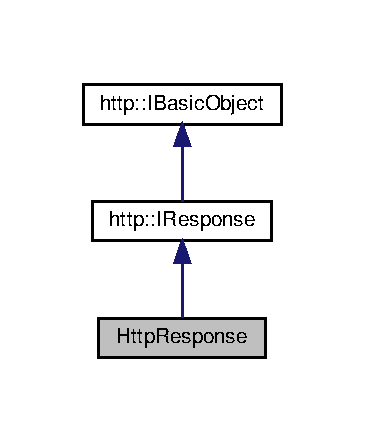
\includegraphics[width=175pt]{classHttpResponse__inherit__graph}
\end{center}
\end{figure}


Collaboration diagram for Http\+Response\+:
\nopagebreak
\begin{figure}[H]
\begin{center}
\leavevmode
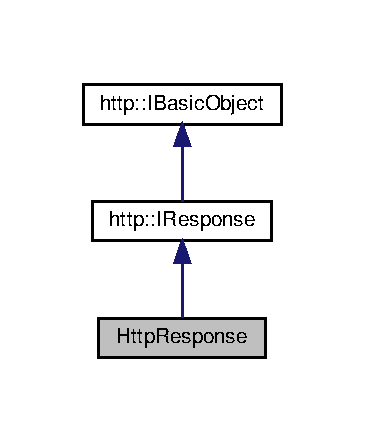
\includegraphics[width=175pt]{classHttpResponse__coll__graph}
\end{center}
\end{figure}
\subsection*{Public Member Functions}
\begin{DoxyCompactItemize}
\item 
\mbox{\Hypertarget{classHttpResponse_a6b135899b9658fda70a4b81b2454382c}\label{classHttpResponse_a6b135899b9658fda70a4b81b2454382c}} 
{\bfseries Http\+Response} (std\+::string response)
\item 
int \hyperlink{classHttpResponse_a5cb28c82fc2f657808b61f0f6bb67f28}{status\+Code} () const noexcept
\begin{DoxyCompactList}\small\item\em Returns the status code of the response. \end{DoxyCompactList}\item 
bool \hyperlink{classHttpResponse_a8a6cc8f27e81ca4d2ef4ec60450974d1}{status\+Code} (int status\+Code) noexcept
\begin{DoxyCompactList}\small\item\em Set the status code of the response. \end{DoxyCompactList}\item 
std\+::string \hyperlink{classHttpResponse_a5463015a6d521c4c4da46505c0740f63}{status\+Message} () const noexcept
\begin{DoxyCompactList}\small\item\em Returns the status message of the response. \end{DoxyCompactList}\item 
bool \hyperlink{classHttpResponse_ad705d5d1846c261e2ca80c24c9e1d75c}{status\+Message} (std\+::string status\+Message) noexcept
\begin{DoxyCompactList}\small\item\em Set the status message of the response. \end{DoxyCompactList}\item 
\mbox{\Hypertarget{classHttpResponse_a2f6f0f1588f9a06c360648cabb6e58e1}\label{classHttpResponse_a2f6f0f1588f9a06c360648cabb6e58e1}} 
bool \hyperlink{classHttpResponse_a2f6f0f1588f9a06c360648cabb6e58e1}{set\+Cookie} (std\+::string name, std\+::string value, Cookie\+Options options=Cookie\+Options()) noexcept
\begin{DoxyCompactList}\small\item\em Return the value of the cookie \textquotesingle{}name\textquotesingle{} In header there are an header parameter name \textquotesingle{}Cookie\textquotesingle{} who has all cookies of the request ex\+: \char`\"{}\+Cookie\+: yummy\+\_\+cookie=choco; tasty\+\_\+cookie=strawberry\char`\"{} He can have options like Expires, Domain, Max-\/\+Age, ... Return false if the name or the value are invalids. \end{DoxyCompactList}\item 
\mbox{\Hypertarget{classHttpResponse_a1fde59ad363da86edb45efc6b7844e64}\label{classHttpResponse_a1fde59ad363da86edb45efc6b7844e64}} 
std\+::string \hyperlink{classHttpResponse_a1fde59ad363da86edb45efc6b7844e64}{protocol} () const noexcept
\begin{DoxyCompactList}\small\item\em Return the protocol of the object. \end{DoxyCompactList}\item 
bool \hyperlink{classHttpResponse_ae119bd9c54b39e392b2fd87c3012f53e}{header\+Parameter\+Exist} (const std\+::string \&key) const noexcept
\begin{DoxyCompactList}\small\item\em Checks if in object, there are a named \textquotesingle{}key\textquotesingle{} header parameter. \end{DoxyCompactList}\item 
std\+::string \hyperlink{classHttpResponse_a257c44a876f78e131e32d5af9f81d4fc}{header\+Parameter} (const std\+::string \&key) const noexcept
\begin{DoxyCompactList}\small\item\em Return the header parameter \char`\"{}key\char`\"{} found in the object. \end{DoxyCompactList}\item 
bool \hyperlink{classHttpResponse_a193cf7b72bfedfc7f37318aff1d55158}{header\+Parameter} (std\+::string key, std\+::string value) noexcept
\begin{DoxyCompactList}\small\item\em Add / Update a header parameter. \end{DoxyCompactList}\item 
std\+::string \hyperlink{classHttpResponse_a696715c993a4ec50a609efcd43d98a62}{body} () const noexcept
\begin{DoxyCompactList}\small\item\em Return the body of the object. \end{DoxyCompactList}\item 
bool \hyperlink{classHttpResponse_a26f66b018b250a0ee37859730e131404}{body} (std\+::string body) noexcept
\begin{DoxyCompactList}\small\item\em Set / Add a new body in the object. \end{DoxyCompactList}\item 
bool \hyperlink{classHttpResponse_af8f8669568d6bcc7b0e3c7a247e456bd}{body\+Append} (std\+::string \hyperlink{classHttpResponse_a696715c993a4ec50a609efcd43d98a62}{body}) noexcept
\begin{DoxyCompactList}\small\item\em Append data in the body or create it if not exist. \end{DoxyCompactList}\item 
\mbox{\Hypertarget{classHttpResponse_aad0171e5838c46a14c562d4cfe771f4e}\label{classHttpResponse_aad0171e5838c46a14c562d4cfe771f4e}} 
std\+::string \hyperlink{classHttpResponse_aad0171e5838c46a14c562d4cfe771f4e}{serialize} () const noexcept
\begin{DoxyCompactList}\small\item\em Transform this object in a true http object. \end{DoxyCompactList}\end{DoxyCompactItemize}


\subsection{Member Function Documentation}
\mbox{\Hypertarget{classHttpResponse_a696715c993a4ec50a609efcd43d98a62}\label{classHttpResponse_a696715c993a4ec50a609efcd43d98a62}} 
\index{Http\+Response@{Http\+Response}!body@{body}}
\index{body@{body}!Http\+Response@{Http\+Response}}
\subsubsection{\texorpdfstring{body()}{body()}\hspace{0.1cm}{\footnotesize\ttfamily [1/2]}}
{\footnotesize\ttfamily std\+::string Http\+Response\+::body (\begin{DoxyParamCaption}{ }\end{DoxyParamCaption}) const\hspace{0.3cm}{\ttfamily [virtual]}, {\ttfamily [noexcept]}}



Return the body of the object. 

Sometimes in object like P\+O\+ST there are a body He can take any form (json, form-\/url-\/encoded, xml, plain text, ...) 

Implements \hyperlink{structhttp_1_1IBasicObject_a42eda0e62758f23d9d7d1fee01d8747a}{http\+::\+I\+Basic\+Object}.

\mbox{\Hypertarget{classHttpResponse_a26f66b018b250a0ee37859730e131404}\label{classHttpResponse_a26f66b018b250a0ee37859730e131404}} 
\index{Http\+Response@{Http\+Response}!body@{body}}
\index{body@{body}!Http\+Response@{Http\+Response}}
\subsubsection{\texorpdfstring{body()}{body()}\hspace{0.1cm}{\footnotesize\ttfamily [2/2]}}
{\footnotesize\ttfamily bool Http\+Response\+::body (\begin{DoxyParamCaption}\item[{std\+::string}]{body }\end{DoxyParamCaption})\hspace{0.3cm}{\ttfamily [virtual]}, {\ttfamily [noexcept]}}



Set / Add a new body in the object. 

Sometimes in object like P\+O\+ST there are a body He can take any form (json, form-\/url-\/encoded, xml, plain text, ...) Change / Add the \textquotesingle{}Content-\/\+Length\textquotesingle{} header parameter Return false if the body is empty or too large... 

Implements \hyperlink{structhttp_1_1IBasicObject_aa304f3a3137912f1dbff798531fa4c09}{http\+::\+I\+Basic\+Object}.

\mbox{\Hypertarget{classHttpResponse_af8f8669568d6bcc7b0e3c7a247e456bd}\label{classHttpResponse_af8f8669568d6bcc7b0e3c7a247e456bd}} 
\index{Http\+Response@{Http\+Response}!body\+Append@{body\+Append}}
\index{body\+Append@{body\+Append}!Http\+Response@{Http\+Response}}
\subsubsection{\texorpdfstring{body\+Append()}{bodyAppend()}}
{\footnotesize\ttfamily bool Http\+Response\+::body\+Append (\begin{DoxyParamCaption}\item[{std\+::string}]{body }\end{DoxyParamCaption})\hspace{0.3cm}{\ttfamily [virtual]}, {\ttfamily [noexcept]}}



Append data in the body or create it if not exist. 

Sometimes in object like P\+O\+ST there are a body He can take any form (json, form-\/url-\/encoded, xml, plain text, ...) Change / Add the \textquotesingle{}Content-\/\+Length\textquotesingle{} header parameter Return false if the body is empty or too large... 

Implements \hyperlink{structhttp_1_1IBasicObject_abf2cb4a0e7908313b827ad4635bad730}{http\+::\+I\+Basic\+Object}.

\mbox{\Hypertarget{classHttpResponse_a257c44a876f78e131e32d5af9f81d4fc}\label{classHttpResponse_a257c44a876f78e131e32d5af9f81d4fc}} 
\index{Http\+Response@{Http\+Response}!header\+Parameter@{header\+Parameter}}
\index{header\+Parameter@{header\+Parameter}!Http\+Response@{Http\+Response}}
\subsubsection{\texorpdfstring{header\+Parameter()}{headerParameter()}\hspace{0.1cm}{\footnotesize\ttfamily [1/2]}}
{\footnotesize\ttfamily std\+::string Http\+Response\+::header\+Parameter (\begin{DoxyParamCaption}\item[{const std\+::string \&}]{key }\end{DoxyParamCaption}) const\hspace{0.3cm}{\ttfamily [virtual]}, {\ttfamily [noexcept]}}



Return the header parameter \char`\"{}key\char`\"{} found in the object. 

In http object there are some header parameters like \char`\"{}\+Content-\/\+Lenght\+: 166\char`\"{}, \char`\"{}host\+: localhost\char`\"{}. They are described by \char`\"{}\{\+K\+E\+Y\}\+: \{\+V\+A\+L\+U\+E\}\char`\"{} Return an empty string if the parameters key not exist 

Implements \hyperlink{structhttp_1_1IBasicObject_a17f97dd4917fdd7dd694d3d191eaebca}{http\+::\+I\+Basic\+Object}.

\mbox{\Hypertarget{classHttpResponse_a193cf7b72bfedfc7f37318aff1d55158}\label{classHttpResponse_a193cf7b72bfedfc7f37318aff1d55158}} 
\index{Http\+Response@{Http\+Response}!header\+Parameter@{header\+Parameter}}
\index{header\+Parameter@{header\+Parameter}!Http\+Response@{Http\+Response}}
\subsubsection{\texorpdfstring{header\+Parameter()}{headerParameter()}\hspace{0.1cm}{\footnotesize\ttfamily [2/2]}}
{\footnotesize\ttfamily bool Http\+Response\+::header\+Parameter (\begin{DoxyParamCaption}\item[{std\+::string}]{key,  }\item[{std\+::string}]{value }\end{DoxyParamCaption})\hspace{0.3cm}{\ttfamily [virtual]}, {\ttfamily [noexcept]}}



Add / Update a header parameter. 

In http object there are some header parameters like \char`\"{}\+Content-\/\+Lenght\+: 166\char`\"{}, \char`\"{}host\+: localhost\char`\"{}. They are described by \char`\"{}\{\+K\+E\+Y\}\+: \{\+V\+A\+L\+U\+E\}\char`\"{} Return false if the key or value aren\textquotesingle{}t valid 

Implements \hyperlink{structhttp_1_1IBasicObject_a0d1fff270c6069bedf87e86cdac6bf3d}{http\+::\+I\+Basic\+Object}.

\mbox{\Hypertarget{classHttpResponse_ae119bd9c54b39e392b2fd87c3012f53e}\label{classHttpResponse_ae119bd9c54b39e392b2fd87c3012f53e}} 
\index{Http\+Response@{Http\+Response}!header\+Parameter\+Exist@{header\+Parameter\+Exist}}
\index{header\+Parameter\+Exist@{header\+Parameter\+Exist}!Http\+Response@{Http\+Response}}
\subsubsection{\texorpdfstring{header\+Parameter\+Exist()}{headerParameterExist()}}
{\footnotesize\ttfamily bool Http\+Response\+::header\+Parameter\+Exist (\begin{DoxyParamCaption}\item[{const std\+::string \&}]{key }\end{DoxyParamCaption}) const\hspace{0.3cm}{\ttfamily [virtual]}, {\ttfamily [noexcept]}}



Checks if in object, there are a named \textquotesingle{}key\textquotesingle{} header parameter. 

In http object there are some header parameters like \char`\"{}\+Content-\/\+Lenght\+: 166\char`\"{}, \char`\"{}host\+: localhost\char`\"{}. They are described by \char`\"{}\{\+K\+E\+Y\}\+: \{\+V\+A\+L\+U\+E\}\char`\"{} 

Implements \hyperlink{structhttp_1_1IBasicObject_a581e48c03a666b87082c75427f0ff835}{http\+::\+I\+Basic\+Object}.

\mbox{\Hypertarget{classHttpResponse_a5cb28c82fc2f657808b61f0f6bb67f28}\label{classHttpResponse_a5cb28c82fc2f657808b61f0f6bb67f28}} 
\index{Http\+Response@{Http\+Response}!status\+Code@{status\+Code}}
\index{status\+Code@{status\+Code}!Http\+Response@{Http\+Response}}
\subsubsection{\texorpdfstring{status\+Code()}{statusCode()}\hspace{0.1cm}{\footnotesize\ttfamily [1/2]}}
{\footnotesize\ttfamily int Http\+Response\+::status\+Code (\begin{DoxyParamCaption}{ }\end{DoxyParamCaption}) const\hspace{0.3cm}{\ttfamily [virtual]}, {\ttfamily [noexcept]}}



Returns the status code of the response. 

In http response there are always status code like 200 or 404 To describe if the request is executed correctly 

Implements \hyperlink{structhttp_1_1IResponse_ad980a7a0b5f1de80bd1faa84706e922f}{http\+::\+I\+Response}.

\mbox{\Hypertarget{classHttpResponse_a8a6cc8f27e81ca4d2ef4ec60450974d1}\label{classHttpResponse_a8a6cc8f27e81ca4d2ef4ec60450974d1}} 
\index{Http\+Response@{Http\+Response}!status\+Code@{status\+Code}}
\index{status\+Code@{status\+Code}!Http\+Response@{Http\+Response}}
\subsubsection{\texorpdfstring{status\+Code()}{statusCode()}\hspace{0.1cm}{\footnotesize\ttfamily [2/2]}}
{\footnotesize\ttfamily bool Http\+Response\+::status\+Code (\begin{DoxyParamCaption}\item[{int}]{status\+Code }\end{DoxyParamCaption})\hspace{0.3cm}{\ttfamily [virtual]}, {\ttfamily [noexcept]}}



Set the status code of the response. 

In http response there are always status code like \char`\"{}200\char`\"{} or \char`\"{}404\char`\"{} To describe if the request is executed correctly Return false if the status code isn\textquotesingle{}t valid 

Implements \hyperlink{structhttp_1_1IResponse_a7d85b2b27acb82d13cf26eb0d3801735}{http\+::\+I\+Response}.

\mbox{\Hypertarget{classHttpResponse_a5463015a6d521c4c4da46505c0740f63}\label{classHttpResponse_a5463015a6d521c4c4da46505c0740f63}} 
\index{Http\+Response@{Http\+Response}!status\+Message@{status\+Message}}
\index{status\+Message@{status\+Message}!Http\+Response@{Http\+Response}}
\subsubsection{\texorpdfstring{status\+Message()}{statusMessage()}\hspace{0.1cm}{\footnotesize\ttfamily [1/2]}}
{\footnotesize\ttfamily std\+::string Http\+Response\+::status\+Message (\begin{DoxyParamCaption}{ }\end{DoxyParamCaption}) const\hspace{0.3cm}{\ttfamily [virtual]}, {\ttfamily [noexcept]}}



Returns the status message of the response. 

In http response there are always status message after the status code like \char`\"{}200 O\+K\char`\"{} or \char`\"{}404 Not found\char`\"{} 

Implements \hyperlink{structhttp_1_1IResponse_a4339fd29b105c9ea5319b2e01f27290c}{http\+::\+I\+Response}.

\mbox{\Hypertarget{classHttpResponse_ad705d5d1846c261e2ca80c24c9e1d75c}\label{classHttpResponse_ad705d5d1846c261e2ca80c24c9e1d75c}} 
\index{Http\+Response@{Http\+Response}!status\+Message@{status\+Message}}
\index{status\+Message@{status\+Message}!Http\+Response@{Http\+Response}}
\subsubsection{\texorpdfstring{status\+Message()}{statusMessage()}\hspace{0.1cm}{\footnotesize\ttfamily [2/2]}}
{\footnotesize\ttfamily bool Http\+Response\+::status\+Message (\begin{DoxyParamCaption}\item[{std\+::string}]{status\+Message }\end{DoxyParamCaption})\hspace{0.3cm}{\ttfamily [virtual]}, {\ttfamily [noexcept]}}



Set the status message of the response. 

In http response there are always status message after the status code like \char`\"{}200 O\+K\char`\"{} or \char`\"{}404 Not found\char`\"{} Return false if the status message isn\textquotesingle{}t valid 

Implements \hyperlink{structhttp_1_1IResponse_ae2a223c2d714b456f2a064e13cafc2e2}{http\+::\+I\+Response}.



The documentation for this class was generated from the following files\+:\begin{DoxyCompactItemize}
\item 
inc/\+Core/\+Http/Http\+Response.\+hpp\item 
src/\+Core/\+Http/Http\+Response.\+cpp\end{DoxyCompactItemize}

\hypertarget{structhttp_1_1IBasicObject}{}\section{http\+:\+:I\+Basic\+Object Struct Reference}
\label{structhttp_1_1IBasicObject}\index{http\+::\+I\+Basic\+Object@{http\+::\+I\+Basic\+Object}}


\href{http::IBasicObject}{\tt http\+::\+I\+Basic\+Object} is a interface that describe same object in a http request / response  




{\ttfamily \#include $<$I\+Basic\+Object.\+hpp$>$}



Inheritance diagram for http\+:\+:I\+Basic\+Object\+:
\nopagebreak
\begin{figure}[H]
\begin{center}
\leavevmode
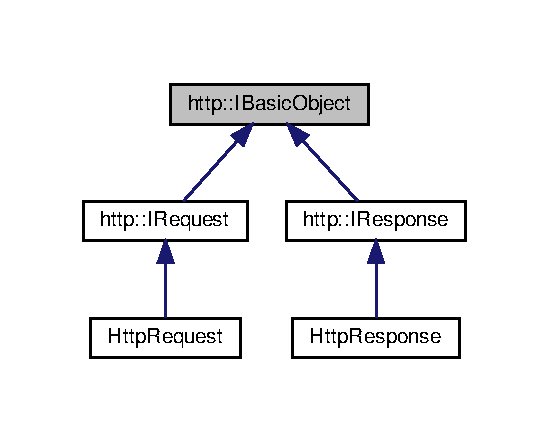
\includegraphics[width=264pt]{structhttp_1_1IBasicObject__inherit__graph}
\end{center}
\end{figure}
\subsection*{Public Member Functions}
\begin{DoxyCompactItemize}
\item 
\mbox{\Hypertarget{structhttp_1_1IBasicObject_ab605c64288bb38ef22741ee5ae1d1f41}\label{structhttp_1_1IBasicObject_ab605c64288bb38ef22741ee5ae1d1f41}} 
virtual \hyperlink{structhttp_1_1IBasicObject_ab605c64288bb38ef22741ee5ae1d1f41}{$\sim$\+I\+Basic\+Object} ()=default
\begin{DoxyCompactList}\small\item\em Default destructor. \end{DoxyCompactList}\item 
\mbox{\Hypertarget{structhttp_1_1IBasicObject_a691aac60028d3b8785b80bfff286c51a}\label{structhttp_1_1IBasicObject_a691aac60028d3b8785b80bfff286c51a}} 
virtual std\+::string \hyperlink{structhttp_1_1IBasicObject_a691aac60028d3b8785b80bfff286c51a}{protocol} () const noexcept=0
\begin{DoxyCompactList}\small\item\em Return the protocol of the object. \end{DoxyCompactList}\item 
virtual bool \hyperlink{structhttp_1_1IBasicObject_a581e48c03a666b87082c75427f0ff835}{header\+Parameter\+Exist} (const std\+::string \&key) const noexcept=0
\begin{DoxyCompactList}\small\item\em Checks if in object, there are a named \textquotesingle{}key\textquotesingle{} header parameter. \end{DoxyCompactList}\item 
virtual std\+::string \hyperlink{structhttp_1_1IBasicObject_a17f97dd4917fdd7dd694d3d191eaebca}{header\+Parameter} (const std\+::string \&key) const noexcept=0
\begin{DoxyCompactList}\small\item\em Return the header parameter \char`\"{}key\char`\"{} found in the object. \end{DoxyCompactList}\item 
virtual bool \hyperlink{structhttp_1_1IBasicObject_a0d1fff270c6069bedf87e86cdac6bf3d}{header\+Parameter} (std\+::string key, std\+::string value) noexcept=0
\begin{DoxyCompactList}\small\item\em Add / Update a header parameter. \end{DoxyCompactList}\item 
virtual std\+::string \hyperlink{structhttp_1_1IBasicObject_a42eda0e62758f23d9d7d1fee01d8747a}{body} () const noexcept=0
\begin{DoxyCompactList}\small\item\em Return the body of the object. \end{DoxyCompactList}\item 
virtual bool \hyperlink{structhttp_1_1IBasicObject_aa304f3a3137912f1dbff798531fa4c09}{body} (std\+::string body) noexcept=0
\begin{DoxyCompactList}\small\item\em Set / Add a new body in the object. \end{DoxyCompactList}\item 
virtual bool \hyperlink{structhttp_1_1IBasicObject_abf2cb4a0e7908313b827ad4635bad730}{body\+Append} (std\+::string \hyperlink{structhttp_1_1IBasicObject_a42eda0e62758f23d9d7d1fee01d8747a}{body}) noexcept=0
\begin{DoxyCompactList}\small\item\em Append data in the body or create it if not exist. \end{DoxyCompactList}\item 
\mbox{\Hypertarget{structhttp_1_1IBasicObject_a2d7945a7f4c4e38ce29525bb17c8a5a5}\label{structhttp_1_1IBasicObject_a2d7945a7f4c4e38ce29525bb17c8a5a5}} 
virtual std\+::string \hyperlink{structhttp_1_1IBasicObject_a2d7945a7f4c4e38ce29525bb17c8a5a5}{serialize} () const noexcept=0
\begin{DoxyCompactList}\small\item\em Transform this object in a true http object. \end{DoxyCompactList}\end{DoxyCompactItemize}


\subsection{Detailed Description}
\href{http::IBasicObject}{\tt http\+::\+I\+Basic\+Object} is a interface that describe same object in a http request / response 

\subsection{Member Function Documentation}
\mbox{\Hypertarget{structhttp_1_1IBasicObject_a42eda0e62758f23d9d7d1fee01d8747a}\label{structhttp_1_1IBasicObject_a42eda0e62758f23d9d7d1fee01d8747a}} 
\index{http\+::\+I\+Basic\+Object@{http\+::\+I\+Basic\+Object}!body@{body}}
\index{body@{body}!http\+::\+I\+Basic\+Object@{http\+::\+I\+Basic\+Object}}
\subsubsection{\texorpdfstring{body()}{body()}\hspace{0.1cm}{\footnotesize\ttfamily [1/2]}}
{\footnotesize\ttfamily virtual std\+::string http\+::\+I\+Basic\+Object\+::body (\begin{DoxyParamCaption}{ }\end{DoxyParamCaption}) const\hspace{0.3cm}{\ttfamily [pure virtual]}, {\ttfamily [noexcept]}}



Return the body of the object. 

Sometimes in object like P\+O\+ST there are a body He can take any form (json, form-\/url-\/encoded, xml, plain text, ...) 

Implemented in \hyperlink{classHttpRequest_a16be46a53c2d2f8d29ad89aa213f30bb}{Http\+Request}, and \hyperlink{classHttpResponse_a696715c993a4ec50a609efcd43d98a62}{Http\+Response}.

\mbox{\Hypertarget{structhttp_1_1IBasicObject_aa304f3a3137912f1dbff798531fa4c09}\label{structhttp_1_1IBasicObject_aa304f3a3137912f1dbff798531fa4c09}} 
\index{http\+::\+I\+Basic\+Object@{http\+::\+I\+Basic\+Object}!body@{body}}
\index{body@{body}!http\+::\+I\+Basic\+Object@{http\+::\+I\+Basic\+Object}}
\subsubsection{\texorpdfstring{body()}{body()}\hspace{0.1cm}{\footnotesize\ttfamily [2/2]}}
{\footnotesize\ttfamily virtual bool http\+::\+I\+Basic\+Object\+::body (\begin{DoxyParamCaption}\item[{std\+::string}]{body }\end{DoxyParamCaption})\hspace{0.3cm}{\ttfamily [pure virtual]}, {\ttfamily [noexcept]}}



Set / Add a new body in the object. 

Sometimes in object like P\+O\+ST there are a body He can take any form (json, form-\/url-\/encoded, xml, plain text, ...) Change / Add the \textquotesingle{}Content-\/\+Length\textquotesingle{} header parameter Return false if the body is empty or too large... 

Implemented in \hyperlink{classHttpRequest_a591fb5ec9430764ed5b3578d49c3858f}{Http\+Request}, and \hyperlink{classHttpResponse_a26f66b018b250a0ee37859730e131404}{Http\+Response}.

\mbox{\Hypertarget{structhttp_1_1IBasicObject_abf2cb4a0e7908313b827ad4635bad730}\label{structhttp_1_1IBasicObject_abf2cb4a0e7908313b827ad4635bad730}} 
\index{http\+::\+I\+Basic\+Object@{http\+::\+I\+Basic\+Object}!body\+Append@{body\+Append}}
\index{body\+Append@{body\+Append}!http\+::\+I\+Basic\+Object@{http\+::\+I\+Basic\+Object}}
\subsubsection{\texorpdfstring{body\+Append()}{bodyAppend()}}
{\footnotesize\ttfamily virtual bool http\+::\+I\+Basic\+Object\+::body\+Append (\begin{DoxyParamCaption}\item[{std\+::string}]{body }\end{DoxyParamCaption})\hspace{0.3cm}{\ttfamily [pure virtual]}, {\ttfamily [noexcept]}}



Append data in the body or create it if not exist. 

Sometimes in object like P\+O\+ST there are a body He can take any form (json, form-\/url-\/encoded, xml, plain text, ...) Change / Add the \textquotesingle{}Content-\/\+Length\textquotesingle{} header parameter Return false if the body is empty or too large... 

Implemented in \hyperlink{classHttpRequest_afd8f9f22651d2844b7b2d4cb882b7e19}{Http\+Request}, and \hyperlink{classHttpResponse_af8f8669568d6bcc7b0e3c7a247e456bd}{Http\+Response}.

\mbox{\Hypertarget{structhttp_1_1IBasicObject_a17f97dd4917fdd7dd694d3d191eaebca}\label{structhttp_1_1IBasicObject_a17f97dd4917fdd7dd694d3d191eaebca}} 
\index{http\+::\+I\+Basic\+Object@{http\+::\+I\+Basic\+Object}!header\+Parameter@{header\+Parameter}}
\index{header\+Parameter@{header\+Parameter}!http\+::\+I\+Basic\+Object@{http\+::\+I\+Basic\+Object}}
\subsubsection{\texorpdfstring{header\+Parameter()}{headerParameter()}\hspace{0.1cm}{\footnotesize\ttfamily [1/2]}}
{\footnotesize\ttfamily virtual std\+::string http\+::\+I\+Basic\+Object\+::header\+Parameter (\begin{DoxyParamCaption}\item[{const std\+::string \&}]{key }\end{DoxyParamCaption}) const\hspace{0.3cm}{\ttfamily [pure virtual]}, {\ttfamily [noexcept]}}



Return the header parameter \char`\"{}key\char`\"{} found in the object. 

In http object there are some header parameters like \char`\"{}\+Content-\/\+Lenght\+: 166\char`\"{}, \char`\"{}host\+: localhost\char`\"{}. They are described by \char`\"{}\{\+K\+E\+Y\}\+: \{\+V\+A\+L\+U\+E\}\char`\"{} Return an empty string if the parameters key not exist 

Implemented in \hyperlink{classHttpRequest_a96f232879fff933182a3ed5c80229df6}{Http\+Request}, and \hyperlink{classHttpResponse_a257c44a876f78e131e32d5af9f81d4fc}{Http\+Response}.

\mbox{\Hypertarget{structhttp_1_1IBasicObject_a0d1fff270c6069bedf87e86cdac6bf3d}\label{structhttp_1_1IBasicObject_a0d1fff270c6069bedf87e86cdac6bf3d}} 
\index{http\+::\+I\+Basic\+Object@{http\+::\+I\+Basic\+Object}!header\+Parameter@{header\+Parameter}}
\index{header\+Parameter@{header\+Parameter}!http\+::\+I\+Basic\+Object@{http\+::\+I\+Basic\+Object}}
\subsubsection{\texorpdfstring{header\+Parameter()}{headerParameter()}\hspace{0.1cm}{\footnotesize\ttfamily [2/2]}}
{\footnotesize\ttfamily virtual bool http\+::\+I\+Basic\+Object\+::header\+Parameter (\begin{DoxyParamCaption}\item[{std\+::string}]{key,  }\item[{std\+::string}]{value }\end{DoxyParamCaption})\hspace{0.3cm}{\ttfamily [pure virtual]}, {\ttfamily [noexcept]}}



Add / Update a header parameter. 

In http object there are some header parameters like \char`\"{}\+Content-\/\+Lenght\+: 166\char`\"{}, \char`\"{}host\+: localhost\char`\"{}. They are described by \char`\"{}\{\+K\+E\+Y\}\+: \{\+V\+A\+L\+U\+E\}\char`\"{} Return false if the key or value aren\textquotesingle{}t valid 

Implemented in \hyperlink{classHttpRequest_a04f974104da7c06c568a8e648693e92c}{Http\+Request}, and \hyperlink{classHttpResponse_a193cf7b72bfedfc7f37318aff1d55158}{Http\+Response}.

\mbox{\Hypertarget{structhttp_1_1IBasicObject_a581e48c03a666b87082c75427f0ff835}\label{structhttp_1_1IBasicObject_a581e48c03a666b87082c75427f0ff835}} 
\index{http\+::\+I\+Basic\+Object@{http\+::\+I\+Basic\+Object}!header\+Parameter\+Exist@{header\+Parameter\+Exist}}
\index{header\+Parameter\+Exist@{header\+Parameter\+Exist}!http\+::\+I\+Basic\+Object@{http\+::\+I\+Basic\+Object}}
\subsubsection{\texorpdfstring{header\+Parameter\+Exist()}{headerParameterExist()}}
{\footnotesize\ttfamily virtual bool http\+::\+I\+Basic\+Object\+::header\+Parameter\+Exist (\begin{DoxyParamCaption}\item[{const std\+::string \&}]{key }\end{DoxyParamCaption}) const\hspace{0.3cm}{\ttfamily [pure virtual]}, {\ttfamily [noexcept]}}



Checks if in object, there are a named \textquotesingle{}key\textquotesingle{} header parameter. 

In http object there are some header parameters like \char`\"{}\+Content-\/\+Lenght\+: 166\char`\"{}, \char`\"{}host\+: localhost\char`\"{}. They are described by \char`\"{}\{\+K\+E\+Y\}\+: \{\+V\+A\+L\+U\+E\}\char`\"{} 

Implemented in \hyperlink{classHttpRequest_a74ea75d8685647989346bd5d1d25702a}{Http\+Request}, and \hyperlink{classHttpResponse_ae119bd9c54b39e392b2fd87c3012f53e}{Http\+Response}.



The documentation for this struct was generated from the following file\+:\begin{DoxyCompactItemize}
\item 
inc/\+Core/\+Http/api/I\+Basic\+Object.\+hpp\end{DoxyCompactItemize}

\hypertarget{structnet_1_1IClient}{}\section{net\+:\+:I\+Client Struct Reference}
\label{structnet_1_1IClient}\index{net\+::\+I\+Client@{net\+::\+I\+Client}}


Inheritance diagram for net\+:\+:I\+Client\+:
\nopagebreak
\begin{figure}[H]
\begin{center}
\leavevmode
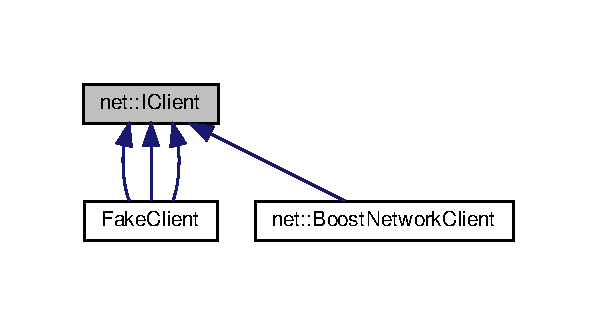
\includegraphics[width=287pt]{structnet_1_1IClient__inherit__graph}
\end{center}
\end{figure}
\subsection*{Public Member Functions}
\begin{DoxyCompactItemize}
\item 
\mbox{\Hypertarget{structnet_1_1IClient_a0af7b8c2c794bb59fb469805e6fe9782}\label{structnet_1_1IClient_a0af7b8c2c794bb59fb469805e6fe9782}} 
virtual \hyperlink{structnet_1_1IClient_a0af7b8c2c794bb59fb469805e6fe9782}{$\sim$\+I\+Client} ()=default
\begin{DoxyCompactList}\small\item\em Default destructor. \end{DoxyCompactList}\item 
virtual bool \hyperlink{structnet_1_1IClient_a44691ffe41185a41b5637d7c0068b5f2}{send} (const std\+::string \&data)=0
\begin{DoxyCompactList}\small\item\em Send \textquotesingle{}data\textquotesingle{} into a tcp packet to the client. \end{DoxyCompactList}\item 
\mbox{\Hypertarget{structnet_1_1IClient_a3233d8ad9276c621e3545c8afce8be42}\label{structnet_1_1IClient_a3233d8ad9276c621e3545c8afce8be42}} 
virtual std\+::size\+\_\+t \hyperlink{structnet_1_1IClient_a3233d8ad9276c621e3545c8afce8be42}{get\+Id} () const noexcept=0
\begin{DoxyCompactList}\small\item\em Gets an unique ID on the client. \end{DoxyCompactList}\end{DoxyCompactItemize}


\subsection{Member Function Documentation}
\mbox{\Hypertarget{structnet_1_1IClient_a44691ffe41185a41b5637d7c0068b5f2}\label{structnet_1_1IClient_a44691ffe41185a41b5637d7c0068b5f2}} 
\index{net\+::\+I\+Client@{net\+::\+I\+Client}!send@{send}}
\index{send@{send}!net\+::\+I\+Client@{net\+::\+I\+Client}}
\subsubsection{\texorpdfstring{send()}{send()}}
{\footnotesize\ttfamily virtual bool net\+::\+I\+Client\+::send (\begin{DoxyParamCaption}\item[{const std\+::string \&}]{data }\end{DoxyParamCaption})\hspace{0.3cm}{\ttfamily [pure virtual]}}



Send \textquotesingle{}data\textquotesingle{} into a tcp packet to the client. 

Return true if there are no problems 

Implemented in \hyperlink{classnet_1_1BoostNetworkClient_af584270d274c31b315eba24effd86b46}{net\+::\+Boost\+Network\+Client}.



The documentation for this struct was generated from the following file\+:\begin{DoxyCompactItemize}
\item 
inc/\+Network/I\+Client.\+hpp\end{DoxyCompactItemize}

\hypertarget{classIConfigNode}{}\section{I\+Config\+Node Class Reference}
\label{classIConfigNode}\index{I\+Config\+Node@{I\+Config\+Node}}


Inheritance diagram for I\+Config\+Node\+:
\nopagebreak
\begin{figure}[H]
\begin{center}
\leavevmode
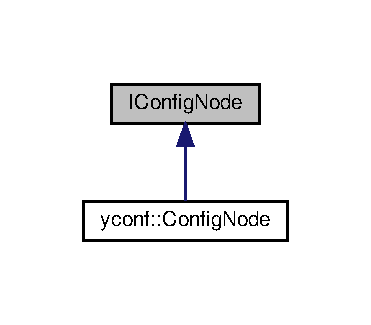
\includegraphics[width=178pt]{classIConfigNode__inherit__graph}
\end{center}
\end{figure}
\subsection*{Public Member Functions}
\begin{DoxyCompactItemize}
\item 
virtual std\+::unique\+\_\+ptr$<$ \hyperlink{classIConfigNode}{I\+Config\+Node} $>$ \hyperlink{classIConfigNode_a113e74aac6e8c62f5d5762b766f934e6}{get\+Child} (const std\+::string \&name) const =0
\begin{DoxyCompactList}\small\item\em Gets a child node. \end{DoxyCompactList}\item 
virtual std\+::string \hyperlink{classIConfigNode_ae32a49d812d3f98cbc048ab3cce5f7d6}{get\+Value} (const std\+::string \&name) const =0
\begin{DoxyCompactList}\small\item\em Gets the value of a property. \end{DoxyCompactList}\item 
virtual std\+::vector$<$ std\+::string $>$ \hyperlink{classIConfigNode_aaa66c9d23d521b5b5c9f5f6bf35087fb}{get\+Scalar\+Array} (const std\+::string \&name) const =0
\begin{DoxyCompactList}\small\item\em Gets the content of the array, as scalars. \end{DoxyCompactList}\item 
virtual std\+::vector$<$ std\+::unique\+\_\+ptr$<$ \hyperlink{classIConfigNode}{I\+Config\+Node} $>$ $>$ \hyperlink{classIConfigNode_a3a15562e0598f5bb105ddd006e298157}{get\+Node\+Array} (const std\+::string \&name) const =0
\begin{DoxyCompactList}\small\item\em Gets the content of the array, as nodes. \end{DoxyCompactList}\item 
virtual std\+::unordered\+\_\+map$<$ std\+::string, std\+::string $>$ \hyperlink{classIConfigNode_ae6abd34301fc7141963ef125117db0c5}{get\+All\+Scalars\+Of} (const std\+::string \&name) const =0
\begin{DoxyCompactList}\small\item\em Returns all the properties from the node. \end{DoxyCompactList}\end{DoxyCompactItemize}


\subsection{Member Function Documentation}
\mbox{\Hypertarget{classIConfigNode_ae6abd34301fc7141963ef125117db0c5}\label{classIConfigNode_ae6abd34301fc7141963ef125117db0c5}} 
\index{I\+Config\+Node@{I\+Config\+Node}!get\+All\+Scalars\+Of@{get\+All\+Scalars\+Of}}
\index{get\+All\+Scalars\+Of@{get\+All\+Scalars\+Of}!I\+Config\+Node@{I\+Config\+Node}}
\subsubsection{\texorpdfstring{get\+All\+Scalars\+Of()}{getAllScalarsOf()}}
{\footnotesize\ttfamily virtual std\+::unordered\+\_\+map$<$std\+::string, std\+::string$>$ I\+Config\+Node\+::get\+All\+Scalars\+Of (\begin{DoxyParamCaption}\item[{const std\+::string \&}]{name }\end{DoxyParamCaption}) const\hspace{0.3cm}{\ttfamily [pure virtual]}}



Returns all the properties from the node. 


\begin{DoxyParams}{Parameters}
{\em name} & The name of the wanted node If the name contains dot ({\ttfamily .}), it will get the child of the child, and so on until the last field that is the value name\\
\hline
\end{DoxyParams}
so {\ttfamily get\+All\+Scalars\+Of(\char`\"{}abc.\+def.\+xyz\char`\"{})} is the same as {\ttfamily get\+Child(\char`\"{}abc.\+def\char`\"{})-\/$>$get\+All\+Scalars\+Of(\char`\"{}xyz\char`\"{})}


\begin{DoxyExceptions}{Exceptions}
{\em $<$tt$>$std\+::out\+\_\+of\+\_\+range$<$/tt$>$} & if no such property exists \\
\hline
\end{DoxyExceptions}


Implemented in \hyperlink{classyconf_1_1ConfigNode_af15d6504faf3cf1be0aa5efc5603035f}{yconf\+::\+Config\+Node}.

\mbox{\Hypertarget{classIConfigNode_a113e74aac6e8c62f5d5762b766f934e6}\label{classIConfigNode_a113e74aac6e8c62f5d5762b766f934e6}} 
\index{I\+Config\+Node@{I\+Config\+Node}!get\+Child@{get\+Child}}
\index{get\+Child@{get\+Child}!I\+Config\+Node@{I\+Config\+Node}}
\subsubsection{\texorpdfstring{get\+Child()}{getChild()}}
{\footnotesize\ttfamily virtual std\+::unique\+\_\+ptr$<$\hyperlink{classIConfigNode}{I\+Config\+Node}$>$ I\+Config\+Node\+::get\+Child (\begin{DoxyParamCaption}\item[{const std\+::string \&}]{name }\end{DoxyParamCaption}) const\hspace{0.3cm}{\ttfamily [pure virtual]}}



Gets a child node. 


\begin{DoxyParams}{Parameters}
{\em name} & Name of the wanted child node If the name contains dot ({\ttfamily .}), it will return the child of the child, and so on\\
\hline
\end{DoxyParams}
so {\ttfamily get\+Child(\char`\"{}abc.\+def.\+xyz\char`\"{})} is the same as {\ttfamily get\+Child(\char`\"{}abc\char`\"{})-\/$>$get\+Child(\char`\"{}def\char`\"{})-\/$>$get\+Child(\char`\"{}xyz\char`\"{})}

\begin{DoxyReturn}{Returns}
unique pointer to the child node 
\end{DoxyReturn}

\begin{DoxyExceptions}{Exceptions}
{\em $<$tt$>$std\+::out\+\_\+of\+\_\+range$<$/tt$>$} & if no such child exists \\
\hline
\end{DoxyExceptions}


Implemented in \hyperlink{classyconf_1_1ConfigNode_a419f3e4e042f7cd0746f83d96977d18e}{yconf\+::\+Config\+Node}.

\mbox{\Hypertarget{classIConfigNode_a3a15562e0598f5bb105ddd006e298157}\label{classIConfigNode_a3a15562e0598f5bb105ddd006e298157}} 
\index{I\+Config\+Node@{I\+Config\+Node}!get\+Node\+Array@{get\+Node\+Array}}
\index{get\+Node\+Array@{get\+Node\+Array}!I\+Config\+Node@{I\+Config\+Node}}
\subsubsection{\texorpdfstring{get\+Node\+Array()}{getNodeArray()}}
{\footnotesize\ttfamily virtual std\+::vector$<$std\+::unique\+\_\+ptr$<$\hyperlink{classIConfigNode}{I\+Config\+Node}$>$ $>$ I\+Config\+Node\+::get\+Node\+Array (\begin{DoxyParamCaption}\item[{const std\+::string \&}]{name }\end{DoxyParamCaption}) const\hspace{0.3cm}{\ttfamily [pure virtual]}}



Gets the content of the array, as nodes. 


\begin{DoxyParams}{Parameters}
{\em name} & The name of the wanted array If the name contains dot ({\ttfamily .}), it will get the child of the child, and so on until the last field that is the value name\\
\hline
\end{DoxyParams}
so {\ttfamily get\+Node\+Array(\char`\"{}abc.\+def.\+xyz\char`\"{})} is the same as {\ttfamily get\+Child(\char`\"{}abc.\+def\char`\"{})-\/$>$get\+Node\+Array(\char`\"{}xyz\char`\"{})}

\begin{DoxyReturn}{Returns}
Array content as nodes 
\end{DoxyReturn}

\begin{DoxyExceptions}{Exceptions}
{\em $<$tt$>$std\+::out\+\_\+of\+\_\+range$<$/tt$>$} & if no such property exists \\
\hline
\end{DoxyExceptions}


Implemented in \hyperlink{classyconf_1_1ConfigNode_a3f590d4507699b6f9a9f3ca336f95255}{yconf\+::\+Config\+Node}.

\mbox{\Hypertarget{classIConfigNode_aaa66c9d23d521b5b5c9f5f6bf35087fb}\label{classIConfigNode_aaa66c9d23d521b5b5c9f5f6bf35087fb}} 
\index{I\+Config\+Node@{I\+Config\+Node}!get\+Scalar\+Array@{get\+Scalar\+Array}}
\index{get\+Scalar\+Array@{get\+Scalar\+Array}!I\+Config\+Node@{I\+Config\+Node}}
\subsubsection{\texorpdfstring{get\+Scalar\+Array()}{getScalarArray()}}
{\footnotesize\ttfamily virtual std\+::vector$<$std\+::string$>$ I\+Config\+Node\+::get\+Scalar\+Array (\begin{DoxyParamCaption}\item[{const std\+::string \&}]{name }\end{DoxyParamCaption}) const\hspace{0.3cm}{\ttfamily [pure virtual]}}



Gets the content of the array, as scalars. 


\begin{DoxyParams}{Parameters}
{\em name} & The name of the wanted array If the name contains dot ({\ttfamily .}), it will get the child of the child, and so on until the last field that is the value name\\
\hline
\end{DoxyParams}
so {\ttfamily get\+Scalar\+Array(\char`\"{}abc.\+def.\+xyz\char`\"{})} is the same as {\ttfamily get\+Child(\char`\"{}abc.\+def\char`\"{})-\/$>$get\+Scalar\+Array(\char`\"{}xyz\char`\"{})}

\begin{DoxyReturn}{Returns}
Array content as scalar 
\end{DoxyReturn}

\begin{DoxyExceptions}{Exceptions}
{\em $<$tt$>$std\+::out\+\_\+of\+\_\+range$<$/tt$>$} & if no such property exists \\
\hline
\end{DoxyExceptions}


Implemented in \hyperlink{classyconf_1_1ConfigNode_a4a1ed4e489687b3f1d4d514dbf57595d}{yconf\+::\+Config\+Node}.

\mbox{\Hypertarget{classIConfigNode_ae32a49d812d3f98cbc048ab3cce5f7d6}\label{classIConfigNode_ae32a49d812d3f98cbc048ab3cce5f7d6}} 
\index{I\+Config\+Node@{I\+Config\+Node}!get\+Value@{get\+Value}}
\index{get\+Value@{get\+Value}!I\+Config\+Node@{I\+Config\+Node}}
\subsubsection{\texorpdfstring{get\+Value()}{getValue()}}
{\footnotesize\ttfamily virtual std\+::string I\+Config\+Node\+::get\+Value (\begin{DoxyParamCaption}\item[{const std\+::string \&}]{name }\end{DoxyParamCaption}) const\hspace{0.3cm}{\ttfamily [pure virtual]}}



Gets the value of a property. 


\begin{DoxyParams}{Parameters}
{\em name} & The name of the wanted property If the name contains dot ({\ttfamily .}), it will get the child of the child, and so on until the last field that is the value name\\
\hline
\end{DoxyParams}
so {\ttfamily get\+Value(\char`\"{}abc.\+def.\+xyz\char`\"{})} is the same as {\ttfamily get\+Child(\char`\"{}abc.\+def\char`\"{})-\/$>$get\+Value(\char`\"{}xyz\char`\"{})}

\begin{DoxyReturn}{Returns}
Property value 
\end{DoxyReturn}

\begin{DoxyExceptions}{Exceptions}
{\em $<$tt$>$std\+::out\+\_\+of\+\_\+range$<$/tt$>$} & if no such property exists \\
\hline
\end{DoxyExceptions}


Implemented in \hyperlink{classyconf_1_1ConfigNode_a4670a614581800cfaef06670ad2a0276}{yconf\+::\+Config\+Node}.



The documentation for this class was generated from the following file\+:\begin{DoxyCompactItemize}
\item 
inc/I\+Config\+Node.\+hpp\end{DoxyCompactItemize}

\hypertarget{classnet_1_1INetworkServer}{}\section{net\+:\+:I\+Network\+Server Class Reference}
\label{classnet_1_1INetworkServer}\index{net\+::\+I\+Network\+Server@{net\+::\+I\+Network\+Server}}


Inheritance diagram for net\+:\+:I\+Network\+Server\+:
\nopagebreak
\begin{figure}[H]
\begin{center}
\leavevmode
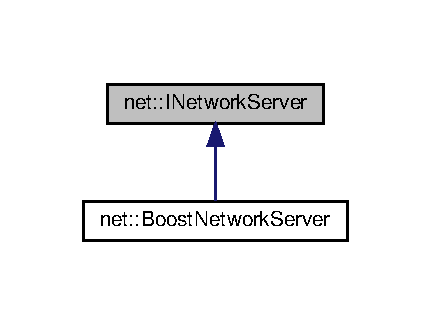
\includegraphics[width=207pt]{classnet_1_1INetworkServer__inherit__graph}
\end{center}
\end{figure}
\subsection*{Public Member Functions}
\begin{DoxyCompactItemize}
\item 
\mbox{\Hypertarget{classnet_1_1INetworkServer_a464da336a8084d28324d191823690846}\label{classnet_1_1INetworkServer_a464da336a8084d28324d191823690846}} 
virtual void {\bfseries run} ()=0
\item 
\mbox{\Hypertarget{classnet_1_1INetworkServer_ab6a49f446a841fbf970862a0a72b174d}\label{classnet_1_1INetworkServer_ab6a49f446a841fbf970862a0a72b174d}} 
virtual void {\bfseries stop} ()=0
\end{DoxyCompactItemize}


The documentation for this class was generated from the following file\+:\begin{DoxyCompactItemize}
\item 
inc/\+Network/\hyperlink{INetworkServer_8hpp}{I\+Network\+Server.\+hpp}\end{DoxyCompactItemize}

\hypertarget{structhttp_1_1IRequest}{}\section{http\+:\+:I\+Request Struct Reference}
\label{structhttp_1_1IRequest}\index{http\+::\+I\+Request@{http\+::\+I\+Request}}


\href{http::IRequest}{\tt http\+::\+I\+Request} is a interface that encapsulates a http request  




{\ttfamily \#include $<$I\+Request.\+hpp$>$}



Inheritance diagram for http\+:\+:I\+Request\+:
\nopagebreak
\begin{figure}[H]
\begin{center}
\leavevmode
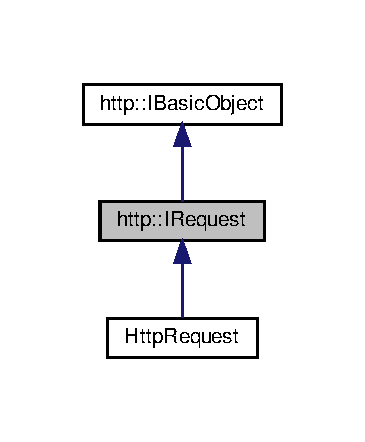
\includegraphics[width=175pt]{structhttp_1_1IRequest__inherit__graph}
\end{center}
\end{figure}


Collaboration diagram for http\+:\+:I\+Request\+:
\nopagebreak
\begin{figure}[H]
\begin{center}
\leavevmode
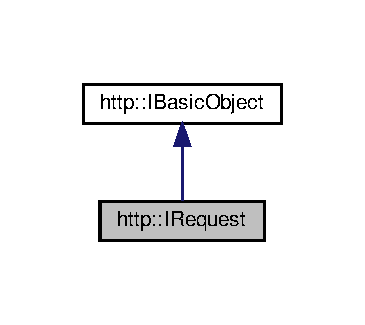
\includegraphics[width=175pt]{structhttp_1_1IRequest__coll__graph}
\end{center}
\end{figure}
\subsection*{Public Member Functions}
\begin{DoxyCompactItemize}
\item 
\mbox{\Hypertarget{structhttp_1_1IRequest_afafa06d3a8691b6faf06f2a0cc53845c}\label{structhttp_1_1IRequest_afafa06d3a8691b6faf06f2a0cc53845c}} 
virtual \hyperlink{structhttp_1_1IRequest_afafa06d3a8691b6faf06f2a0cc53845c}{$\sim$\+I\+Request} ()=default
\begin{DoxyCompactList}\small\item\em Default destructor. \end{DoxyCompactList}\item 
virtual http\+::\+Verb \hyperlink{structhttp_1_1IRequest_aef9304b69674a5c9873a33564b51d527}{verb} () const noexcept=0
\begin{DoxyCompactList}\small\item\em Returns the http verb. \end{DoxyCompactList}\item 
virtual bool \hyperlink{structhttp_1_1IRequest_abcb6f9f77b7d800677e9af3728500fa8}{verb} (http\+::\+Verb verb) noexcept=0
\begin{DoxyCompactList}\small\item\em Change the verb of the request. \end{DoxyCompactList}\item 
virtual std\+::string \hyperlink{structhttp_1_1IRequest_aa7827e21a7d25038ebc1124ae08f02de}{route} () const noexcept=0
\begin{DoxyCompactList}\small\item\em Returns the route. \end{DoxyCompactList}\item 
virtual bool \hyperlink{structhttp_1_1IRequest_a76f3dfba1e9396a0865ea133af371b80}{route} (std\+::string route) noexcept=0
\begin{DoxyCompactList}\small\item\em Change the route. \end{DoxyCompactList}\item 
virtual bool \hyperlink{structhttp_1_1IRequest_a3f2a5c8775396ac91971881d88d59c62}{query\+Parameter\+Exist} (const std\+::string \&key) const noexcept=0
\begin{DoxyCompactList}\small\item\em Checks if in the route, there are a named \textquotesingle{}key\textquotesingle{} query parameter. \end{DoxyCompactList}\item 
virtual std\+::string \hyperlink{structhttp_1_1IRequest_ae6177a18241aff420fa2e6f93195a7a7}{query\+Parameter} (const std\+::string \&key) const noexcept=0
\begin{DoxyCompactList}\small\item\em Return the query parameter \char`\"{}key\char`\"{} found in the route. \end{DoxyCompactList}\item 
virtual bool \hyperlink{structhttp_1_1IRequest_aded13d22f58bf5f622524929a52de7ef}{query\+Parameter} (std\+::string key, std\+::string value) noexcept=0
\begin{DoxyCompactList}\small\item\em Add / Update a query parameter. \end{DoxyCompactList}\item 
\mbox{\Hypertarget{structhttp_1_1IRequest_adf6b9c910c1b2ad11ac9fec2f216b16e}\label{structhttp_1_1IRequest_adf6b9c910c1b2ad11ac9fec2f216b16e}} 
virtual std\+::string \hyperlink{structhttp_1_1IRequest_adf6b9c910c1b2ad11ac9fec2f216b16e}{cookie} (const std\+::string \&name) const noexcept=0
\begin{DoxyCompactList}\small\item\em Return the value of the cookie \textquotesingle{}name\textquotesingle{} In header there are an header parameter name \textquotesingle{}Cookie\textquotesingle{} who has all cookies of the request ex\+: \char`\"{}\+Cookie\+: yummy\+\_\+cookie=choco; tasty\+\_\+cookie=strawberry\char`\"{} Return a empty string if the cookie not exist. \end{DoxyCompactList}\end{DoxyCompactItemize}


\subsection{Detailed Description}
\href{http::IRequest}{\tt http\+::\+I\+Request} is a interface that encapsulates a http request 

\subsection{Member Function Documentation}
\mbox{\Hypertarget{structhttp_1_1IRequest_ae6177a18241aff420fa2e6f93195a7a7}\label{structhttp_1_1IRequest_ae6177a18241aff420fa2e6f93195a7a7}} 
\index{http\+::\+I\+Request@{http\+::\+I\+Request}!query\+Parameter@{query\+Parameter}}
\index{query\+Parameter@{query\+Parameter}!http\+::\+I\+Request@{http\+::\+I\+Request}}
\subsubsection{\texorpdfstring{query\+Parameter()}{queryParameter()}\hspace{0.1cm}{\footnotesize\ttfamily [1/2]}}
{\footnotesize\ttfamily virtual std\+::string http\+::\+I\+Request\+::query\+Parameter (\begin{DoxyParamCaption}\item[{const std\+::string \&}]{key }\end{DoxyParamCaption}) const\hspace{0.3cm}{\ttfamily [pure virtual]}, {\ttfamily [noexcept]}}



Return the query parameter \char`\"{}key\char`\"{} found in the route. 

In \char`\"{}http\+://example.\+com/index?key=value\&test=yes\char`\"{} the query parameters are \char`\"{}key\char`\"{} and \char`\"{}test\char`\"{} for the values of \char`\"{}value\char`\"{} and \char`\"{}yes\char`\"{} Return a empty string if the parameter is not found 

Implemented in \hyperlink{classHttpRequest_a10cef7d5ff51ddc7eb5ebd2f25a0f66c}{Http\+Request}.

\mbox{\Hypertarget{structhttp_1_1IRequest_aded13d22f58bf5f622524929a52de7ef}\label{structhttp_1_1IRequest_aded13d22f58bf5f622524929a52de7ef}} 
\index{http\+::\+I\+Request@{http\+::\+I\+Request}!query\+Parameter@{query\+Parameter}}
\index{query\+Parameter@{query\+Parameter}!http\+::\+I\+Request@{http\+::\+I\+Request}}
\subsubsection{\texorpdfstring{query\+Parameter()}{queryParameter()}\hspace{0.1cm}{\footnotesize\ttfamily [2/2]}}
{\footnotesize\ttfamily virtual bool http\+::\+I\+Request\+::query\+Parameter (\begin{DoxyParamCaption}\item[{std\+::string}]{key,  }\item[{std\+::string}]{value }\end{DoxyParamCaption})\hspace{0.3cm}{\ttfamily [pure virtual]}, {\ttfamily [noexcept]}}



Add / Update a query parameter. 

In \char`\"{}http\+://example.\+com/index?key=value\&test=yes\char`\"{} the query parameters are \char`\"{}key\char`\"{} and \char`\"{}test\char`\"{} for the values of \char`\"{}value\char`\"{} and \char`\"{}yes\char`\"{} Return false if the parameter is not valid 

Implemented in \hyperlink{classHttpRequest_a09bf36e9a2c76927ee45e6c5c699c461}{Http\+Request}.

\mbox{\Hypertarget{structhttp_1_1IRequest_a3f2a5c8775396ac91971881d88d59c62}\label{structhttp_1_1IRequest_a3f2a5c8775396ac91971881d88d59c62}} 
\index{http\+::\+I\+Request@{http\+::\+I\+Request}!query\+Parameter\+Exist@{query\+Parameter\+Exist}}
\index{query\+Parameter\+Exist@{query\+Parameter\+Exist}!http\+::\+I\+Request@{http\+::\+I\+Request}}
\subsubsection{\texorpdfstring{query\+Parameter\+Exist()}{queryParameterExist()}}
{\footnotesize\ttfamily virtual bool http\+::\+I\+Request\+::query\+Parameter\+Exist (\begin{DoxyParamCaption}\item[{const std\+::string \&}]{key }\end{DoxyParamCaption}) const\hspace{0.3cm}{\ttfamily [pure virtual]}, {\ttfamily [noexcept]}}



Checks if in the route, there are a named \textquotesingle{}key\textquotesingle{} query parameter. 

In \char`\"{}http\+://example.\+com/index?key=value\&test=yes\char`\"{} the query parameters are \char`\"{}key\char`\"{} and \char`\"{}test\char`\"{} for the values of \char`\"{}value\char`\"{} and \char`\"{}yes\char`\"{} 

Implemented in \hyperlink{classHttpRequest_a81ce6a379efeba53bd3d40699462628b}{Http\+Request}.

\mbox{\Hypertarget{structhttp_1_1IRequest_aa7827e21a7d25038ebc1124ae08f02de}\label{structhttp_1_1IRequest_aa7827e21a7d25038ebc1124ae08f02de}} 
\index{http\+::\+I\+Request@{http\+::\+I\+Request}!route@{route}}
\index{route@{route}!http\+::\+I\+Request@{http\+::\+I\+Request}}
\subsubsection{\texorpdfstring{route()}{route()}\hspace{0.1cm}{\footnotesize\ttfamily [1/2]}}
{\footnotesize\ttfamily virtual std\+::string http\+::\+I\+Request\+::route (\begin{DoxyParamCaption}{ }\end{DoxyParamCaption}) const\hspace{0.3cm}{\ttfamily [pure virtual]}, {\ttfamily [noexcept]}}



Returns the route. 

In \char`\"{}http\+://example.\+com/index?key=value\&test=yes\char`\"{} returns \char`\"{}/index\char`\"{} She doesn\textquotesingle{}t returns the query parameters (\char`\"{}?key=value\&test=yes\char`\"{}) 

Implemented in \hyperlink{classHttpRequest_a313930a1717c2635ad092b7f6c7d2460}{Http\+Request}.

\mbox{\Hypertarget{structhttp_1_1IRequest_a76f3dfba1e9396a0865ea133af371b80}\label{structhttp_1_1IRequest_a76f3dfba1e9396a0865ea133af371b80}} 
\index{http\+::\+I\+Request@{http\+::\+I\+Request}!route@{route}}
\index{route@{route}!http\+::\+I\+Request@{http\+::\+I\+Request}}
\subsubsection{\texorpdfstring{route()}{route()}\hspace{0.1cm}{\footnotesize\ttfamily [2/2]}}
{\footnotesize\ttfamily virtual bool http\+::\+I\+Request\+::route (\begin{DoxyParamCaption}\item[{std\+::string}]{route }\end{DoxyParamCaption})\hspace{0.3cm}{\ttfamily [pure virtual]}, {\ttfamily [noexcept]}}



Change the route. 

In \char`\"{}http\+://example.\+com/index?key=value\&test=yes\char`\"{} returns \char`\"{}/index\char`\"{} She doesn\textquotesingle{}t returns the query parameters (\char`\"{}?key=value\&test=yes\char`\"{}) Return false if route aren\textquotesingle{}t valid 

Implemented in \hyperlink{classHttpRequest_aa71843738db71fe1f826bd30fbf5bb29}{Http\+Request}.

\mbox{\Hypertarget{structhttp_1_1IRequest_aef9304b69674a5c9873a33564b51d527}\label{structhttp_1_1IRequest_aef9304b69674a5c9873a33564b51d527}} 
\index{http\+::\+I\+Request@{http\+::\+I\+Request}!verb@{verb}}
\index{verb@{verb}!http\+::\+I\+Request@{http\+::\+I\+Request}}
\subsubsection{\texorpdfstring{verb()}{verb()}\hspace{0.1cm}{\footnotesize\ttfamily [1/2]}}
{\footnotesize\ttfamily virtual http\+::\+Verb http\+::\+I\+Request\+::verb (\begin{DoxyParamCaption}{ }\end{DoxyParamCaption}) const\hspace{0.3cm}{\ttfamily [pure virtual]}, {\ttfamily [noexcept]}}



Returns the http verb. 

The verb can be G\+ET, H\+E\+AD, P\+O\+ST, P\+UT, D\+E\+L\+E\+TE, C\+O\+N\+N\+E\+CT, O\+P\+T\+I\+O\+NS, T\+R\+A\+CE, P\+A\+T\+CH 

Implemented in \hyperlink{classHttpRequest_aded380ba96f29fb1cc6da1679a975dd8}{Http\+Request}.

\mbox{\Hypertarget{structhttp_1_1IRequest_abcb6f9f77b7d800677e9af3728500fa8}\label{structhttp_1_1IRequest_abcb6f9f77b7d800677e9af3728500fa8}} 
\index{http\+::\+I\+Request@{http\+::\+I\+Request}!verb@{verb}}
\index{verb@{verb}!http\+::\+I\+Request@{http\+::\+I\+Request}}
\subsubsection{\texorpdfstring{verb()}{verb()}\hspace{0.1cm}{\footnotesize\ttfamily [2/2]}}
{\footnotesize\ttfamily virtual bool http\+::\+I\+Request\+::verb (\begin{DoxyParamCaption}\item[{http\+::\+Verb}]{verb }\end{DoxyParamCaption})\hspace{0.3cm}{\ttfamily [pure virtual]}, {\ttfamily [noexcept]}}



Change the verb of the request. 

The verb can be G\+ET, H\+E\+AD, P\+O\+ST, P\+UT, D\+E\+L\+E\+TE, C\+O\+N\+N\+E\+CT, O\+P\+T\+I\+O\+NS, T\+R\+A\+CE, P\+A\+T\+CH Return true if there are no problems 

Implemented in \hyperlink{classHttpRequest_a243897d5dd8ba0195ce0acb6e9dd79ae}{Http\+Request}.



The documentation for this struct was generated from the following file\+:\begin{DoxyCompactItemize}
\item 
inc/\+Core/\+Http/api/I\+Request.\+hpp\end{DoxyCompactItemize}

\hypertarget{structhttp_1_1IResponse}{}\section{http\+:\+:I\+Response Struct Reference}
\label{structhttp_1_1IResponse}\index{http\+::\+I\+Response@{http\+::\+I\+Response}}


\href{http::IResponse}{\tt http\+::\+I\+Response} is a interface that encapsulates a http response  




{\ttfamily \#include $<$I\+Response.\+hpp$>$}



Inheritance diagram for http\+:\+:I\+Response\+:
\nopagebreak
\begin{figure}[H]
\begin{center}
\leavevmode
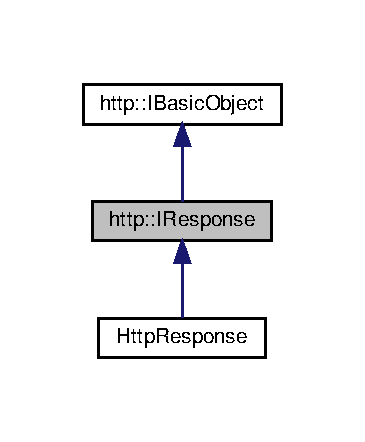
\includegraphics[width=175pt]{structhttp_1_1IResponse__inherit__graph}
\end{center}
\end{figure}


Collaboration diagram for http\+:\+:I\+Response\+:
\nopagebreak
\begin{figure}[H]
\begin{center}
\leavevmode
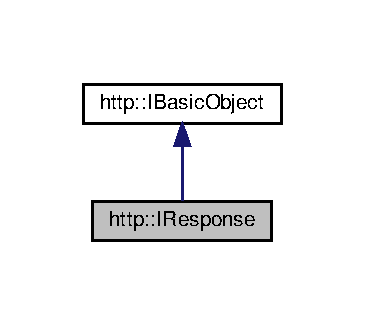
\includegraphics[width=175pt]{structhttp_1_1IResponse__coll__graph}
\end{center}
\end{figure}
\subsection*{Public Member Functions}
\begin{DoxyCompactItemize}
\item 
\mbox{\Hypertarget{structhttp_1_1IResponse_aba6a570f0288e63f38b3a8835001a94e}\label{structhttp_1_1IResponse_aba6a570f0288e63f38b3a8835001a94e}} 
virtual \hyperlink{structhttp_1_1IResponse_aba6a570f0288e63f38b3a8835001a94e}{$\sim$\+I\+Response} ()=default
\begin{DoxyCompactList}\small\item\em Default destructor. \end{DoxyCompactList}\item 
virtual int \hyperlink{structhttp_1_1IResponse_ad980a7a0b5f1de80bd1faa84706e922f}{status\+Code} () const noexcept=0
\begin{DoxyCompactList}\small\item\em Returns the status code of the response. \end{DoxyCompactList}\item 
virtual bool \hyperlink{structhttp_1_1IResponse_a7d85b2b27acb82d13cf26eb0d3801735}{status\+Code} (int status\+Code) noexcept=0
\begin{DoxyCompactList}\small\item\em Set the status code of the response. \end{DoxyCompactList}\item 
virtual std\+::string \hyperlink{structhttp_1_1IResponse_a4339fd29b105c9ea5319b2e01f27290c}{status\+Message} () const noexcept=0
\begin{DoxyCompactList}\small\item\em Returns the status message of the response. \end{DoxyCompactList}\item 
virtual bool \hyperlink{structhttp_1_1IResponse_ae2a223c2d714b456f2a064e13cafc2e2}{status\+Message} (std\+::string status\+Message) noexcept=0
\begin{DoxyCompactList}\small\item\em Set the status message of the response. \end{DoxyCompactList}\item 
\mbox{\Hypertarget{structhttp_1_1IResponse_ad682cbed4ec24a5c96979e2021794a15}\label{structhttp_1_1IResponse_ad682cbed4ec24a5c96979e2021794a15}} 
virtual bool \hyperlink{structhttp_1_1IResponse_ad682cbed4ec24a5c96979e2021794a15}{set\+Cookie} (std\+::string name, std\+::string value, Cookie\+Options options=Cookie\+Options()) noexcept=0
\begin{DoxyCompactList}\small\item\em Return the value of the cookie \textquotesingle{}name\textquotesingle{} In header there are an header parameter name \textquotesingle{}Cookie\textquotesingle{} who has all cookies of the request ex\+: \char`\"{}\+Cookie\+: yummy\+\_\+cookie=choco; tasty\+\_\+cookie=strawberry\char`\"{} He can have options like Expires, Domain, Max-\/\+Age, ... Return false if the name or the value are invalids. \end{DoxyCompactList}\end{DoxyCompactItemize}


\subsection{Detailed Description}
\href{http::IResponse}{\tt http\+::\+I\+Response} is a interface that encapsulates a http response 

\subsection{Member Function Documentation}
\mbox{\Hypertarget{structhttp_1_1IResponse_ad980a7a0b5f1de80bd1faa84706e922f}\label{structhttp_1_1IResponse_ad980a7a0b5f1de80bd1faa84706e922f}} 
\index{http\+::\+I\+Response@{http\+::\+I\+Response}!status\+Code@{status\+Code}}
\index{status\+Code@{status\+Code}!http\+::\+I\+Response@{http\+::\+I\+Response}}
\subsubsection{\texorpdfstring{status\+Code()}{statusCode()}\hspace{0.1cm}{\footnotesize\ttfamily [1/2]}}
{\footnotesize\ttfamily virtual int http\+::\+I\+Response\+::status\+Code (\begin{DoxyParamCaption}{ }\end{DoxyParamCaption}) const\hspace{0.3cm}{\ttfamily [pure virtual]}, {\ttfamily [noexcept]}}



Returns the status code of the response. 

In http response there are always status code like 200 or 404 To describe if the request is executed correctly 

Implemented in \hyperlink{classHttpResponse_a5cb28c82fc2f657808b61f0f6bb67f28}{Http\+Response}.

\mbox{\Hypertarget{structhttp_1_1IResponse_a7d85b2b27acb82d13cf26eb0d3801735}\label{structhttp_1_1IResponse_a7d85b2b27acb82d13cf26eb0d3801735}} 
\index{http\+::\+I\+Response@{http\+::\+I\+Response}!status\+Code@{status\+Code}}
\index{status\+Code@{status\+Code}!http\+::\+I\+Response@{http\+::\+I\+Response}}
\subsubsection{\texorpdfstring{status\+Code()}{statusCode()}\hspace{0.1cm}{\footnotesize\ttfamily [2/2]}}
{\footnotesize\ttfamily virtual bool http\+::\+I\+Response\+::status\+Code (\begin{DoxyParamCaption}\item[{int}]{status\+Code }\end{DoxyParamCaption})\hspace{0.3cm}{\ttfamily [pure virtual]}, {\ttfamily [noexcept]}}



Set the status code of the response. 

In http response there are always status code like \char`\"{}200\char`\"{} or \char`\"{}404\char`\"{} To describe if the request is executed correctly Return false if the status code isn\textquotesingle{}t valid 

Implemented in \hyperlink{classHttpResponse_a8a6cc8f27e81ca4d2ef4ec60450974d1}{Http\+Response}.

\mbox{\Hypertarget{structhttp_1_1IResponse_a4339fd29b105c9ea5319b2e01f27290c}\label{structhttp_1_1IResponse_a4339fd29b105c9ea5319b2e01f27290c}} 
\index{http\+::\+I\+Response@{http\+::\+I\+Response}!status\+Message@{status\+Message}}
\index{status\+Message@{status\+Message}!http\+::\+I\+Response@{http\+::\+I\+Response}}
\subsubsection{\texorpdfstring{status\+Message()}{statusMessage()}\hspace{0.1cm}{\footnotesize\ttfamily [1/2]}}
{\footnotesize\ttfamily virtual std\+::string http\+::\+I\+Response\+::status\+Message (\begin{DoxyParamCaption}{ }\end{DoxyParamCaption}) const\hspace{0.3cm}{\ttfamily [pure virtual]}, {\ttfamily [noexcept]}}



Returns the status message of the response. 

In http response there are always status message after the status code like \char`\"{}200 O\+K\char`\"{} or \char`\"{}404 Not found\char`\"{} 

Implemented in \hyperlink{classHttpResponse_a5463015a6d521c4c4da46505c0740f63}{Http\+Response}.

\mbox{\Hypertarget{structhttp_1_1IResponse_ae2a223c2d714b456f2a064e13cafc2e2}\label{structhttp_1_1IResponse_ae2a223c2d714b456f2a064e13cafc2e2}} 
\index{http\+::\+I\+Response@{http\+::\+I\+Response}!status\+Message@{status\+Message}}
\index{status\+Message@{status\+Message}!http\+::\+I\+Response@{http\+::\+I\+Response}}
\subsubsection{\texorpdfstring{status\+Message()}{statusMessage()}\hspace{0.1cm}{\footnotesize\ttfamily [2/2]}}
{\footnotesize\ttfamily virtual bool http\+::\+I\+Response\+::status\+Message (\begin{DoxyParamCaption}\item[{std\+::string}]{status\+Message }\end{DoxyParamCaption})\hspace{0.3cm}{\ttfamily [pure virtual]}, {\ttfamily [noexcept]}}



Set the status message of the response. 

In http response there are always status message after the status code like \char`\"{}200 O\+K\char`\"{} or \char`\"{}404 Not found\char`\"{} Return false if the status message isn\textquotesingle{}t valid 

Implemented in \hyperlink{classHttpResponse_ad705d5d1846c261e2ca80c24c9e1d75c}{Http\+Response}.



The documentation for this struct was generated from the following file\+:\begin{DoxyCompactItemize}
\item 
inc/\+Core/\+Http/api/I\+Response.\+hpp\end{DoxyCompactItemize}

\hypertarget{classcore_1_1ListenersControl}{}\section{core\+:\+:Listeners\+Control Class Reference}
\label{classcore_1_1ListenersControl}\index{core\+::\+Listeners\+Control@{core\+::\+Listeners\+Control}}
\subsection*{Public Member Functions}
\begin{DoxyCompactItemize}
\item 
\mbox{\Hypertarget{classcore_1_1ListenersControl_a48d93238c04cbb842dd2b34d47a3a11b}\label{classcore_1_1ListenersControl_a48d93238c04cbb842dd2b34d47a3a11b}} 
{\bfseries Listeners\+Control} (\hyperlink{classcore_1_1Configurations}{core\+::\+Configurations} \&configs)
\item 
\mbox{\Hypertarget{classcore_1_1ListenersControl_a7ec19f83caf8f35401882f7cc5a9e76a}\label{classcore_1_1ListenersControl_a7ec19f83caf8f35401882f7cc5a9e76a}} 
void {\bfseries new\+Listener} (unsigned short port)
\item 
\mbox{\Hypertarget{classcore_1_1ListenersControl_a9bd9b594fe3fcc64cacc19278de86f6c}\label{classcore_1_1ListenersControl_a9bd9b594fe3fcc64cacc19278de86f6c}} 
void {\bfseries destroy\+Listener} (unsigned short port)
\item 
\mbox{\Hypertarget{classcore_1_1ListenersControl_a6e35cf8d500dc349557f1629d1e639ad}\label{classcore_1_1ListenersControl_a6e35cf8d500dc349557f1629d1e639ad}} 
std\+::vector$<$ unsigned short $>$ {\bfseries list\+Listeners} () const
\item 
\mbox{\Hypertarget{classcore_1_1ListenersControl_a35885886edf981d3402cf4a15b9bf27b}\label{classcore_1_1ListenersControl_a35885886edf981d3402cf4a15b9bf27b}} 
\hyperlink{classcore_1_1Configurations}{core\+::\+Configurations} \& {\bfseries get\+Configurations} () const
\item 
\mbox{\Hypertarget{classcore_1_1ListenersControl_aab16c3b2cf3c0b491043d53da4ee60aa}\label{classcore_1_1ListenersControl_aab16c3b2cf3c0b491043d53da4ee60aa}} 
void {\bfseries reload} ()
\end{DoxyCompactItemize}


The documentation for this class was generated from the following files\+:\begin{DoxyCompactItemize}
\item 
inc/\+Core/\+Listeners/Listeners\+Control.\+hpp\item 
src/\+Core/\+Listeners/\hyperlink{ListenersControl_8cpp}{Listeners\+Control.\+cpp}\end{DoxyCompactItemize}

\hypertarget{classModule}{}\section{Module Class Reference}
\label{classModule}\index{Module@{Module}}


Loads module from dynamic library.  




{\ttfamily \#include $<$Module.\+hpp$>$}

\subsection*{Public Member Functions}
\begin{DoxyCompactItemize}
\item 
\mbox{\Hypertarget{classModule_a1f7e6ae9be9168b287c355b5160cea7b}\label{classModule_a1f7e6ae9be9168b287c355b5160cea7b}} 
{\bfseries Module} (const std\+::string \&path)
\item 
\mbox{\Hypertarget{classModule_a57b5394e3c8a21cdade52255ed59cefc}\label{classModule_a57b5394e3c8a21cdade52255ed59cefc}} 
\hyperlink{structmodule_1_1Api}{Api\+Type} \& {\bfseries get} ()
\item 
\mbox{\Hypertarget{classModule_a62490216d6f3d013ad51df7ff873e884}\label{classModule_a62490216d6f3d013ad51df7ff873e884}} 
const \hyperlink{structmodule_1_1Api}{Api\+Type} \& {\bfseries get} () const
\item 
\mbox{\Hypertarget{classModule_a9cc54514b4135990fccef2176f847749}\label{classModule_a9cc54514b4135990fccef2176f847749}} 
\hyperlink{structmodule_1_1Api}{Api\+Type} $\ast$ {\bfseries operator-\/$>$} ()
\item 
\mbox{\Hypertarget{classModule_a076c605faaac3b0a58690f070ea39aa8}\label{classModule_a076c605faaac3b0a58690f070ea39aa8}} 
const \hyperlink{structmodule_1_1Api}{Api\+Type} $\ast$ {\bfseries operator-\/$>$} () const
\item 
\mbox{\Hypertarget{classModule_aa8cecdcb3cff969c9255a650035c261b}\label{classModule_aa8cecdcb3cff969c9255a650035c261b}} 
const boost\+::dll\+::shared\+\_\+library \& {\bfseries get\+Library} () const
\end{DoxyCompactItemize}


\subsection{Detailed Description}
Loads module from dynamic library. 

The dynamic library M\+U\+ST provide a boost D\+LL alias {\ttfamily create\+\_\+module} to a function of signature


\begin{DoxyCode}
`ApiType` *create\_module();
\end{DoxyCode}
 

The documentation for this class was generated from the following files\+:\begin{DoxyCompactItemize}
\item 
inc/\+Core/\+Module/Module.\+hpp\item 
src/\+Core/\+Module/Module.\+cpp\end{DoxyCompactItemize}

\hypertarget{classcore_1_1config_1_1Module}{}\section{core\+:\+:config\+:\+:Module Class Reference}
\label{classcore_1_1config_1_1Module}\index{core\+::config\+::\+Module@{core\+::config\+::\+Module}}
\subsection*{Public Member Functions}
\begin{DoxyCompactItemize}
\item 
\mbox{\Hypertarget{classcore_1_1config_1_1Module_ad9499dfd277f1b8fc1053eb3198997e1}\label{classcore_1_1config_1_1Module_ad9499dfd277f1b8fc1053eb3198997e1}} 
{\bfseries Module} (const \hyperlink{classIConfigNode}{I\+Config\+Node} \&node)
\item 
\mbox{\Hypertarget{classcore_1_1config_1_1Module_ae29c6550fd5092bde84347a1271c185c}\label{classcore_1_1config_1_1Module_ae29c6550fd5092bde84347a1271c185c}} 
std\+::string {\bfseries get\+Config} (const std\+::string \&key) const
\item 
\mbox{\Hypertarget{classcore_1_1config_1_1Module_a1c7445a5221ebeaa5980e84877339775}\label{classcore_1_1config_1_1Module_a1c7445a5221ebeaa5980e84877339775}} 
const std\+::unordered\+\_\+map$<$ std\+::string, std\+::string $>$ \& {\bfseries get\+Configs} () const
\item 
\mbox{\Hypertarget{classcore_1_1config_1_1Module_af8dc4282af9a07b33fcad56931d9d6c3}\label{classcore_1_1config_1_1Module_af8dc4282af9a07b33fcad56931d9d6c3}} 
std\+::string {\bfseries get\+Name} () const
\item 
\mbox{\Hypertarget{classcore_1_1config_1_1Module_a352e825070ab2e7566de1c1cc97fa93a}\label{classcore_1_1config_1_1Module_a352e825070ab2e7566de1c1cc97fa93a}} 
std\+::vector$<$ std\+::string $>$ {\bfseries get\+Configs\+Name} () const
\item 
\mbox{\Hypertarget{classcore_1_1config_1_1Module_a304e4e49730ee44150843b1823bcb6ef}\label{classcore_1_1config_1_1Module_a304e4e49730ee44150843b1823bcb6ef}} 
bool {\bfseries has\+Config} (const std\+::string \&key) const
\end{DoxyCompactItemize}


The documentation for this class was generated from the following files\+:\begin{DoxyCompactItemize}
\item 
inc/\+Core/\+Configs/\hyperlink{Modules_8hpp}{Modules.\+hpp}\item 
src/\+Core/\+Configs/Module.\+cpp\end{DoxyCompactItemize}

\hypertarget{classcore_1_1config_1_1ModulesContainer}{}\section{core\+:\+:config\+:\+:Modules\+Container Class Reference}
\label{classcore_1_1config_1_1ModulesContainer}\index{core\+::config\+::\+Modules\+Container@{core\+::config\+::\+Modules\+Container}}


Inheritance diagram for core\+:\+:config\+:\+:Modules\+Container\+:
\nopagebreak
\begin{figure}[H]
\begin{center}
\leavevmode
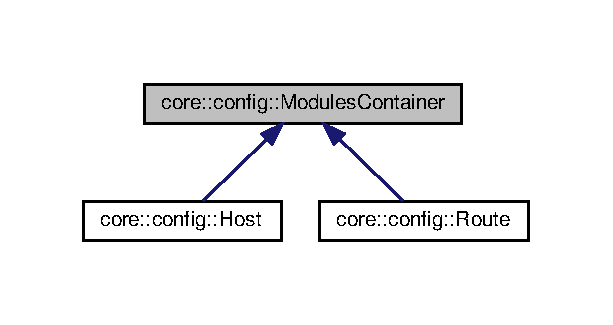
\includegraphics[width=294pt]{classcore_1_1config_1_1ModulesContainer__inherit__graph}
\end{center}
\end{figure}
\subsection*{Public Member Functions}
\begin{DoxyCompactItemize}
\item 
\mbox{\Hypertarget{classcore_1_1config_1_1ModulesContainer_a7c1e7b912e1310059e7bfe3a48cb0688}\label{classcore_1_1config_1_1ModulesContainer_a7c1e7b912e1310059e7bfe3a48cb0688}} 
std\+::vector$<$ std\+::string $>$ {\bfseries get\+Modules\+Name} () const
\item 
\mbox{\Hypertarget{classcore_1_1config_1_1ModulesContainer_a9a12b9494161665e47e96124f1833178}\label{classcore_1_1config_1_1ModulesContainer_a9a12b9494161665e47e96124f1833178}} 
const std\+::unordered\+\_\+map$<$ std\+::string, \hyperlink{classcore_1_1config_1_1Module}{core\+::config\+::\+Module} $>$ \& {\bfseries get\+Modules} () const
\item 
\mbox{\Hypertarget{classcore_1_1config_1_1ModulesContainer_a8be58c3b8ada51dc2834e1e142746686}\label{classcore_1_1config_1_1ModulesContainer_a8be58c3b8ada51dc2834e1e142746686}} 
\hyperlink{classcore_1_1config_1_1Module}{core\+::config\+::\+Module} {\bfseries get\+Module} (const std\+::string \&name) const
\item 
\mbox{\Hypertarget{classcore_1_1config_1_1ModulesContainer_abc911e006a70687a07fa79d755045dea}\label{classcore_1_1config_1_1ModulesContainer_abc911e006a70687a07fa79d755045dea}} 
bool {\bfseries has\+Module} (const std\+::string \&name) const
\end{DoxyCompactItemize}
\subsection*{Protected Member Functions}
\begin{DoxyCompactItemize}
\item 
\mbox{\Hypertarget{classcore_1_1config_1_1ModulesContainer_ab6ada155227703fdd81f22c2047ffdc2}\label{classcore_1_1config_1_1ModulesContainer_ab6ada155227703fdd81f22c2047ffdc2}} 
void {\bfseries add\+Module} (const \hyperlink{classIConfigNode}{I\+Config\+Node} \&config)
\end{DoxyCompactItemize}


The documentation for this class was generated from the following files\+:\begin{DoxyCompactItemize}
\item 
inc/\+Core/\+Configs/\hyperlink{ModulesContainer_8hpp}{Modules\+Container.\+hpp}\item 
src/\+Core/\+Configs/\hyperlink{ModulesContainer_8cpp}{Modules\+Container.\+cpp}\end{DoxyCompactItemize}

\hypertarget{classnet_1_1NetworkManager}{}\section{net\+:\+:Network\+Manager Class Reference}
\label{classnet_1_1NetworkManager}\index{net\+::\+Network\+Manager@{net\+::\+Network\+Manager}}
\subsection*{Public Member Functions}
\begin{DoxyCompactItemize}
\item 
\mbox{\Hypertarget{classnet_1_1NetworkManager_ae958994e668d631672db8d6b83dd2076}\label{classnet_1_1NetworkManager_ae958994e668d631672db8d6b83dd2076}} 
{\bfseries Network\+Manager} (const \hyperlink{classcore_1_1config_1_1Host}{core\+::config\+::\+Host} \&configs)
\item 
\mbox{\Hypertarget{classnet_1_1NetworkManager_aa33a78312f6596a6d148b63cd1e8ffd6}\label{classnet_1_1NetworkManager_aa33a78312f6596a6d148b63cd1e8ffd6}} 
void {\bfseries new\+Client} (boost\+::shared\+\_\+ptr$<$ \hyperlink{structnet_1_1IClient}{net\+::\+I\+Client} $>$ client)
\item 
\mbox{\Hypertarget{classnet_1_1NetworkManager_a4cd3c13ec5e4598277e7e26a943a00db}\label{classnet_1_1NetworkManager_a4cd3c13ec5e4598277e7e26a943a00db}} 
void {\bfseries remove\+Client} (boost\+::shared\+\_\+ptr$<$ \hyperlink{structnet_1_1IClient}{net\+::\+I\+Client} $>$ client)
\item 
\mbox{\Hypertarget{classnet_1_1NetworkManager_afa7e0c3ab9414749c09a16e73fd1d61c}\label{classnet_1_1NetworkManager_afa7e0c3ab9414749c09a16e73fd1d61c}} 
void {\bfseries recv\+Data} (boost\+::shared\+\_\+ptr$<$ \hyperlink{structnet_1_1IClient}{net\+::\+I\+Client} $>$ client, std\+::string \&data)
\end{DoxyCompactItemize}


The documentation for this class was generated from the following files\+:\begin{DoxyCompactItemize}
\item 
inc/\+Network/\hyperlink{NetworkManager_8hpp}{Network\+Manager.\+hpp}\item 
src/\+Network/\hyperlink{NetworkManager_8cpp}{Network\+Manager.\+cpp}\end{DoxyCompactItemize}

\hypertarget{classmodule_1_1Php}{}\section{module\+:\+:Php Class Reference}
\label{classmodule_1_1Php}\index{module\+::\+Php@{module\+::\+Php}}


Inheritance diagram for module\+:\+:Php\+:
\nopagebreak
\begin{figure}[H]
\begin{center}
\leavevmode
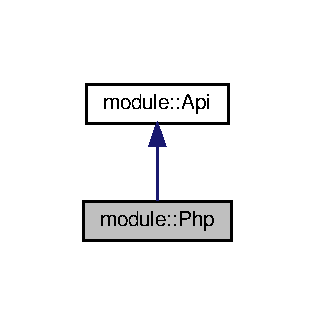
\includegraphics[width=151pt]{classmodule_1_1Php__inherit__graph}
\end{center}
\end{figure}


Collaboration diagram for module\+:\+:Php\+:
\nopagebreak
\begin{figure}[H]
\begin{center}
\leavevmode
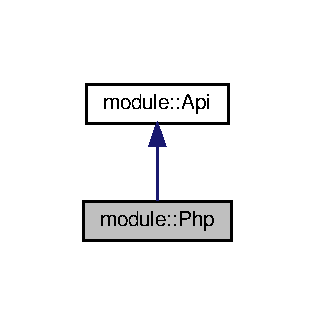
\includegraphics[width=151pt]{classmodule_1_1Php__coll__graph}
\end{center}
\end{figure}
\subsection*{Public Member Functions}
\begin{DoxyCompactItemize}
\item 
\mbox{\Hypertarget{classmodule_1_1Php_a0c36f6f31d9bc9459c19cc65781c03e3}\label{classmodule_1_1Php_a0c36f6f31d9bc9459c19cc65781c03e3}} 
std\+::string \hyperlink{classmodule_1_1Php_a0c36f6f31d9bc9459c19cc65781c03e3}{name} () const noexcept
\begin{DoxyCompactList}\small\item\em Returns the module name. \end{DoxyCompactList}\item 
bool \hyperlink{classmodule_1_1Php_adc03ae040e0a938640bd4ba9a6eb2d3c}{new\+Connection} (const \hyperlink{structnet_1_1IClient}{net\+::\+I\+Client} \&client) noexcept
\begin{DoxyCompactList}\small\item\em When a new client connects to the http server. \end{DoxyCompactList}\item 
bool \hyperlink{classmodule_1_1Php_af828a98b73d3da6a53a64d4b3b3927c4}{disconnection} (const \hyperlink{structnet_1_1IClient}{net\+::\+I\+Client} \&client) noexcept
\begin{DoxyCompactList}\small\item\em When a client disconnects. \end{DoxyCompactList}\item 
\mbox{\Hypertarget{classmodule_1_1Php_a3a71c84751d3333ad538826d7a485bac}\label{classmodule_1_1Php_a3a71c84751d3333ad538826d7a485bac}} 
bool \hyperlink{classmodule_1_1Php_a3a71c84751d3333ad538826d7a485bac}{set\+Configurations} (Configs configs) noexcept
\begin{DoxyCompactList}\small\item\em Set the Global configs of the module. \end{DoxyCompactList}\item 
bool \hyperlink{classmodule_1_1Php_a553dd60d283baf309a9ba8ddb87681b8}{after\+Receive} (const \hyperlink{structnet_1_1IClient}{net\+::\+I\+Client} \&client, std\+::string \&buffer) noexcept
\begin{DoxyCompactList}\small\item\em Just before the deserialization of the packet. \end{DoxyCompactList}\item 
bool \hyperlink{classmodule_1_1Php_ae3f23ea75718c51e0427fa2d13ab9755}{after\+Unpacked} (const \hyperlink{structnet_1_1IClient}{net\+::\+I\+Client} \&client, \hyperlink{structhttp_1_1IRequest}{http\+::\+I\+Request} \&request) noexcept
\begin{DoxyCompactList}\small\item\em Call before the main behavior of the module. \end{DoxyCompactList}\item 
bool \hyperlink{classmodule_1_1Php_aa73bfe086a0015a892f7d5687639aafb}{execute} (const \hyperlink{structnet_1_1IClient}{net\+::\+I\+Client} \&client, \hyperlink{structhttp_1_1IRequest}{http\+::\+I\+Request} \&request, \hyperlink{structhttp_1_1IResponse}{http\+::\+I\+Response} \&response) noexcept
\begin{DoxyCompactList}\small\item\em This is the main behavior of the module. \end{DoxyCompactList}\item 
bool \hyperlink{classmodule_1_1Php_a71b22ae01eedfd3406d01907cd7dc3d9}{before\+Packed} (const \hyperlink{structnet_1_1IClient}{net\+::\+I\+Client} \&client, \hyperlink{structhttp_1_1IResponse}{http\+::\+I\+Response} \&response) noexcept
\begin{DoxyCompactList}\small\item\em Just before the serialization of the response. \end{DoxyCompactList}\item 
bool \hyperlink{classmodule_1_1Php_a9ba9768f149e9dbf3094d5cdb4967fc3}{before\+Send} (const \hyperlink{structnet_1_1IClient}{net\+::\+I\+Client} \&client, std\+::string \&buffer) noexcept
\begin{DoxyCompactList}\small\item\em Just before packet delivery. \end{DoxyCompactList}\end{DoxyCompactItemize}


\subsection{Member Function Documentation}
\mbox{\Hypertarget{classmodule_1_1Php_a553dd60d283baf309a9ba8ddb87681b8}\label{classmodule_1_1Php_a553dd60d283baf309a9ba8ddb87681b8}} 
\index{module\+::\+Php@{module\+::\+Php}!after\+Receive@{after\+Receive}}
\index{after\+Receive@{after\+Receive}!module\+::\+Php@{module\+::\+Php}}
\subsubsection{\texorpdfstring{after\+Receive()}{afterReceive()}}
{\footnotesize\ttfamily bool module\+::\+Php\+::after\+Receive (\begin{DoxyParamCaption}\item[{const \hyperlink{structnet_1_1IClient}{net\+::\+I\+Client} \&}]{client,  }\item[{std\+::string \&}]{buffer }\end{DoxyParamCaption})\hspace{0.3cm}{\ttfamily [virtual]}, {\ttfamily [noexcept]}}



Just before the deserialization of the packet. 

It can be useful to decrypt an tls packet 

Implements \hyperlink{structmodule_1_1Api_ad8b56820e4f53bf65d34447184edef20}{module\+::\+Api}.

\mbox{\Hypertarget{classmodule_1_1Php_ae3f23ea75718c51e0427fa2d13ab9755}\label{classmodule_1_1Php_ae3f23ea75718c51e0427fa2d13ab9755}} 
\index{module\+::\+Php@{module\+::\+Php}!after\+Unpacked@{after\+Unpacked}}
\index{after\+Unpacked@{after\+Unpacked}!module\+::\+Php@{module\+::\+Php}}
\subsubsection{\texorpdfstring{after\+Unpacked()}{afterUnpacked()}}
{\footnotesize\ttfamily bool module\+::\+Php\+::after\+Unpacked (\begin{DoxyParamCaption}\item[{const \hyperlink{structnet_1_1IClient}{net\+::\+I\+Client} \&}]{client,  }\item[{\hyperlink{structhttp_1_1IRequest}{http\+::\+I\+Request} \&}]{request }\end{DoxyParamCaption})\hspace{0.3cm}{\ttfamily [virtual]}, {\ttfamily [noexcept]}}



Call before the main behavior of the module. 

It can be useful to decompresses a http body (gzip, ...) 

Implements \hyperlink{structmodule_1_1Api_a291297e6d233e69b82c976e085f7c237}{module\+::\+Api}.

\mbox{\Hypertarget{classmodule_1_1Php_a71b22ae01eedfd3406d01907cd7dc3d9}\label{classmodule_1_1Php_a71b22ae01eedfd3406d01907cd7dc3d9}} 
\index{module\+::\+Php@{module\+::\+Php}!before\+Packed@{before\+Packed}}
\index{before\+Packed@{before\+Packed}!module\+::\+Php@{module\+::\+Php}}
\subsubsection{\texorpdfstring{before\+Packed()}{beforePacked()}}
{\footnotesize\ttfamily bool module\+::\+Php\+::before\+Packed (\begin{DoxyParamCaption}\item[{const \hyperlink{structnet_1_1IClient}{net\+::\+I\+Client} \&}]{client,  }\item[{\hyperlink{structhttp_1_1IResponse}{http\+::\+I\+Response} \&}]{response }\end{DoxyParamCaption})\hspace{0.3cm}{\ttfamily [virtual]}, {\ttfamily [noexcept]}}



Just before the serialization of the response. 

Useful if we need to add something in the packet or to compress it 

Implements \hyperlink{structmodule_1_1Api_a5293babe6b28a397b7a11f32da0a6f51}{module\+::\+Api}.

\mbox{\Hypertarget{classmodule_1_1Php_a9ba9768f149e9dbf3094d5cdb4967fc3}\label{classmodule_1_1Php_a9ba9768f149e9dbf3094d5cdb4967fc3}} 
\index{module\+::\+Php@{module\+::\+Php}!before\+Send@{before\+Send}}
\index{before\+Send@{before\+Send}!module\+::\+Php@{module\+::\+Php}}
\subsubsection{\texorpdfstring{before\+Send()}{beforeSend()}}
{\footnotesize\ttfamily bool module\+::\+Php\+::before\+Send (\begin{DoxyParamCaption}\item[{const \hyperlink{structnet_1_1IClient}{net\+::\+I\+Client} \&}]{client,  }\item[{std\+::string \&}]{buffer }\end{DoxyParamCaption})\hspace{0.3cm}{\ttfamily [virtual]}, {\ttfamily [noexcept]}}



Just before packet delivery. 

Useful if we need to add something in the packet or to encrypt 

Implements \hyperlink{structmodule_1_1Api_a71d1ada8bc5fc81fd71607315dd86185}{module\+::\+Api}.

\mbox{\Hypertarget{classmodule_1_1Php_af828a98b73d3da6a53a64d4b3b3927c4}\label{classmodule_1_1Php_af828a98b73d3da6a53a64d4b3b3927c4}} 
\index{module\+::\+Php@{module\+::\+Php}!disconnection@{disconnection}}
\index{disconnection@{disconnection}!module\+::\+Php@{module\+::\+Php}}
\subsubsection{\texorpdfstring{disconnection()}{disconnection()}}
{\footnotesize\ttfamily bool module\+::\+Php\+::disconnection (\begin{DoxyParamCaption}\item[{const \hyperlink{structnet_1_1IClient}{net\+::\+I\+Client} \&}]{client }\end{DoxyParamCaption})\hspace{0.3cm}{\ttfamily [virtual]}, {\ttfamily [noexcept]}}



When a client disconnects. 

To inform the module of the client\textquotesingle{}s disconnection 

Implements \hyperlink{structmodule_1_1Api_a8aa98bd4094fb13916e100509a948763}{module\+::\+Api}.

\mbox{\Hypertarget{classmodule_1_1Php_aa73bfe086a0015a892f7d5687639aafb}\label{classmodule_1_1Php_aa73bfe086a0015a892f7d5687639aafb}} 
\index{module\+::\+Php@{module\+::\+Php}!execute@{execute}}
\index{execute@{execute}!module\+::\+Php@{module\+::\+Php}}
\subsubsection{\texorpdfstring{execute()}{execute()}}
{\footnotesize\ttfamily bool module\+::\+Php\+::execute (\begin{DoxyParamCaption}\item[{const \hyperlink{structnet_1_1IClient}{net\+::\+I\+Client} \&}]{client,  }\item[{\hyperlink{structhttp_1_1IRequest}{http\+::\+I\+Request} \&}]{request,  }\item[{\hyperlink{structhttp_1_1IResponse}{http\+::\+I\+Response} \&}]{response }\end{DoxyParamCaption})\hspace{0.3cm}{\ttfamily [virtual]}, {\ttfamily [noexcept]}}



This is the main behavior of the module. 

Reaction to the client\textquotesingle{}s request 

Implements \hyperlink{structmodule_1_1Api_afd1f5243a90811d06d96f725490bcba6}{module\+::\+Api}.

\mbox{\Hypertarget{classmodule_1_1Php_adc03ae040e0a938640bd4ba9a6eb2d3c}\label{classmodule_1_1Php_adc03ae040e0a938640bd4ba9a6eb2d3c}} 
\index{module\+::\+Php@{module\+::\+Php}!new\+Connection@{new\+Connection}}
\index{new\+Connection@{new\+Connection}!module\+::\+Php@{module\+::\+Php}}
\subsubsection{\texorpdfstring{new\+Connection()}{newConnection()}}
{\footnotesize\ttfamily bool module\+::\+Php\+::new\+Connection (\begin{DoxyParamCaption}\item[{const \hyperlink{structnet_1_1IClient}{net\+::\+I\+Client} \&}]{client }\end{DoxyParamCaption})\hspace{0.3cm}{\ttfamily [virtual]}, {\ttfamily [noexcept]}}



When a new client connects to the http server. 

It can be useful to store the id of the client to recognize him after 

Implements \hyperlink{structmodule_1_1Api_aa83ddc92765200dd65f915498175c2be}{module\+::\+Api}.



The documentation for this class was generated from the following files\+:\begin{DoxyCompactItemize}
\item 
modules/\+Php/\hyperlink{Php_8hpp}{Php.\+hpp}\item 
modules/\+Php/\hyperlink{Php_8cpp}{Php.\+cpp}\end{DoxyCompactItemize}

\hypertarget{classmodule_1_1Proxy}{}\section{module\+:\+:Proxy Class Reference}
\label{classmodule_1_1Proxy}\index{module\+::\+Proxy@{module\+::\+Proxy}}


Inheritance diagram for module\+:\+:Proxy\+:
\nopagebreak
\begin{figure}[H]
\begin{center}
\leavevmode
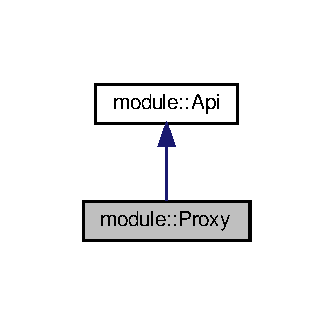
\includegraphics[width=160pt]{classmodule_1_1Proxy__inherit__graph}
\end{center}
\end{figure}


Collaboration diagram for module\+:\+:Proxy\+:
\nopagebreak
\begin{figure}[H]
\begin{center}
\leavevmode
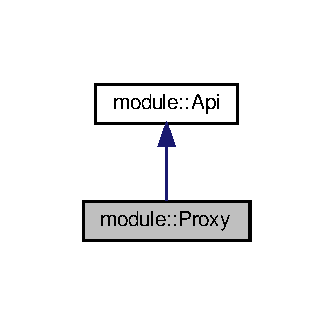
\includegraphics[width=160pt]{classmodule_1_1Proxy__coll__graph}
\end{center}
\end{figure}
\subsection*{Public Member Functions}
\begin{DoxyCompactItemize}
\item 
\mbox{\Hypertarget{classmodule_1_1Proxy_a31e224e72c2ff7c06191d4797089094d}\label{classmodule_1_1Proxy_a31e224e72c2ff7c06191d4797089094d}} 
std\+::string \hyperlink{classmodule_1_1Proxy_a31e224e72c2ff7c06191d4797089094d}{name} () const noexcept
\begin{DoxyCompactList}\small\item\em Returns the module name. \end{DoxyCompactList}\item 
bool \hyperlink{classmodule_1_1Proxy_a92e33605f1164599922fa64d936f5b77}{new\+Connection} (const \hyperlink{structnet_1_1IClient}{net\+::\+I\+Client} \&client) noexcept
\begin{DoxyCompactList}\small\item\em When a new client connects to the http server. \end{DoxyCompactList}\item 
bool \hyperlink{classmodule_1_1Proxy_aa80f5772c7c4613060f4cf49f1fc00e4}{disconnection} (const \hyperlink{structnet_1_1IClient}{net\+::\+I\+Client} \&client) noexcept
\begin{DoxyCompactList}\small\item\em When a client disconnects. \end{DoxyCompactList}\item 
\mbox{\Hypertarget{classmodule_1_1Proxy_a82ac1eab4bc1b25c0cef3a1fc4839649}\label{classmodule_1_1Proxy_a82ac1eab4bc1b25c0cef3a1fc4839649}} 
bool \hyperlink{classmodule_1_1Proxy_a82ac1eab4bc1b25c0cef3a1fc4839649}{set\+Configurations} (Configs configs) noexcept
\begin{DoxyCompactList}\small\item\em Set the Global configs of the module. \end{DoxyCompactList}\item 
bool \hyperlink{classmodule_1_1Proxy_a0dbbd27ea29602830d770c5c550b1ee4}{after\+Receive} (const \hyperlink{structnet_1_1IClient}{net\+::\+I\+Client} \&client, std\+::string \&buffer) noexcept
\begin{DoxyCompactList}\small\item\em Just before the deserialization of the packet. \end{DoxyCompactList}\item 
bool \hyperlink{classmodule_1_1Proxy_a16524232b12bd03353c79bcda4bd8d15}{after\+Unpacked} (const \hyperlink{structnet_1_1IClient}{net\+::\+I\+Client} \&client, \hyperlink{structhttp_1_1IRequest}{http\+::\+I\+Request} \&request) noexcept
\begin{DoxyCompactList}\small\item\em Call before the main behavior of the module. \end{DoxyCompactList}\item 
bool \hyperlink{classmodule_1_1Proxy_a7a210c144da81f379a7ca6b7ef7914c8}{execute} (const \hyperlink{structnet_1_1IClient}{net\+::\+I\+Client} \&client, \hyperlink{structhttp_1_1IRequest}{http\+::\+I\+Request} \&request, \hyperlink{structhttp_1_1IResponse}{http\+::\+I\+Response} \&response) noexcept
\begin{DoxyCompactList}\small\item\em This is the main behavior of the module. \end{DoxyCompactList}\item 
bool \hyperlink{classmodule_1_1Proxy_a3b88487ecaaa856f319d78f2aa6358c1}{before\+Packed} (const \hyperlink{structnet_1_1IClient}{net\+::\+I\+Client} \&client, \hyperlink{structhttp_1_1IResponse}{http\+::\+I\+Response} \&response) noexcept
\begin{DoxyCompactList}\small\item\em Just before the serialization of the response. \end{DoxyCompactList}\item 
bool \hyperlink{classmodule_1_1Proxy_a314d53ca09edbb7f2595cefb5c55771e}{before\+Send} (const \hyperlink{structnet_1_1IClient}{net\+::\+I\+Client} \&client, std\+::string \&buffer) noexcept
\begin{DoxyCompactList}\small\item\em Just before packet delivery. \end{DoxyCompactList}\end{DoxyCompactItemize}


\subsection{Member Function Documentation}
\mbox{\Hypertarget{classmodule_1_1Proxy_a0dbbd27ea29602830d770c5c550b1ee4}\label{classmodule_1_1Proxy_a0dbbd27ea29602830d770c5c550b1ee4}} 
\index{module\+::\+Proxy@{module\+::\+Proxy}!after\+Receive@{after\+Receive}}
\index{after\+Receive@{after\+Receive}!module\+::\+Proxy@{module\+::\+Proxy}}
\subsubsection{\texorpdfstring{after\+Receive()}{afterReceive()}}
{\footnotesize\ttfamily bool module\+::\+Proxy\+::after\+Receive (\begin{DoxyParamCaption}\item[{const \hyperlink{structnet_1_1IClient}{net\+::\+I\+Client} \&}]{client,  }\item[{std\+::string \&}]{buffer }\end{DoxyParamCaption})\hspace{0.3cm}{\ttfamily [virtual]}, {\ttfamily [noexcept]}}



Just before the deserialization of the packet. 

It can be useful to decrypt an tls packet 

Implements \hyperlink{structmodule_1_1Api_ad8b56820e4f53bf65d34447184edef20}{module\+::\+Api}.

\mbox{\Hypertarget{classmodule_1_1Proxy_a16524232b12bd03353c79bcda4bd8d15}\label{classmodule_1_1Proxy_a16524232b12bd03353c79bcda4bd8d15}} 
\index{module\+::\+Proxy@{module\+::\+Proxy}!after\+Unpacked@{after\+Unpacked}}
\index{after\+Unpacked@{after\+Unpacked}!module\+::\+Proxy@{module\+::\+Proxy}}
\subsubsection{\texorpdfstring{after\+Unpacked()}{afterUnpacked()}}
{\footnotesize\ttfamily bool module\+::\+Proxy\+::after\+Unpacked (\begin{DoxyParamCaption}\item[{const \hyperlink{structnet_1_1IClient}{net\+::\+I\+Client} \&}]{client,  }\item[{\hyperlink{structhttp_1_1IRequest}{http\+::\+I\+Request} \&}]{request }\end{DoxyParamCaption})\hspace{0.3cm}{\ttfamily [virtual]}, {\ttfamily [noexcept]}}



Call before the main behavior of the module. 

It can be useful to decompresses a http body (gzip, ...) 

Implements \hyperlink{structmodule_1_1Api_a291297e6d233e69b82c976e085f7c237}{module\+::\+Api}.

\mbox{\Hypertarget{classmodule_1_1Proxy_a3b88487ecaaa856f319d78f2aa6358c1}\label{classmodule_1_1Proxy_a3b88487ecaaa856f319d78f2aa6358c1}} 
\index{module\+::\+Proxy@{module\+::\+Proxy}!before\+Packed@{before\+Packed}}
\index{before\+Packed@{before\+Packed}!module\+::\+Proxy@{module\+::\+Proxy}}
\subsubsection{\texorpdfstring{before\+Packed()}{beforePacked()}}
{\footnotesize\ttfamily bool module\+::\+Proxy\+::before\+Packed (\begin{DoxyParamCaption}\item[{const \hyperlink{structnet_1_1IClient}{net\+::\+I\+Client} \&}]{client,  }\item[{\hyperlink{structhttp_1_1IResponse}{http\+::\+I\+Response} \&}]{response }\end{DoxyParamCaption})\hspace{0.3cm}{\ttfamily [virtual]}, {\ttfamily [noexcept]}}



Just before the serialization of the response. 

Useful if we need to add something in the packet or to compress it 

Implements \hyperlink{structmodule_1_1Api_a5293babe6b28a397b7a11f32da0a6f51}{module\+::\+Api}.

\mbox{\Hypertarget{classmodule_1_1Proxy_a314d53ca09edbb7f2595cefb5c55771e}\label{classmodule_1_1Proxy_a314d53ca09edbb7f2595cefb5c55771e}} 
\index{module\+::\+Proxy@{module\+::\+Proxy}!before\+Send@{before\+Send}}
\index{before\+Send@{before\+Send}!module\+::\+Proxy@{module\+::\+Proxy}}
\subsubsection{\texorpdfstring{before\+Send()}{beforeSend()}}
{\footnotesize\ttfamily bool module\+::\+Proxy\+::before\+Send (\begin{DoxyParamCaption}\item[{const \hyperlink{structnet_1_1IClient}{net\+::\+I\+Client} \&}]{client,  }\item[{std\+::string \&}]{buffer }\end{DoxyParamCaption})\hspace{0.3cm}{\ttfamily [virtual]}, {\ttfamily [noexcept]}}



Just before packet delivery. 

Useful if we need to add something in the packet or to encrypt 

Implements \hyperlink{structmodule_1_1Api_a71d1ada8bc5fc81fd71607315dd86185}{module\+::\+Api}.

\mbox{\Hypertarget{classmodule_1_1Proxy_aa80f5772c7c4613060f4cf49f1fc00e4}\label{classmodule_1_1Proxy_aa80f5772c7c4613060f4cf49f1fc00e4}} 
\index{module\+::\+Proxy@{module\+::\+Proxy}!disconnection@{disconnection}}
\index{disconnection@{disconnection}!module\+::\+Proxy@{module\+::\+Proxy}}
\subsubsection{\texorpdfstring{disconnection()}{disconnection()}}
{\footnotesize\ttfamily bool module\+::\+Proxy\+::disconnection (\begin{DoxyParamCaption}\item[{const \hyperlink{structnet_1_1IClient}{net\+::\+I\+Client} \&}]{client }\end{DoxyParamCaption})\hspace{0.3cm}{\ttfamily [virtual]}, {\ttfamily [noexcept]}}



When a client disconnects. 

To inform the module of the client\textquotesingle{}s disconnection 

Implements \hyperlink{structmodule_1_1Api_a8aa98bd4094fb13916e100509a948763}{module\+::\+Api}.

\mbox{\Hypertarget{classmodule_1_1Proxy_a7a210c144da81f379a7ca6b7ef7914c8}\label{classmodule_1_1Proxy_a7a210c144da81f379a7ca6b7ef7914c8}} 
\index{module\+::\+Proxy@{module\+::\+Proxy}!execute@{execute}}
\index{execute@{execute}!module\+::\+Proxy@{module\+::\+Proxy}}
\subsubsection{\texorpdfstring{execute()}{execute()}}
{\footnotesize\ttfamily bool module\+::\+Proxy\+::execute (\begin{DoxyParamCaption}\item[{const \hyperlink{structnet_1_1IClient}{net\+::\+I\+Client} \&}]{client,  }\item[{\hyperlink{structhttp_1_1IRequest}{http\+::\+I\+Request} \&}]{request,  }\item[{\hyperlink{structhttp_1_1IResponse}{http\+::\+I\+Response} \&}]{response }\end{DoxyParamCaption})\hspace{0.3cm}{\ttfamily [virtual]}, {\ttfamily [noexcept]}}



This is the main behavior of the module. 

Reaction to the client\textquotesingle{}s request 

Implements \hyperlink{structmodule_1_1Api_afd1f5243a90811d06d96f725490bcba6}{module\+::\+Api}.

\mbox{\Hypertarget{classmodule_1_1Proxy_a92e33605f1164599922fa64d936f5b77}\label{classmodule_1_1Proxy_a92e33605f1164599922fa64d936f5b77}} 
\index{module\+::\+Proxy@{module\+::\+Proxy}!new\+Connection@{new\+Connection}}
\index{new\+Connection@{new\+Connection}!module\+::\+Proxy@{module\+::\+Proxy}}
\subsubsection{\texorpdfstring{new\+Connection()}{newConnection()}}
{\footnotesize\ttfamily bool module\+::\+Proxy\+::new\+Connection (\begin{DoxyParamCaption}\item[{const \hyperlink{structnet_1_1IClient}{net\+::\+I\+Client} \&}]{client }\end{DoxyParamCaption})\hspace{0.3cm}{\ttfamily [virtual]}, {\ttfamily [noexcept]}}



When a new client connects to the http server. 

It can be useful to store the id of the client to recognize him after 

Implements \hyperlink{structmodule_1_1Api_aa83ddc92765200dd65f915498175c2be}{module\+::\+Api}.



The documentation for this class was generated from the following files\+:\begin{DoxyCompactItemize}
\item 
modules/\+Proxy/\hyperlink{Proxy_8hpp}{Proxy.\+hpp}\item 
modules/\+Proxy/\hyperlink{Proxy_8cpp}{Proxy.\+cpp}\end{DoxyCompactItemize}

\hypertarget{classRedirector}{}\section{Redirector Class Reference}
\label{classRedirector}\index{Redirector@{Redirector}}


Redirect ostream to get their content.  




{\ttfamily \#include $<$Redirector.\+hpp$>$}

\subsection*{Public Member Functions}
\begin{DoxyCompactItemize}
\item 
\mbox{\Hypertarget{classRedirector_a6137320fddd205c1d5b115ebf795c4e4}\label{classRedirector_a6137320fddd205c1d5b115ebf795c4e4}} 
{\bfseries Redirector} (std\+::ostream \&stream)
\item 
\mbox{\Hypertarget{classRedirector_afdb8037990faef1a1893af8a9a7a36b6}\label{classRedirector_afdb8037990faef1a1893af8a9a7a36b6}} 
std\+::string {\bfseries get\+Content} ()
\end{DoxyCompactItemize}


\subsection{Detailed Description}
Redirect ostream to get their content. 

The documentation for this class was generated from the following file\+:\begin{DoxyCompactItemize}
\item 
tests/\hyperlink{Redirector_8hpp}{Redirector.\+hpp}\end{DoxyCompactItemize}

\hypertarget{classcore_1_1config_1_1Route}{}\section{core\+:\+:config\+:\+:Route Class Reference}
\label{classcore_1_1config_1_1Route}\index{core\+::config\+::\+Route@{core\+::config\+::\+Route}}


Inheritance diagram for core\+:\+:config\+:\+:Route\+:
\nopagebreak
\begin{figure}[H]
\begin{center}
\leavevmode
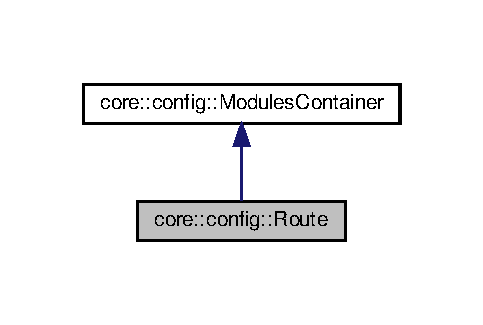
\includegraphics[width=232pt]{classcore_1_1config_1_1Route__inherit__graph}
\end{center}
\end{figure}


Collaboration diagram for core\+:\+:config\+:\+:Route\+:
\nopagebreak
\begin{figure}[H]
\begin{center}
\leavevmode
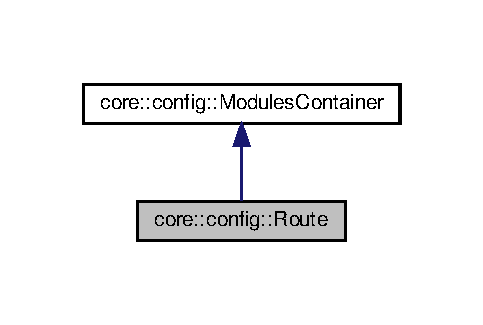
\includegraphics[width=232pt]{classcore_1_1config_1_1Route__coll__graph}
\end{center}
\end{figure}
\subsection*{Public Member Functions}
\begin{DoxyCompactItemize}
\item 
\hyperlink{classcore_1_1config_1_1Route_ae4cd245ca558e741202ebab6fa13e4e0}{Route} (const \hyperlink{classIConfigNode}{I\+Config\+Node} \&node)
\item 
\mbox{\Hypertarget{classcore_1_1config_1_1Route_a12fe2266630535ccac80d518eda4dbe4}\label{classcore_1_1config_1_1Route_a12fe2266630535ccac80d518eda4dbe4}} 
std\+::regex {\bfseries get\+Pattern} () const
\item 
\mbox{\Hypertarget{classcore_1_1config_1_1Route_a3aabddfbb1ee78a1e8ed586766a6b936}\label{classcore_1_1config_1_1Route_a3aabddfbb1ee78a1e8ed586766a6b936}} 
std\+::string {\bfseries get\+Name} () const
\end{DoxyCompactItemize}
\subsection*{Additional Inherited Members}


\subsection{Constructor \& Destructor Documentation}
\mbox{\Hypertarget{classcore_1_1config_1_1Route_ae4cd245ca558e741202ebab6fa13e4e0}\label{classcore_1_1config_1_1Route_ae4cd245ca558e741202ebab6fa13e4e0}} 
\index{core\+::config\+::\+Route@{core\+::config\+::\+Route}!Route@{Route}}
\index{Route@{Route}!core\+::config\+::\+Route@{core\+::config\+::\+Route}}
\subsubsection{\texorpdfstring{Route()}{Route()}}
{\footnotesize\ttfamily core\+::config\+::\+Route\+::\+Route (\begin{DoxyParamCaption}\item[{const \hyperlink{classIConfigNode}{I\+Config\+Node} \&}]{node }\end{DoxyParamCaption})}

An node\+:
\begin{DoxyItemize}
\item name\+: $^\wedge$/$\ast$.php\$ modules\+:
\begin{DoxyItemize}
\item name\+: php-\/module configs\+: host\+: localhost port\+: 9000 
\end{DoxyItemize}
\end{DoxyItemize}

The documentation for this class was generated from the following files\+:\begin{DoxyCompactItemize}
\item 
inc/\+Core/\+Configs/\hyperlink{Route_8hpp}{Route.\+hpp}\item 
src/\+Core/\+Configs/\hyperlink{Route_8cpp}{Route.\+cpp}\end{DoxyCompactItemize}

\chapter{File Documentation}
\hypertarget{Configurations_8hpp}{}\section{inc/\+Core/\+Configs/\+Configurations.hpp File Reference}
\label{Configurations_8hpp}\index{inc/\+Core/\+Configs/\+Configurations.\+hpp@{inc/\+Core/\+Configs/\+Configurations.\+hpp}}
{\ttfamily \#include $<$string$>$}\newline
{\ttfamily \#include $<$boost/filesystem.\+hpp$>$}\newline
{\ttfamily \#include \char`\"{}yconf/\+Config\+Node.\+hpp\char`\"{}}\newline
{\ttfamily \#include \char`\"{}yconf/\+Helper.\+hpp\char`\"{}}\newline
{\ttfamily \#include \char`\"{}Host.\+hpp\char`\"{}}\newline
Include dependency graph for Configurations.\+hpp\+:
\nopagebreak
\begin{figure}[H]
\begin{center}
\leavevmode
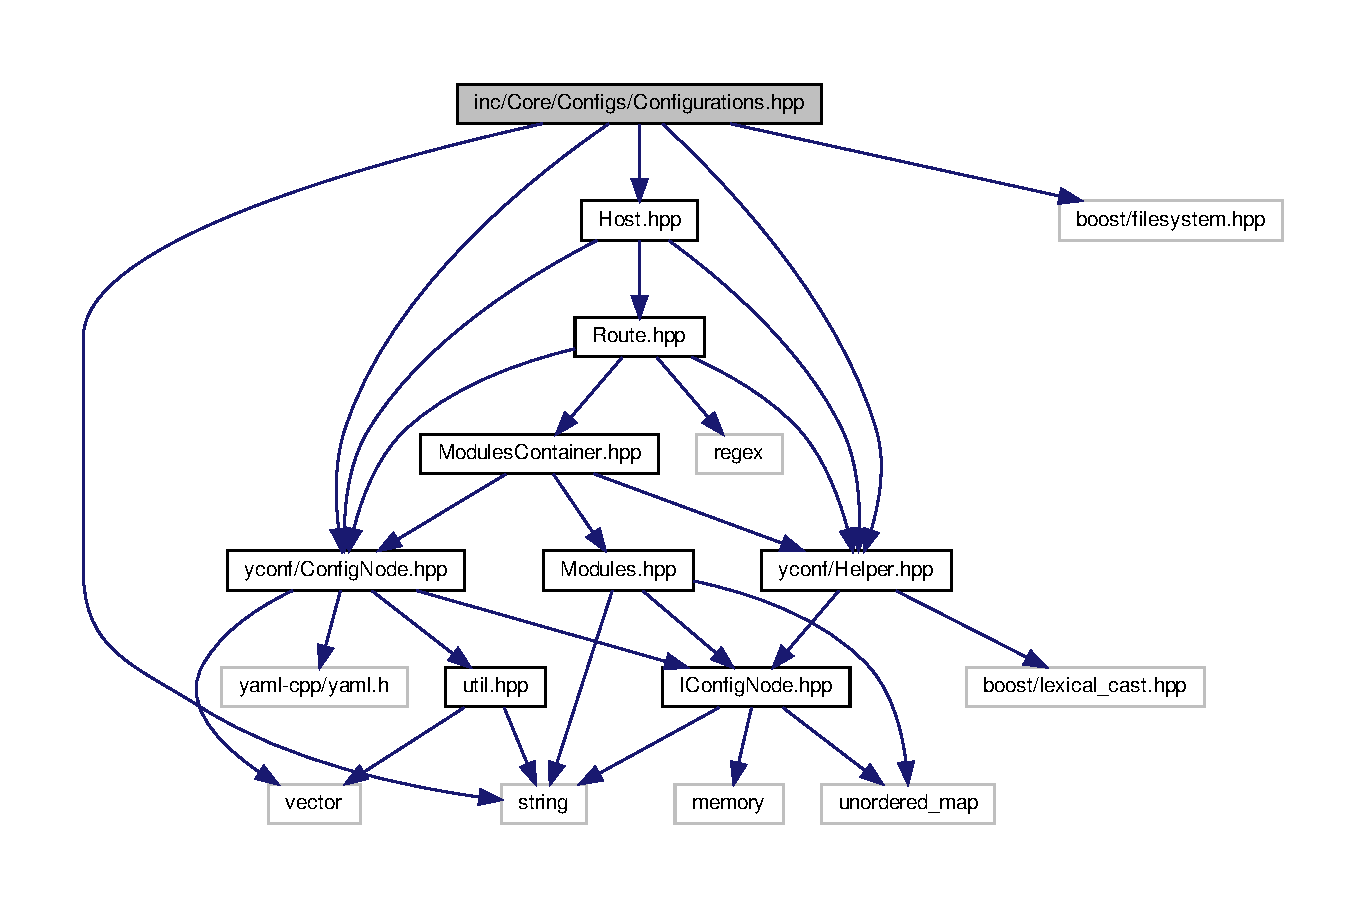
\includegraphics[width=350pt]{Configurations_8hpp__incl}
\end{center}
\end{figure}
This graph shows which files directly or indirectly include this file\+:
\nopagebreak
\begin{figure}[H]
\begin{center}
\leavevmode
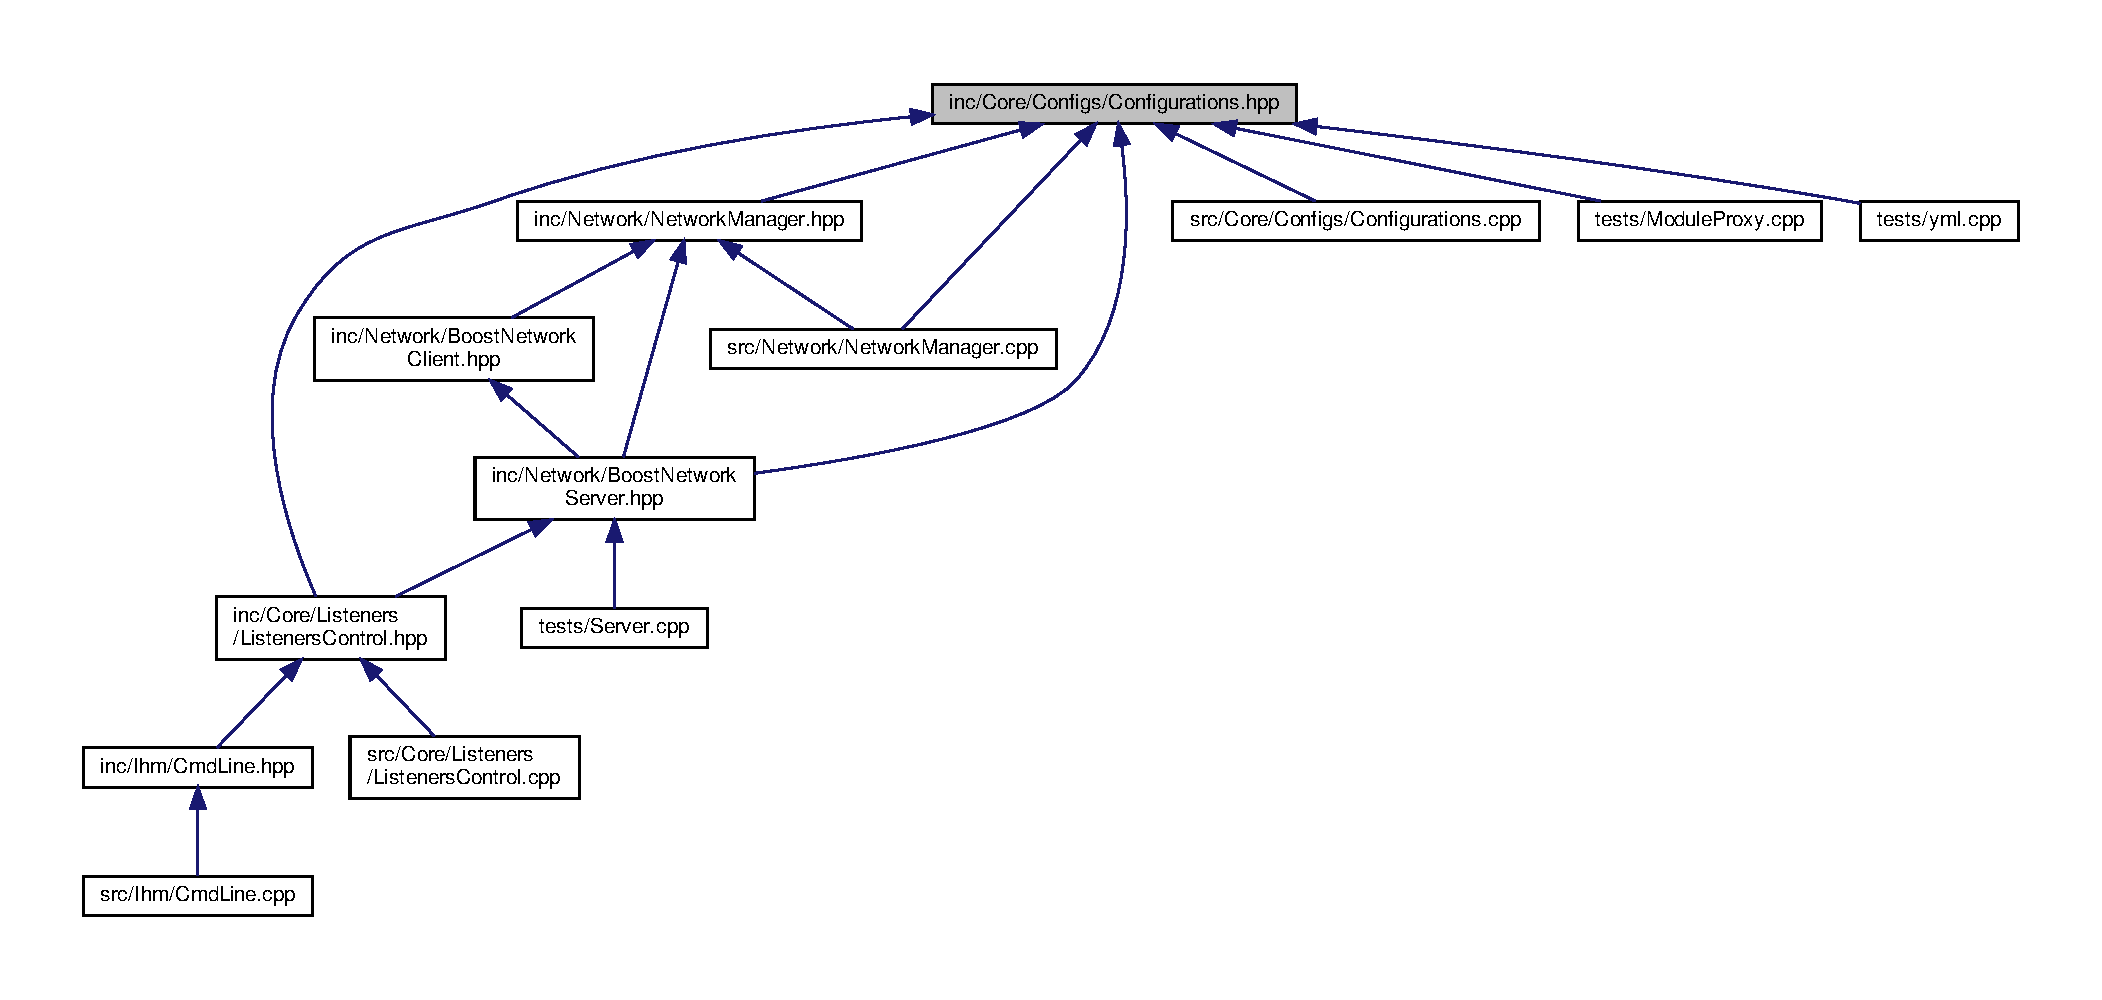
\includegraphics[width=350pt]{Configurations_8hpp__dep__incl}
\end{center}
\end{figure}
\subsection*{Classes}
\begin{DoxyCompactItemize}
\item 
class \hyperlink{classcore_1_1Configurations}{core\+::\+Configurations}
\end{DoxyCompactItemize}


\subsection{Detailed Description}
\begin{DoxyAuthor}{Author}
Gabriel Hamel (\href{mailto:gabriel.hamel@epitech.eu}{\tt gabriel.\+hamel@epitech.\+eu}) 
\end{DoxyAuthor}
\begin{DoxyVersion}{Version}
1.\+0 
\end{DoxyVersion}
\begin{DoxyDate}{Date}
2020-\/01-\/23
\end{DoxyDate}
\begin{DoxyCopyright}{Copyright}
Copyright (c) 2020 
\end{DoxyCopyright}

\hypertarget{Host_8hpp}{}\section{inc/\+Core/\+Configs/\+Host.hpp File Reference}
\label{Host_8hpp}\index{inc/\+Core/\+Configs/\+Host.\+hpp@{inc/\+Core/\+Configs/\+Host.\+hpp}}
{\ttfamily \#include \char`\"{}yconf/\+Config\+Node.\+hpp\char`\"{}}\newline
{\ttfamily \#include \char`\"{}yconf/\+Helper.\+hpp\char`\"{}}\newline
{\ttfamily \#include \char`\"{}Route.\+hpp\char`\"{}}\newline
Include dependency graph for Host.\+hpp\+:
\nopagebreak
\begin{figure}[H]
\begin{center}
\leavevmode
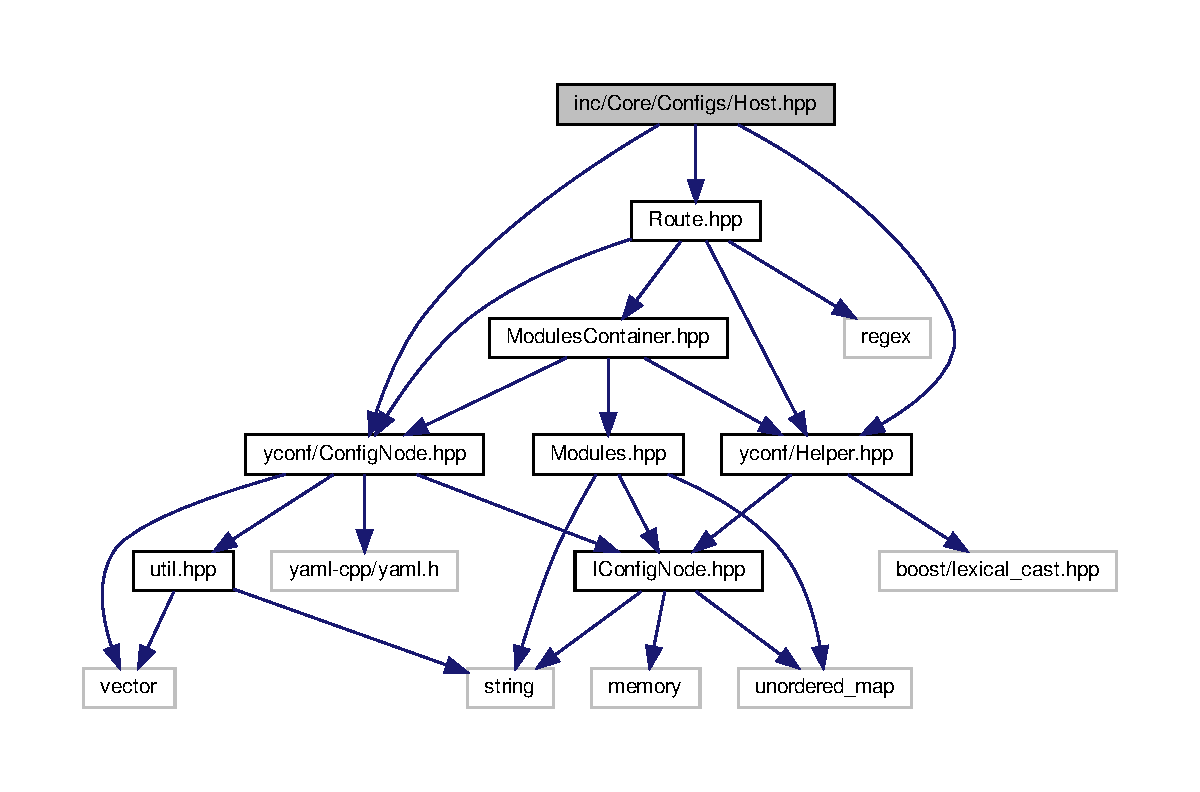
\includegraphics[width=350pt]{Host_8hpp__incl}
\end{center}
\end{figure}
This graph shows which files directly or indirectly include this file\+:
\nopagebreak
\begin{figure}[H]
\begin{center}
\leavevmode
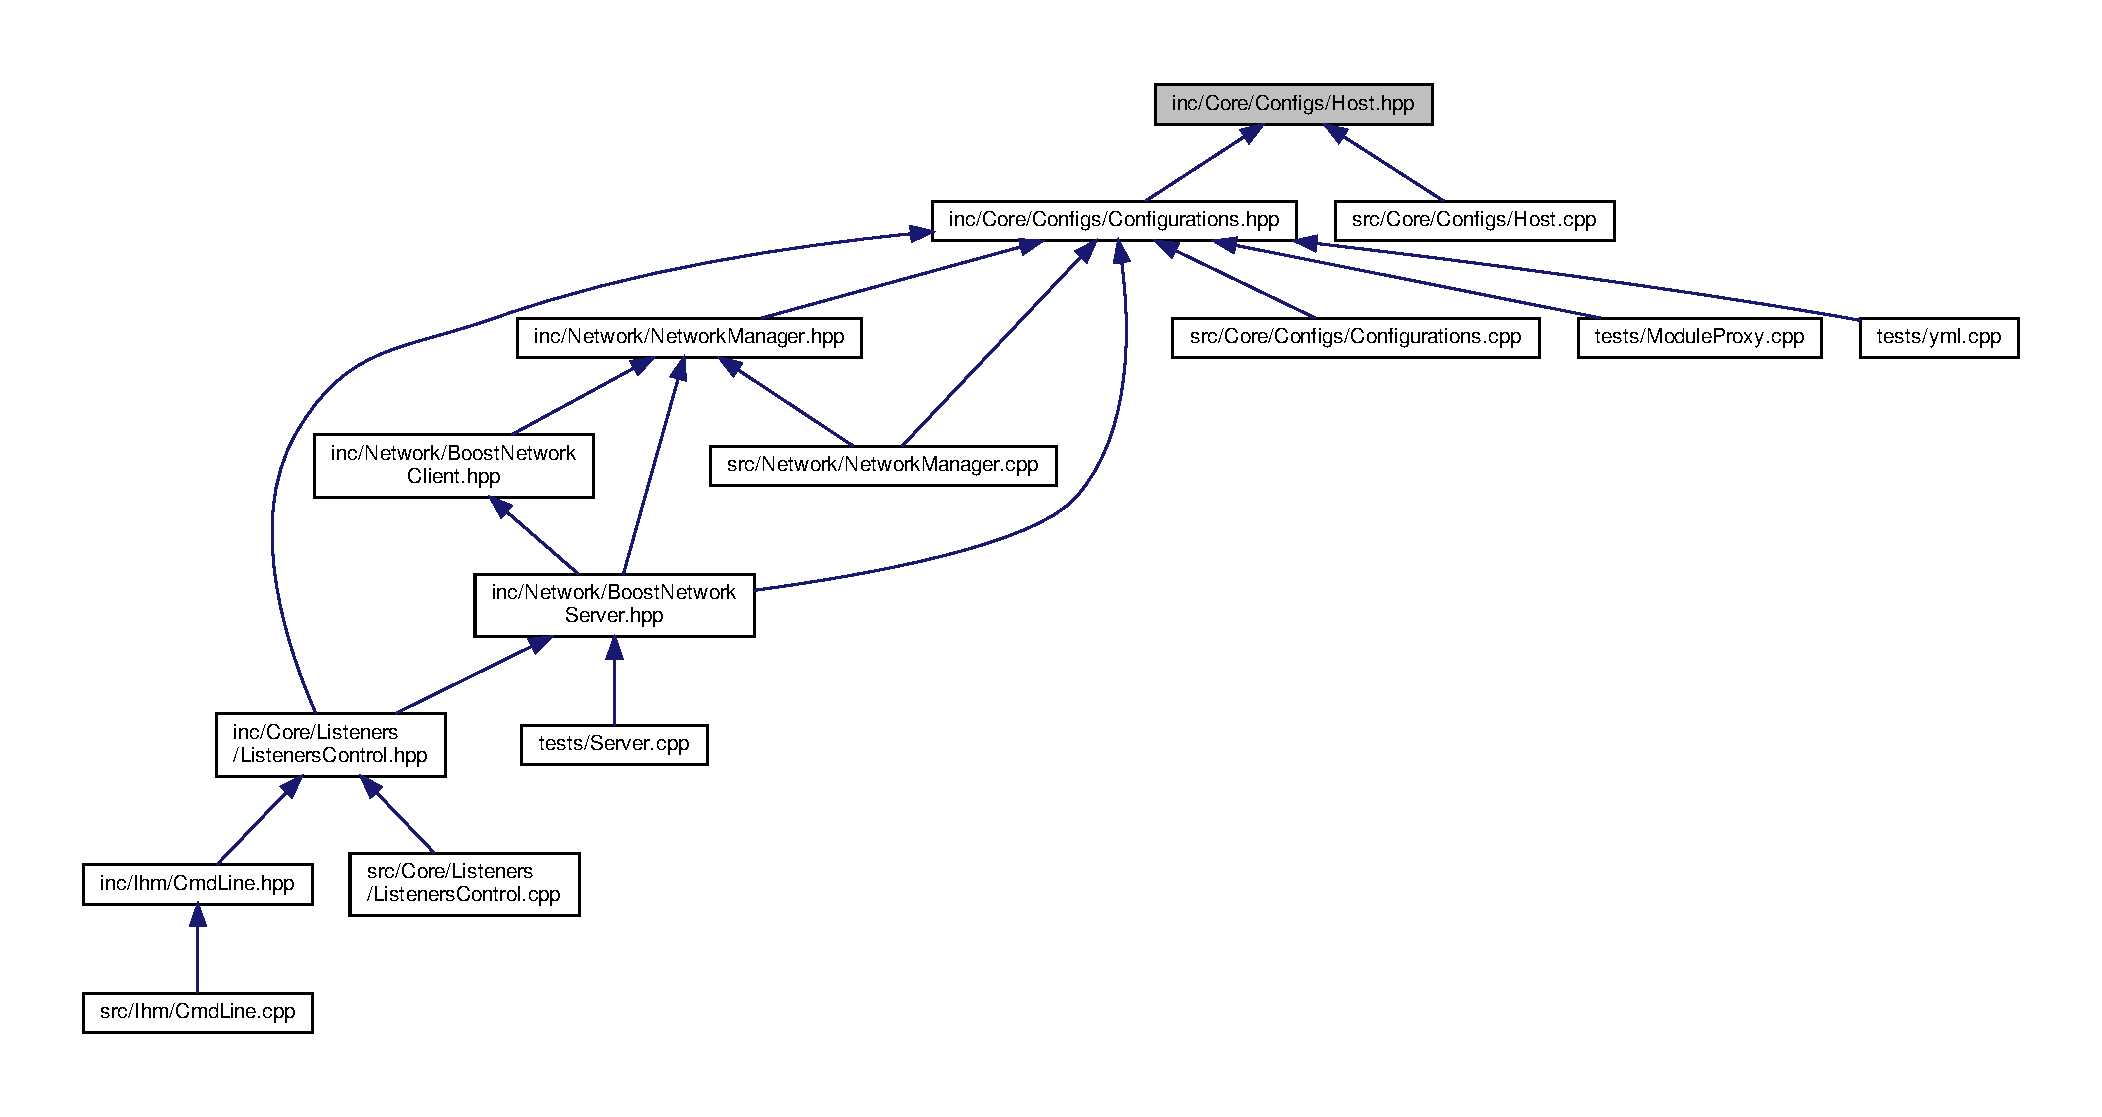
\includegraphics[width=350pt]{Host_8hpp__dep__incl}
\end{center}
\end{figure}
\subsection*{Classes}
\begin{DoxyCompactItemize}
\item 
class \hyperlink{classcore_1_1config_1_1Host}{core\+::config\+::\+Host}
\end{DoxyCompactItemize}


\subsection{Detailed Description}
\begin{DoxyAuthor}{Author}
Gabriel Hamel (\href{mailto:gabriel.hamel@epitech.eu}{\tt gabriel.\+hamel@epitech.\+eu}) 
\end{DoxyAuthor}
\begin{DoxyVersion}{Version}
1.\+0 
\end{DoxyVersion}
\begin{DoxyDate}{Date}
2020-\/01-\/25
\end{DoxyDate}
\begin{DoxyCopyright}{Copyright}
Copyright (c) 2020 
\end{DoxyCopyright}

\hypertarget{Modules_8hpp}{}\section{inc/\+Core/\+Configs/\+Modules.hpp File Reference}
\label{Modules_8hpp}\index{inc/\+Core/\+Configs/\+Modules.\+hpp@{inc/\+Core/\+Configs/\+Modules.\+hpp}}
{\ttfamily \#include $<$string$>$}\newline
{\ttfamily \#include $<$unordered\+\_\+map$>$}\newline
{\ttfamily \#include \char`\"{}I\+Config\+Node.\+hpp\char`\"{}}\newline
Include dependency graph for Modules.\+hpp\+:
\nopagebreak
\begin{figure}[H]
\begin{center}
\leavevmode
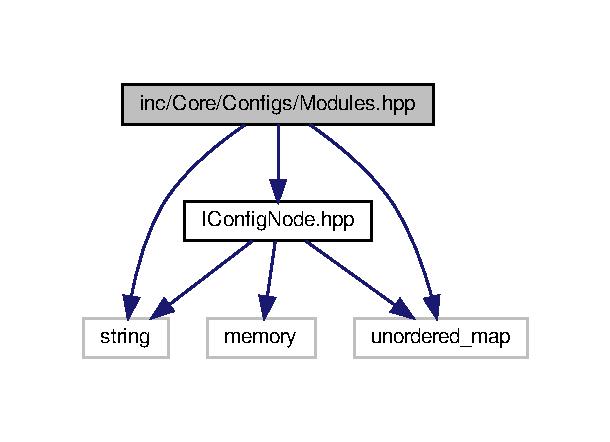
\includegraphics[width=293pt]{Modules_8hpp__incl}
\end{center}
\end{figure}
This graph shows which files directly or indirectly include this file\+:
\nopagebreak
\begin{figure}[H]
\begin{center}
\leavevmode
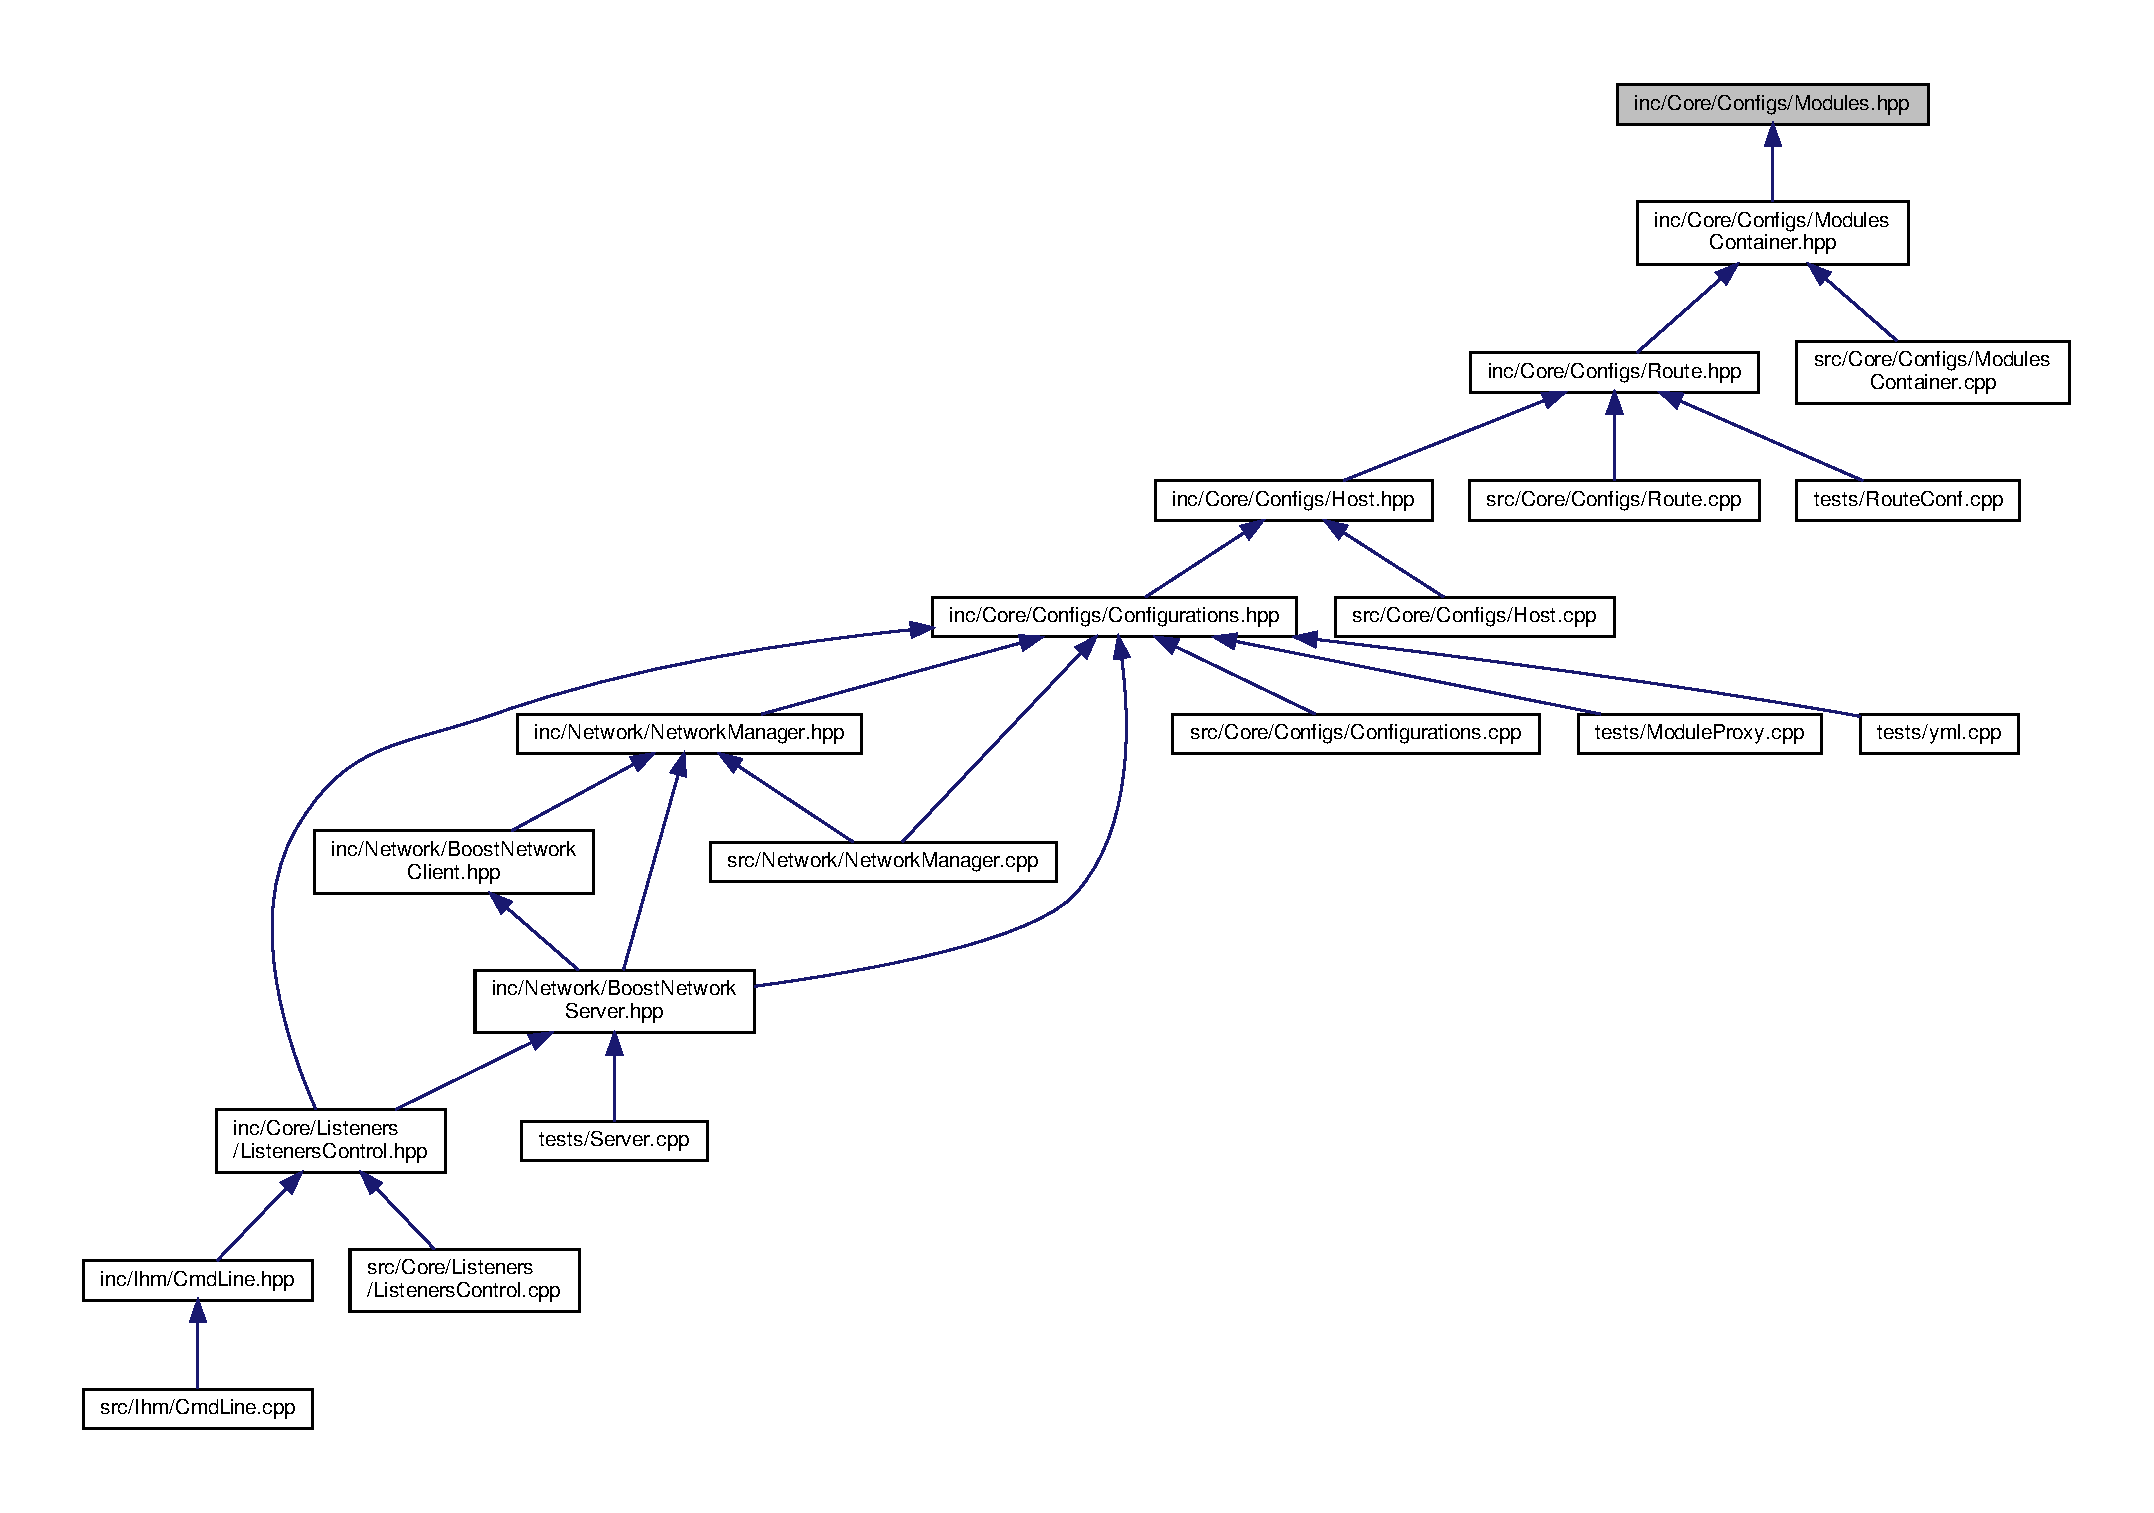
\includegraphics[width=350pt]{Modules_8hpp__dep__incl}
\end{center}
\end{figure}
\subsection*{Classes}
\begin{DoxyCompactItemize}
\item 
class \hyperlink{classcore_1_1config_1_1Module}{core\+::config\+::\+Module}
\end{DoxyCompactItemize}


\subsection{Detailed Description}
\begin{DoxyAuthor}{Author}
Gabriel Hamel (\href{mailto:gabriel.hamel.pro@epitech.eu}{\tt gabriel.\+hamel.\+pro@epitech.\+eu}) 
\end{DoxyAuthor}
\begin{DoxyVersion}{Version}
1.\+0 
\end{DoxyVersion}
\begin{DoxyDate}{Date}
2020-\/02-\/11
\end{DoxyDate}
\begin{DoxyCopyright}{Copyright}
Copyright (c) 2020 
\end{DoxyCopyright}

\hypertarget{ModulesContainer_8hpp}{}\section{inc/\+Core/\+Configs/\+Modules\+Container.hpp File Reference}
\label{ModulesContainer_8hpp}\index{inc/\+Core/\+Configs/\+Modules\+Container.\+hpp@{inc/\+Core/\+Configs/\+Modules\+Container.\+hpp}}
{\ttfamily \#include \char`\"{}yconf/\+Config\+Node.\+hpp\char`\"{}}\newline
{\ttfamily \#include \char`\"{}yconf/\+Helper.\+hpp\char`\"{}}\newline
{\ttfamily \#include \char`\"{}Modules.\+hpp\char`\"{}}\newline
Include dependency graph for Modules\+Container.\+hpp\+:
\nopagebreak
\begin{figure}[H]
\begin{center}
\leavevmode
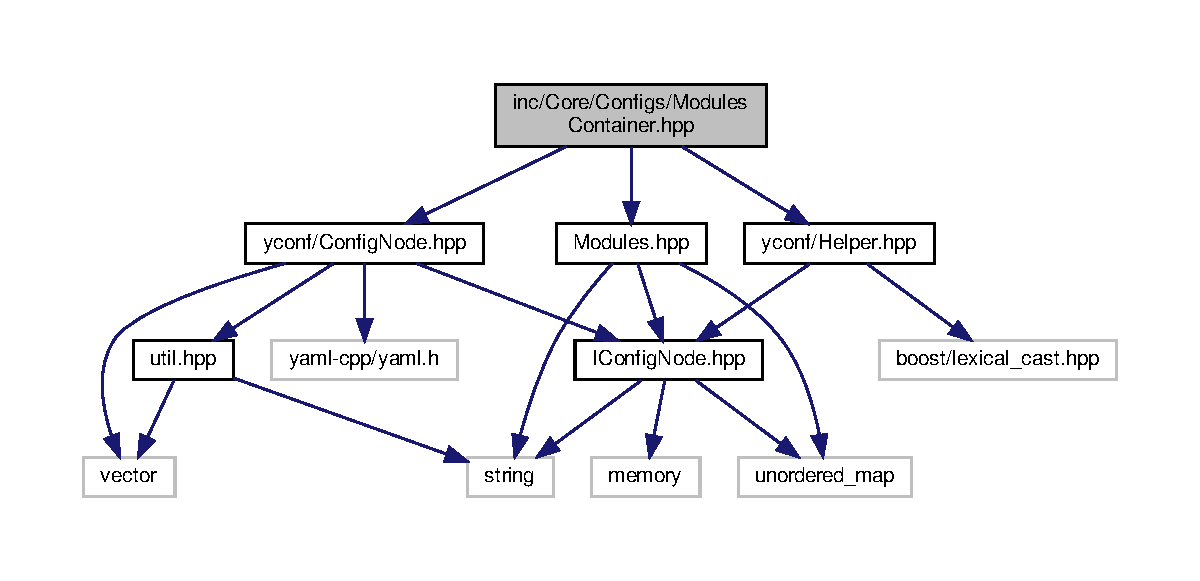
\includegraphics[width=350pt]{ModulesContainer_8hpp__incl}
\end{center}
\end{figure}
This graph shows which files directly or indirectly include this file\+:
\nopagebreak
\begin{figure}[H]
\begin{center}
\leavevmode
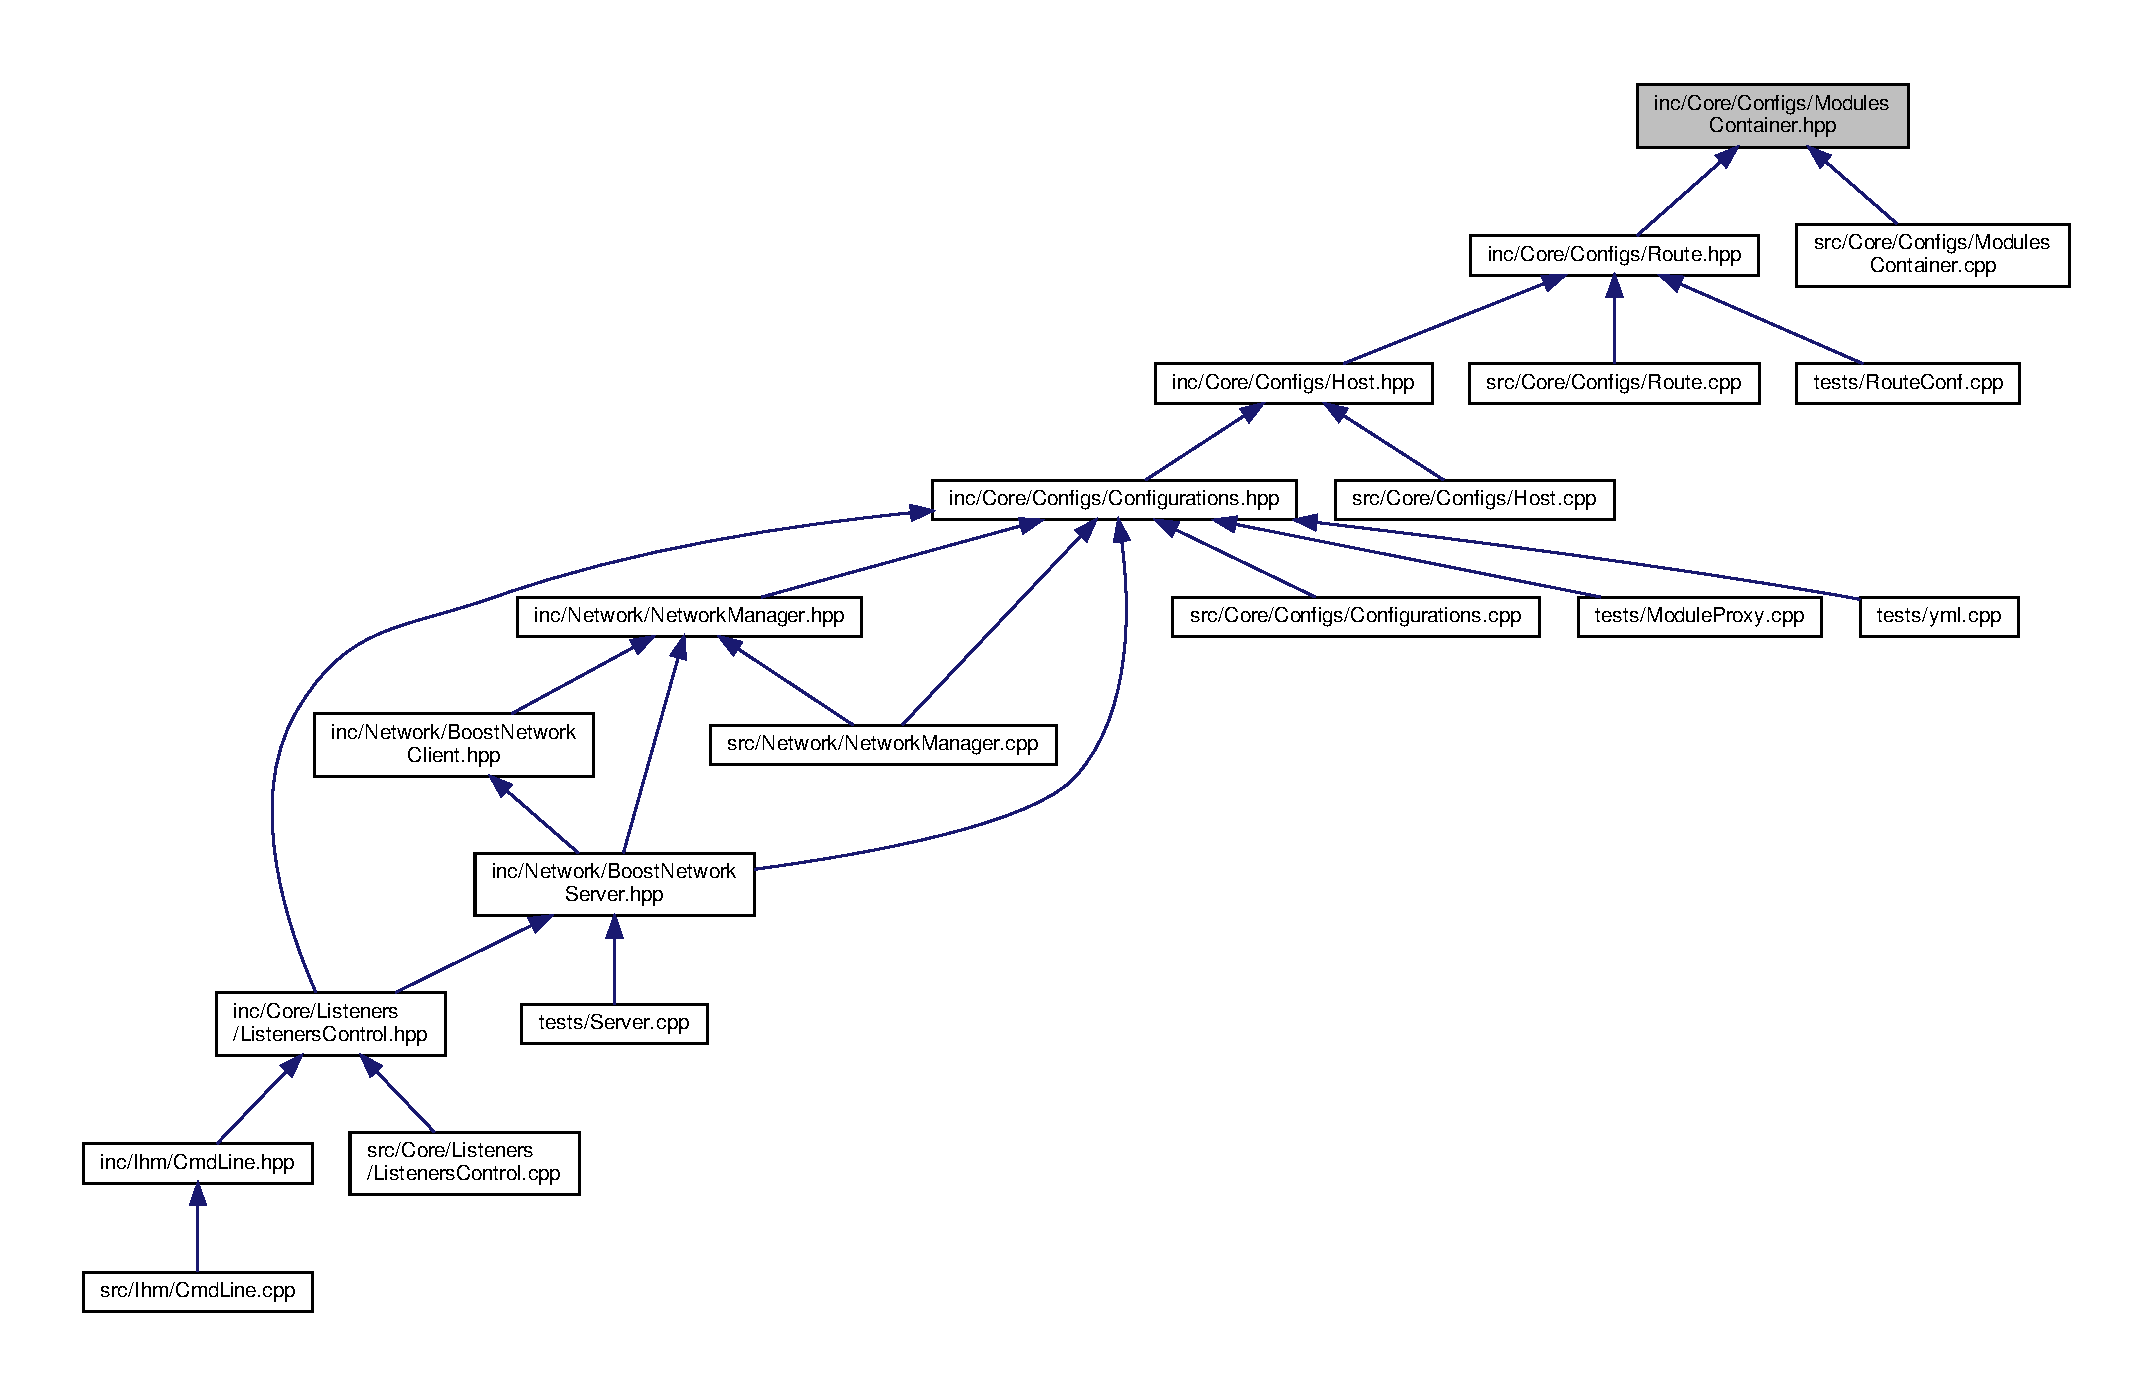
\includegraphics[width=350pt]{ModulesContainer_8hpp__dep__incl}
\end{center}
\end{figure}
\subsection*{Classes}
\begin{DoxyCompactItemize}
\item 
class \hyperlink{classcore_1_1config_1_1ModulesContainer}{core\+::config\+::\+Modules\+Container}
\end{DoxyCompactItemize}


\subsection{Detailed Description}
\begin{DoxyAuthor}{Author}
Gabriel Hamel (\href{mailto:gabriel.hamel@epitech.eu}{\tt gabriel.\+hamel@epitech.\+eu}) 
\end{DoxyAuthor}
\begin{DoxyVersion}{Version}
1.\+0 
\end{DoxyVersion}
\begin{DoxyDate}{Date}
2020-\/01-\/31
\end{DoxyDate}
\begin{DoxyCopyright}{Copyright}
Copyright (c) 2020 
\end{DoxyCopyright}

\hypertarget{Route_8hpp}{}\section{inc/\+Core/\+Configs/\+Route.hpp File Reference}
\label{Route_8hpp}\index{inc/\+Core/\+Configs/\+Route.\+hpp@{inc/\+Core/\+Configs/\+Route.\+hpp}}
{\ttfamily \#include $<$regex$>$}\newline
{\ttfamily \#include \char`\"{}yconf/\+Config\+Node.\+hpp\char`\"{}}\newline
{\ttfamily \#include \char`\"{}yconf/\+Helper.\+hpp\char`\"{}}\newline
{\ttfamily \#include \char`\"{}Modules\+Container.\+hpp\char`\"{}}\newline
Include dependency graph for Route.\+hpp\+:
\nopagebreak
\begin{figure}[H]
\begin{center}
\leavevmode
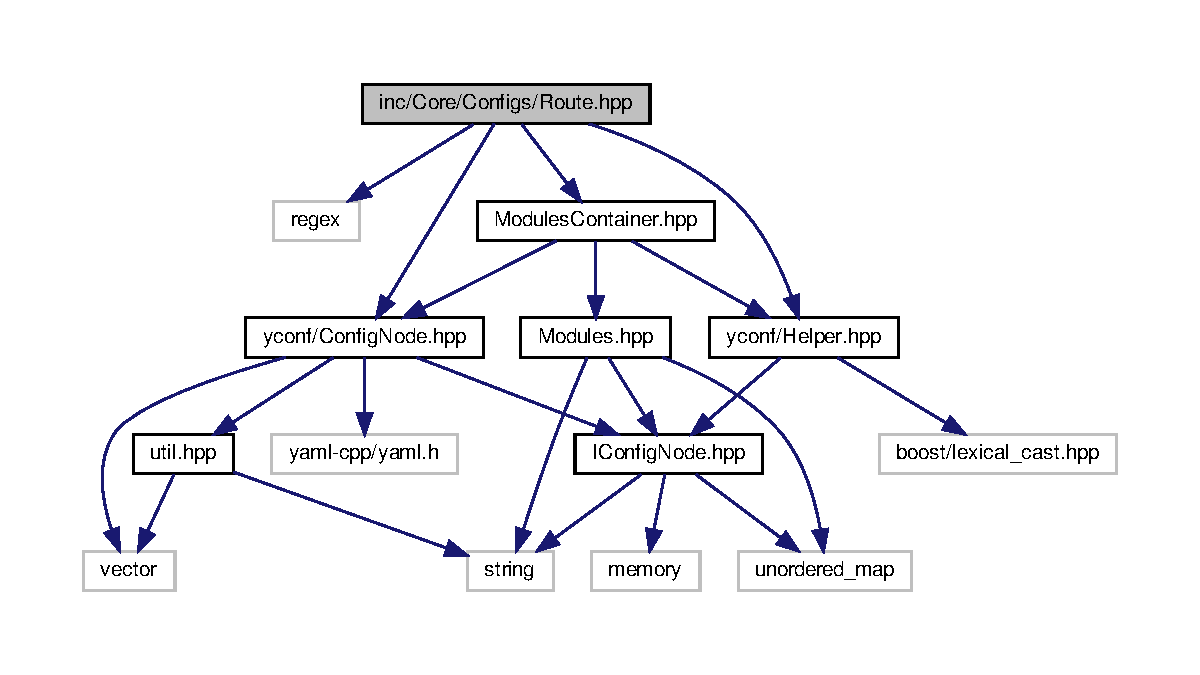
\includegraphics[width=350pt]{Route_8hpp__incl}
\end{center}
\end{figure}
This graph shows which files directly or indirectly include this file\+:
\nopagebreak
\begin{figure}[H]
\begin{center}
\leavevmode
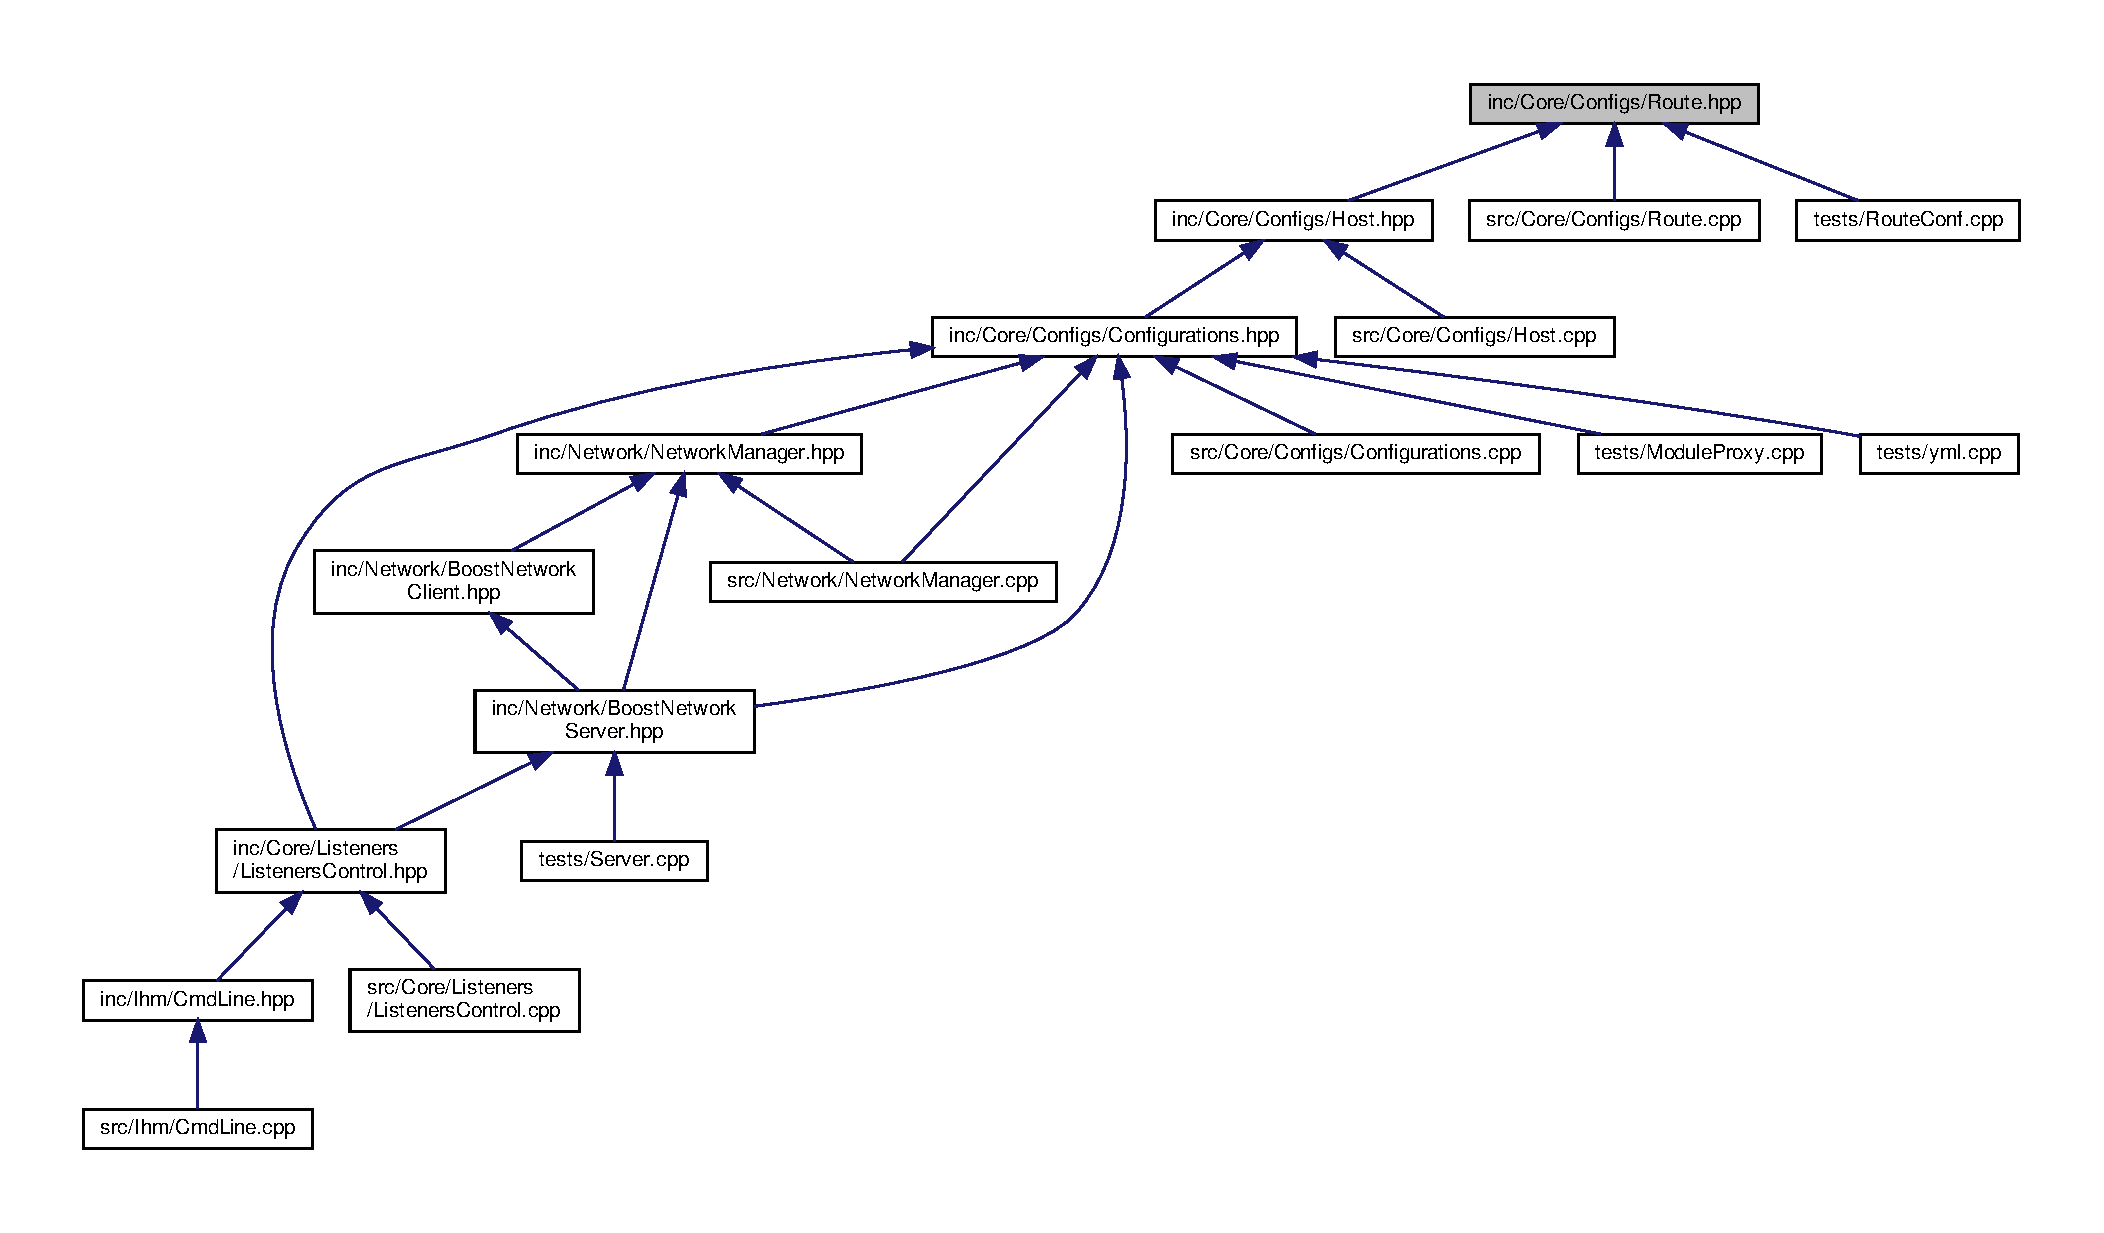
\includegraphics[width=350pt]{Route_8hpp__dep__incl}
\end{center}
\end{figure}
\subsection*{Classes}
\begin{DoxyCompactItemize}
\item 
class \hyperlink{classcore_1_1config_1_1Route}{core\+::config\+::\+Route}
\end{DoxyCompactItemize}


\subsection{Detailed Description}
\begin{DoxyAuthor}{Author}
Gabriel Hamel (\href{mailto:gabriel.hamel@epitech.eu}{\tt gabriel.\+hamel@epitech.\+eu}) 
\end{DoxyAuthor}
\begin{DoxyVersion}{Version}
1.\+0 
\end{DoxyVersion}
\begin{DoxyDate}{Date}
2020-\/01-\/28
\end{DoxyDate}
\begin{DoxyCopyright}{Copyright}
Copyright (c) 2020 
\end{DoxyCopyright}

\hypertarget{CmdLine_8hpp}{}\section{inc/\+Ihm/\+Cmd\+Line.hpp File Reference}
\label{CmdLine_8hpp}\index{inc/\+Ihm/\+Cmd\+Line.\+hpp@{inc/\+Ihm/\+Cmd\+Line.\+hpp}}
{\ttfamily \#include \char`\"{}Listeners\+Control.\+hpp\char`\"{}}\newline
Include dependency graph for Cmd\+Line.\+hpp\+:
\nopagebreak
\begin{figure}[H]
\begin{center}
\leavevmode
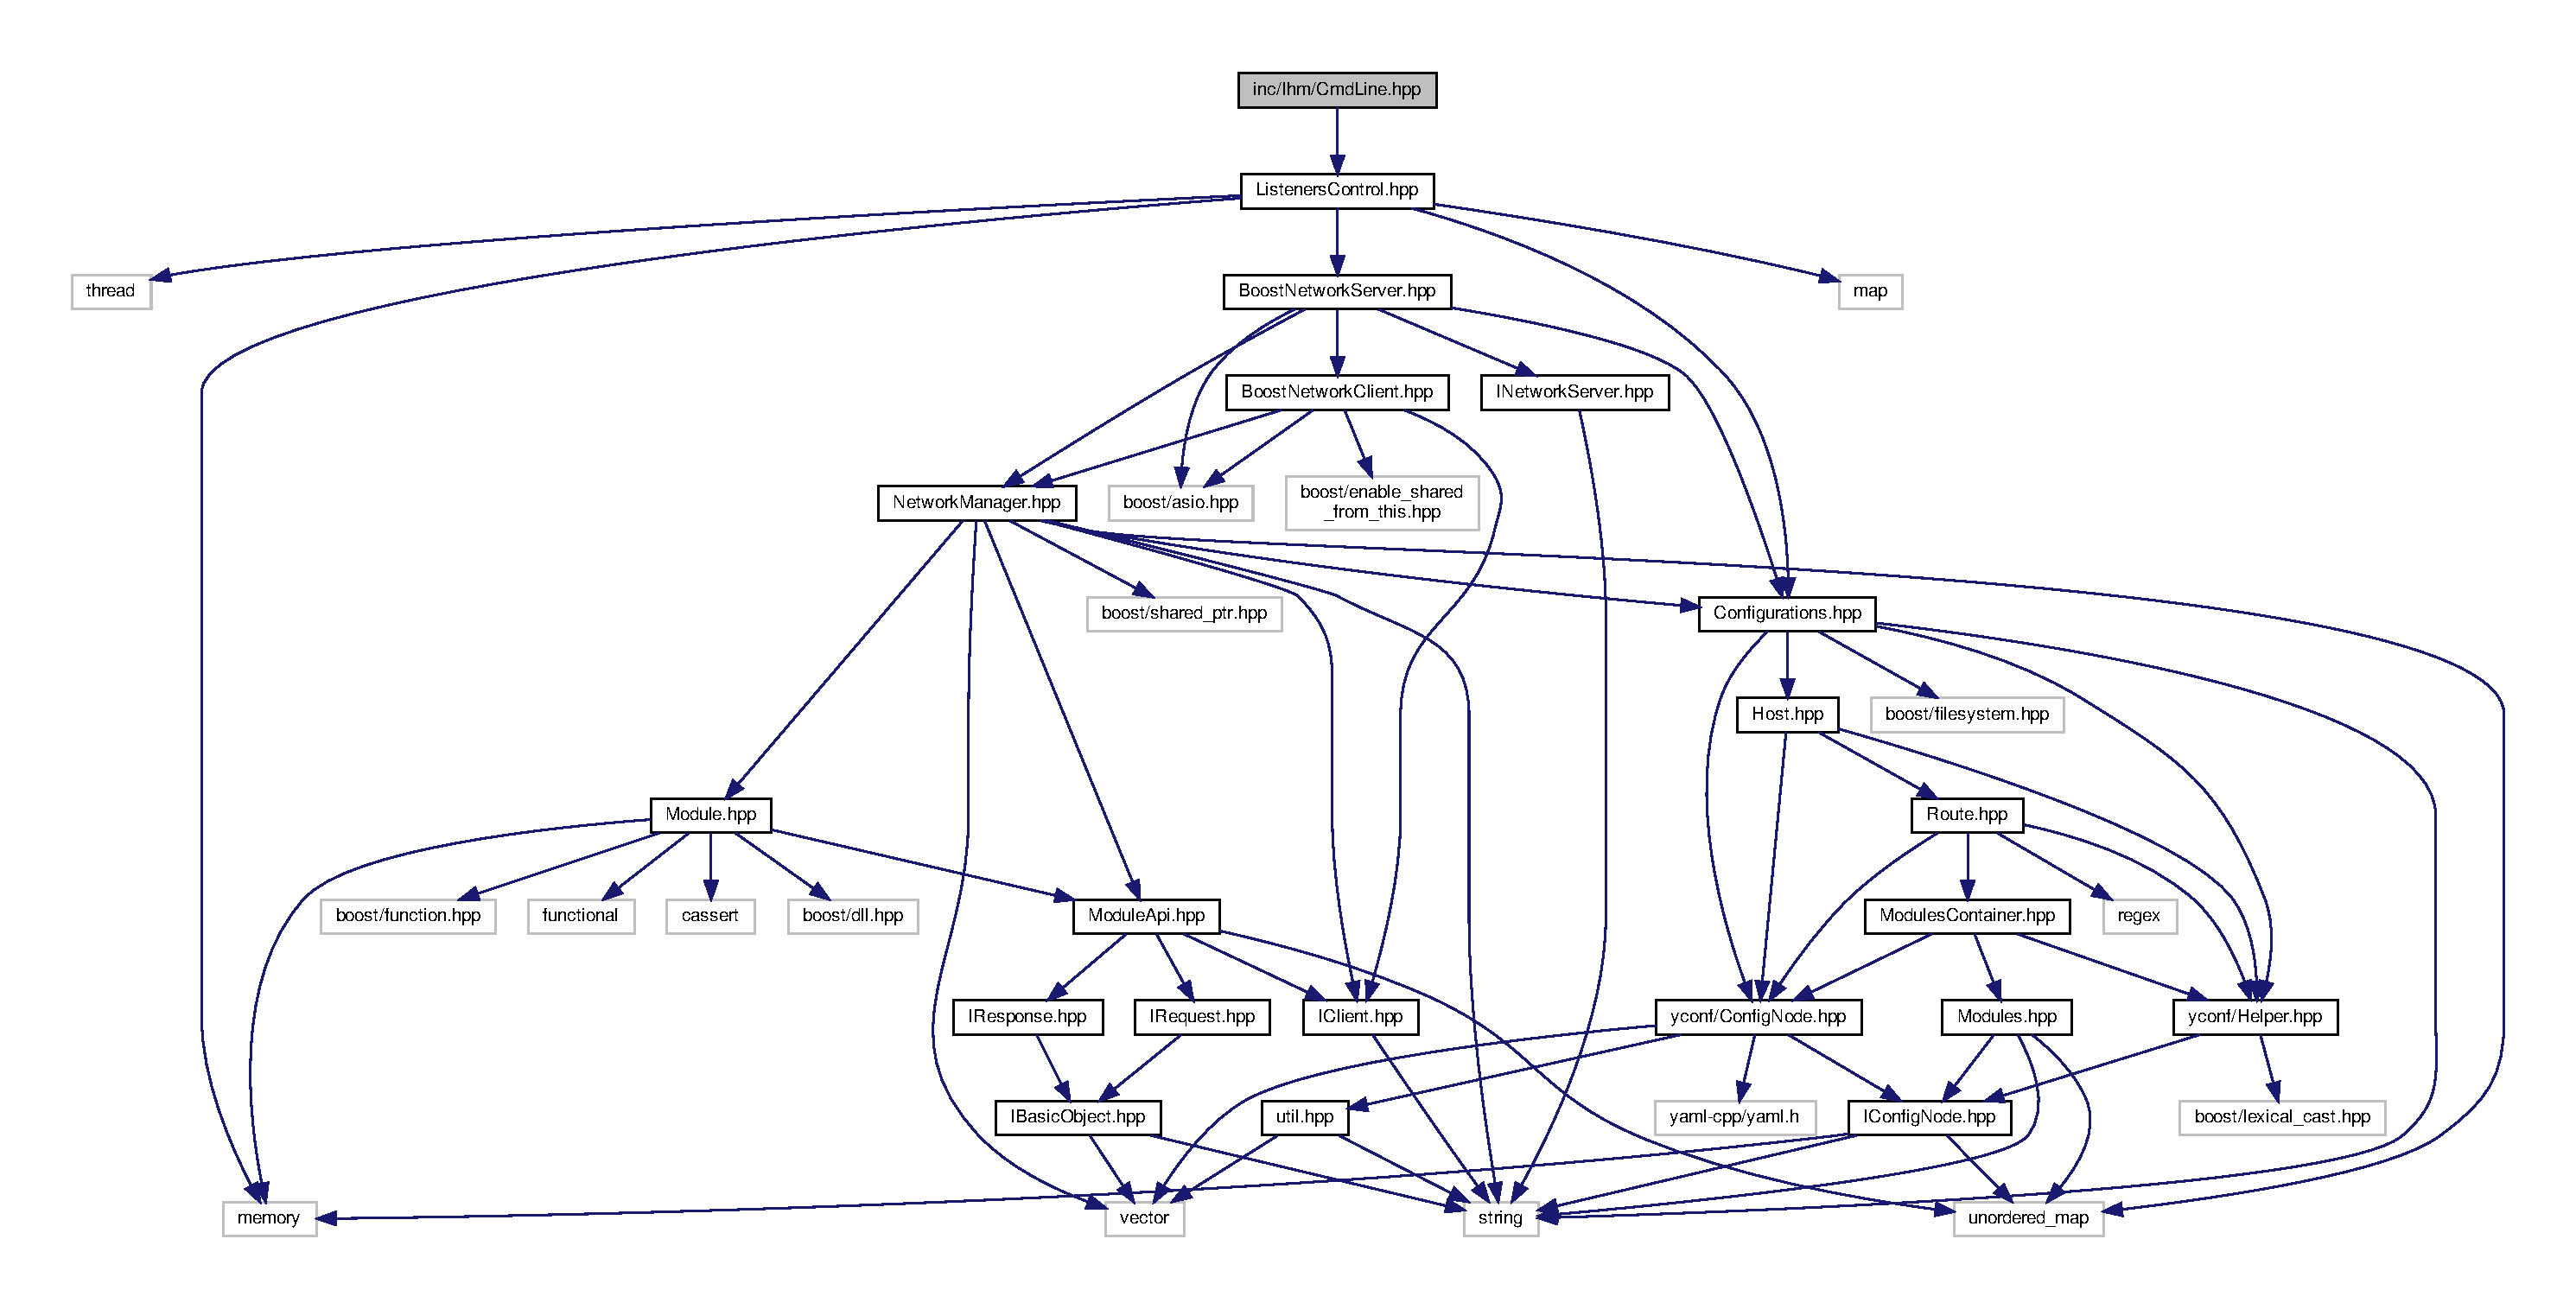
\includegraphics[width=350pt]{CmdLine_8hpp__incl}
\end{center}
\end{figure}
This graph shows which files directly or indirectly include this file\+:
\nopagebreak
\begin{figure}[H]
\begin{center}
\leavevmode
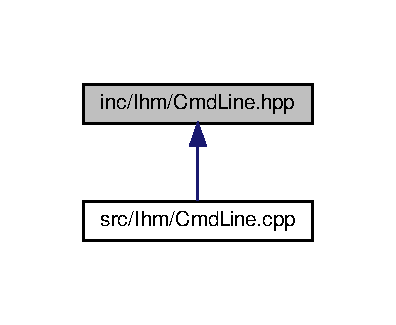
\includegraphics[width=190pt]{CmdLine_8hpp__dep__incl}
\end{center}
\end{figure}
\subsection*{Classes}
\begin{DoxyCompactItemize}
\item 
struct \hyperlink{structihm_1_1command__t}{ihm\+::command\+\_\+t}
\item 
class \hyperlink{classihm_1_1CmdLine}{ihm\+::\+Cmd\+Line}
\begin{DoxyCompactList}\small\item\em Interact with the user by tokenized string. \end{DoxyCompactList}\end{DoxyCompactItemize}


\subsection{Detailed Description}
\begin{DoxyAuthor}{Author}
Gabriel Hamel (\href{mailto:gabriel.hamel@epitech.eu}{\tt gabriel.\+hamel@epitech.\+eu}) 
\end{DoxyAuthor}
\begin{DoxyVersion}{Version}
1.\+0 
\end{DoxyVersion}
\begin{DoxyDate}{Date}
2020-\/01-\/23
\end{DoxyDate}
\begin{DoxyCopyright}{Copyright}
Copyright (c) 2020 
\end{DoxyCopyright}

\hypertarget{BoostNetworkClient_8hpp}{}\section{inc/\+Network/\+Boost\+Network\+Client.hpp File Reference}
\label{BoostNetworkClient_8hpp}\index{inc/\+Network/\+Boost\+Network\+Client.\+hpp@{inc/\+Network/\+Boost\+Network\+Client.\+hpp}}


An boost asio instance to store and comunicate with a network client.  


{\ttfamily \#include $<$boost/asio.\+hpp$>$}\newline
{\ttfamily \#include $<$boost/enable\+\_\+shared\+\_\+from\+\_\+this.\+hpp$>$}\newline
{\ttfamily \#include \char`\"{}I\+Client.\+hpp\char`\"{}}\newline
{\ttfamily \#include \char`\"{}Network\+Manager.\+hpp\char`\"{}}\newline
Include dependency graph for Boost\+Network\+Client.\+hpp\+:
\nopagebreak
\begin{figure}[H]
\begin{center}
\leavevmode
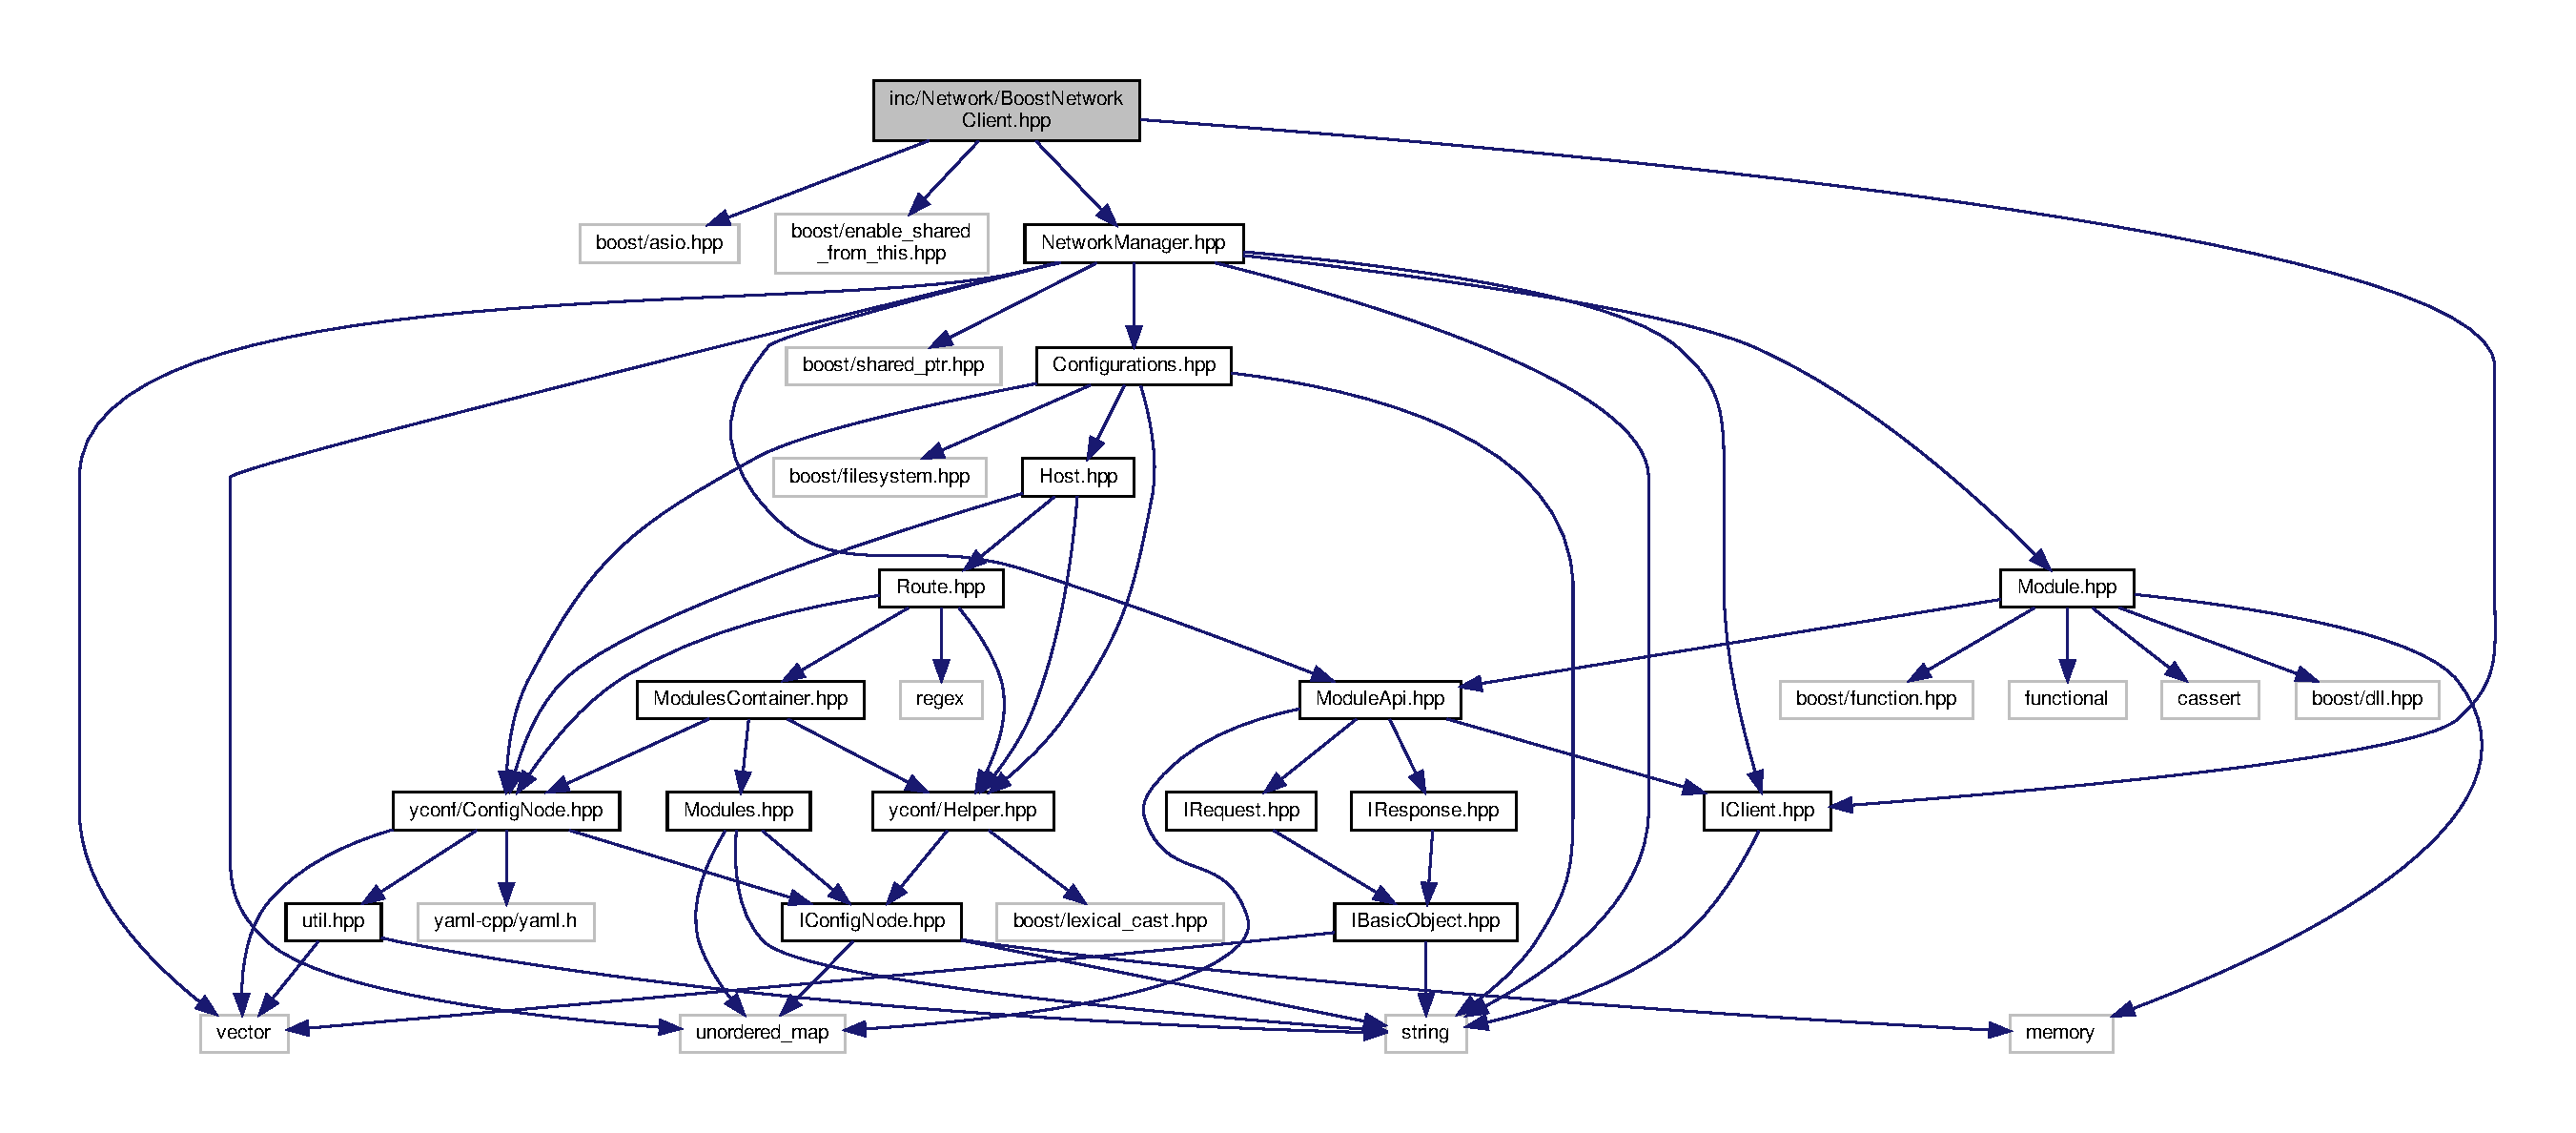
\includegraphics[width=350pt]{BoostNetworkClient_8hpp__incl}
\end{center}
\end{figure}
This graph shows which files directly or indirectly include this file\+:
\nopagebreak
\begin{figure}[H]
\begin{center}
\leavevmode
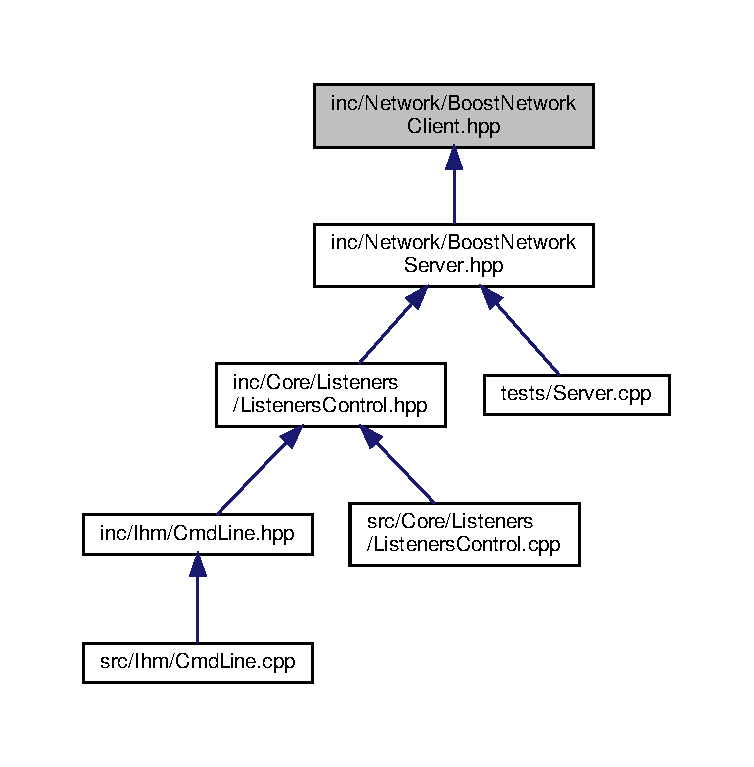
\includegraphics[width=350pt]{BoostNetworkClient_8hpp__dep__incl}
\end{center}
\end{figure}
\subsection*{Classes}
\begin{DoxyCompactItemize}
\item 
class \hyperlink{classnet_1_1BoostNetworkClient}{net\+::\+Boost\+Network\+Client}
\end{DoxyCompactItemize}


\subsection{Detailed Description}
An boost asio instance to store and comunicate with a network client. 

\begin{DoxyAuthor}{Author}
Gabriel Hamel (\href{mailto:gabriel.hamel@epitech.eu}{\tt gabriel.\+hamel@epitech.\+eu}) 
\end{DoxyAuthor}
\begin{DoxyVersion}{Version}
1.\+0 
\end{DoxyVersion}
\begin{DoxyDate}{Date}
2020-\/01-\/15
\end{DoxyDate}
\begin{DoxyCopyright}{Copyright}
Copyright (c) 2020 
\end{DoxyCopyright}

\hypertarget{BoostNetworkServer_8hpp}{}\section{inc/\+Network/\+Boost\+Network\+Server.hpp File Reference}
\label{BoostNetworkServer_8hpp}\index{inc/\+Network/\+Boost\+Network\+Server.\+hpp@{inc/\+Network/\+Boost\+Network\+Server.\+hpp}}


Boost encapsulation of the server tcp.  


{\ttfamily \#include $<$boost/asio.\+hpp$>$}\newline
{\ttfamily \#include \char`\"{}I\+Network\+Server.\+hpp\char`\"{}}\newline
{\ttfamily \#include \char`\"{}Network\+Manager.\+hpp\char`\"{}}\newline
{\ttfamily \#include \char`\"{}Boost\+Network\+Client.\+hpp\char`\"{}}\newline
{\ttfamily \#include \char`\"{}Configurations.\+hpp\char`\"{}}\newline
Include dependency graph for Boost\+Network\+Server.\+hpp\+:
\nopagebreak
\begin{figure}[H]
\begin{center}
\leavevmode
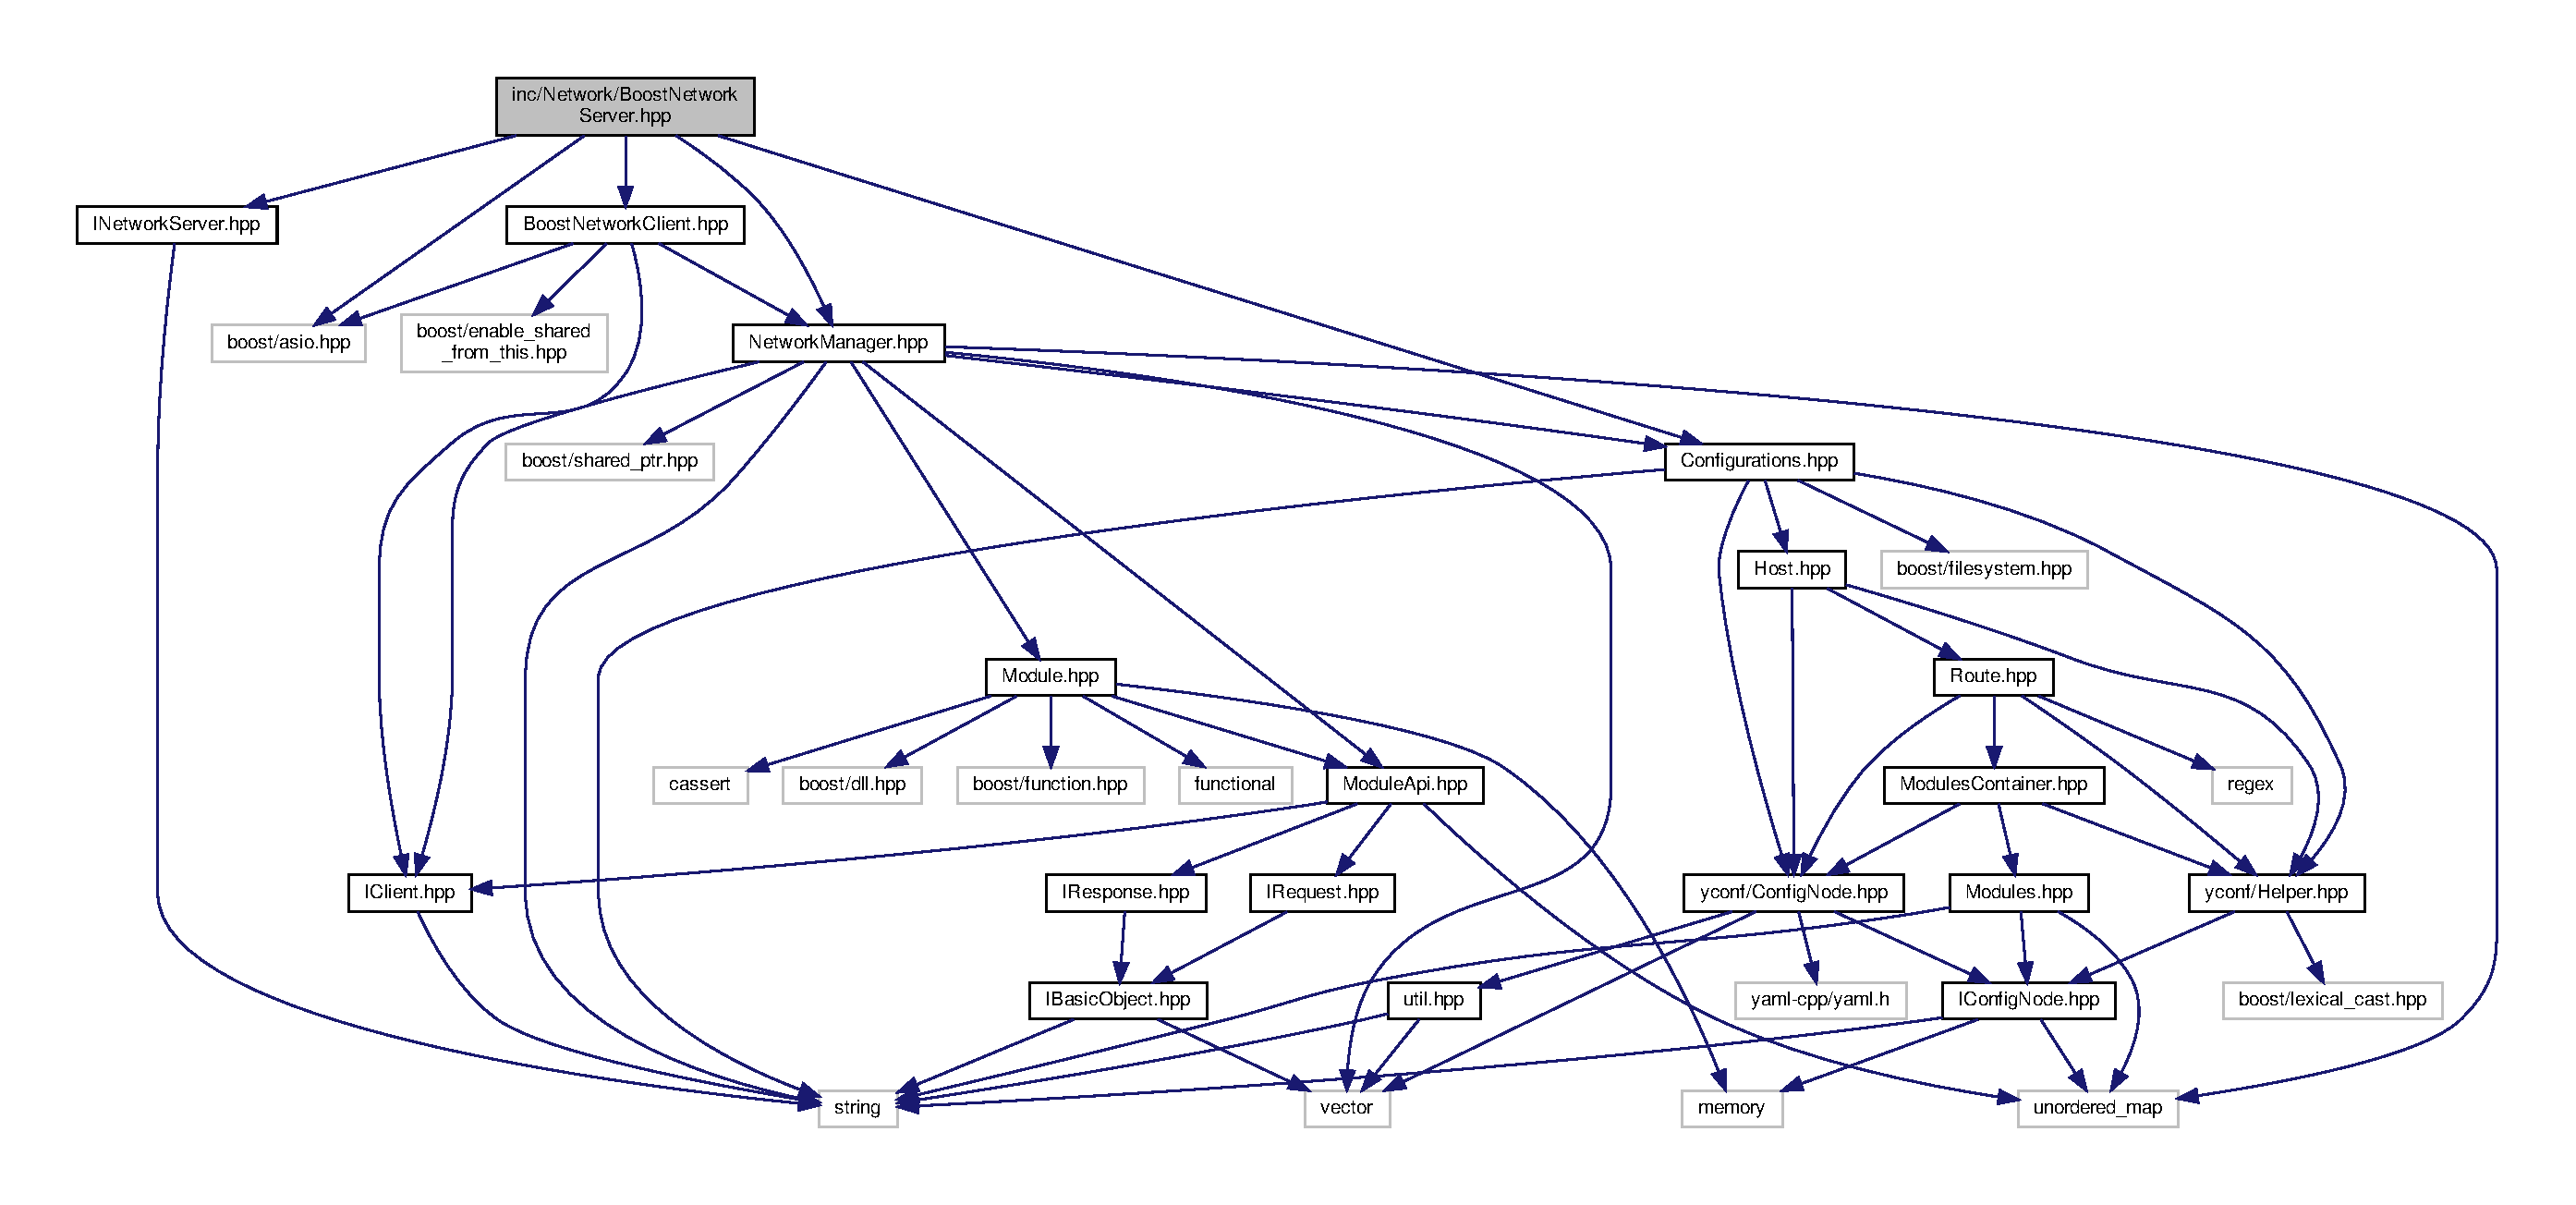
\includegraphics[width=350pt]{BoostNetworkServer_8hpp__incl}
\end{center}
\end{figure}
This graph shows which files directly or indirectly include this file\+:
\nopagebreak
\begin{figure}[H]
\begin{center}
\leavevmode
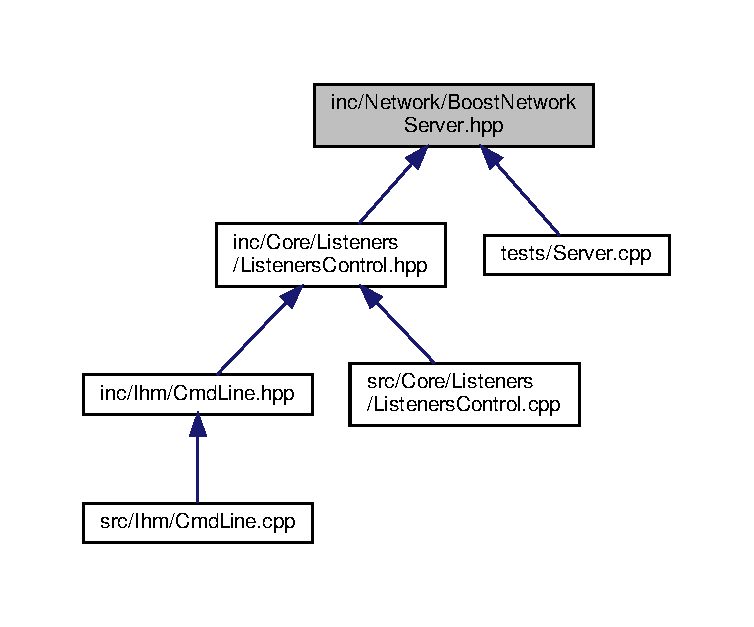
\includegraphics[width=350pt]{BoostNetworkServer_8hpp__dep__incl}
\end{center}
\end{figure}
\subsection*{Classes}
\begin{DoxyCompactItemize}
\item 
class \hyperlink{classnet_1_1BoostNetworkServer}{net\+::\+Boost\+Network\+Server}
\end{DoxyCompactItemize}


\subsection{Detailed Description}
Boost encapsulation of the server tcp. 

\begin{DoxyAuthor}{Author}
Gabriel Hamel (\href{mailto:gabriel.hamel@epitech.eu}{\tt gabriel.\+hamel@epitech.\+eu}) 
\end{DoxyAuthor}
\begin{DoxyVersion}{Version}
1.\+0 
\end{DoxyVersion}
\begin{DoxyDate}{Date}
2020-\/01-\/15
\end{DoxyDate}
\begin{DoxyCopyright}{Copyright}
Copyright (c) 2020 
\end{DoxyCopyright}

\hypertarget{INetworkServer_8hpp}{}\section{inc/\+Network/\+I\+Network\+Server.hpp File Reference}
\label{INetworkServer_8hpp}\index{inc/\+Network/\+I\+Network\+Server.\+hpp@{inc/\+Network/\+I\+Network\+Server.\+hpp}}


server interface  


{\ttfamily \#include $<$string$>$}\newline
Include dependency graph for I\+Network\+Server.\+hpp\+:
\nopagebreak
\begin{figure}[H]
\begin{center}
\leavevmode
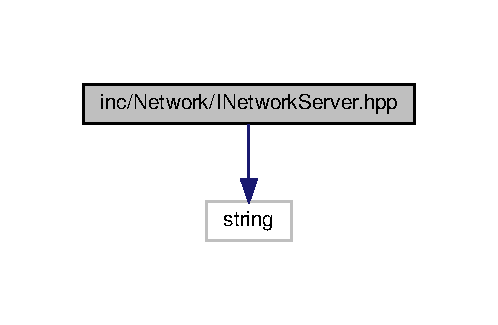
\includegraphics[width=239pt]{INetworkServer_8hpp__incl}
\end{center}
\end{figure}
This graph shows which files directly or indirectly include this file\+:
\nopagebreak
\begin{figure}[H]
\begin{center}
\leavevmode
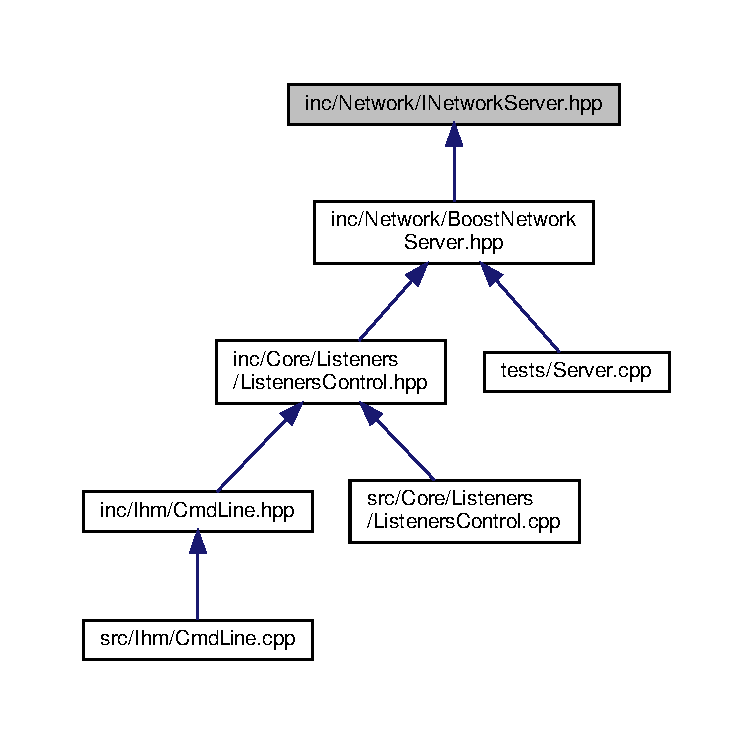
\includegraphics[width=350pt]{INetworkServer_8hpp__dep__incl}
\end{center}
\end{figure}
\subsection*{Classes}
\begin{DoxyCompactItemize}
\item 
class \hyperlink{classnet_1_1INetworkServer}{net\+::\+I\+Network\+Server}
\end{DoxyCompactItemize}


\subsection{Detailed Description}
server interface 

\begin{DoxyAuthor}{Author}
Gabriel Hamel (\href{mailto:gabriel.hamel@epitech.eu}{\tt gabriel.\+hamel@epitech.\+eu}) 
\end{DoxyAuthor}
\begin{DoxyVersion}{Version}
1.\+0 
\end{DoxyVersion}
\begin{DoxyDate}{Date}
2020-\/01-\/15
\end{DoxyDate}
\begin{DoxyCopyright}{Copyright}
Copyright (c) 2020 
\end{DoxyCopyright}

\hypertarget{NetworkManager_8hpp}{}\section{inc/\+Network/\+Network\+Manager.hpp File Reference}
\label{NetworkManager_8hpp}\index{inc/\+Network/\+Network\+Manager.\+hpp@{inc/\+Network/\+Network\+Manager.\+hpp}}


Class to interract with network part and worker.  


{\ttfamily \#include $<$string$>$}\newline
{\ttfamily \#include $<$vector$>$}\newline
{\ttfamily \#include $<$boost/shared\+\_\+ptr.\+hpp$>$}\newline
{\ttfamily \#include $<$unordered\+\_\+map$>$}\newline
{\ttfamily \#include \char`\"{}I\+Client.\+hpp\char`\"{}}\newline
{\ttfamily \#include \char`\"{}Configurations.\+hpp\char`\"{}}\newline
{\ttfamily \#include \char`\"{}Module\+Api.\+hpp\char`\"{}}\newline
{\ttfamily \#include \char`\"{}Module.\+hpp\char`\"{}}\newline
Include dependency graph for Network\+Manager.\+hpp\+:
\nopagebreak
\begin{figure}[H]
\begin{center}
\leavevmode
\includegraphics[width=350pt]{NetworkManager_8hpp__incl}
\end{center}
\end{figure}
This graph shows which files directly or indirectly include this file\+:
\nopagebreak
\begin{figure}[H]
\begin{center}
\leavevmode
\includegraphics[width=350pt]{NetworkManager_8hpp__dep__incl}
\end{center}
\end{figure}
\subsection*{Classes}
\begin{DoxyCompactItemize}
\item 
class \hyperlink{classnet_1_1NetworkManager}{net\+::\+Network\+Manager}
\end{DoxyCompactItemize}


\subsection{Detailed Description}
Class to interract with network part and worker. 

\begin{DoxyAuthor}{Author}
Gabriel Hamel (\href{mailto:gabriel.hamel@epitech.eu}{\tt gabriel.\+hamel@epitech.\+eu}) 
\end{DoxyAuthor}
\begin{DoxyVersion}{Version}
1.\+0 
\end{DoxyVersion}
\begin{DoxyDate}{Date}
2020-\/01-\/15
\end{DoxyDate}
\begin{DoxyCopyright}{Copyright}
Copyright (c) 2020 
\end{DoxyCopyright}

\hypertarget{File_8cpp}{}\section{modules/\+File/\+File.cpp File Reference}
\label{File_8cpp}\index{modules/\+File/\+File.\+cpp@{modules/\+File/\+File.\+cpp}}


An basic module who say hello at each requests.  


{\ttfamily \#include $<$boost/dll/alias.\+hpp$>$}\newline
{\ttfamily \#include $<$iostream$>$}\newline
{\ttfamily \#include $<$sstream$>$}\newline
{\ttfamily \#include $<$fstream$>$}\newline
{\ttfamily \#include $<$boost/filesystem.\+hpp$>$}\newline
{\ttfamily \#include $<$algorithm$>$}\newline
{\ttfamily \#include $<$regex$>$}\newline
{\ttfamily \#include $<$unordered\+\_\+map$>$}\newline
{\ttfamily \#include \char`\"{}File.\+hpp\char`\"{}}\newline
Include dependency graph for File.\+cpp\+:
\nopagebreak
\begin{figure}[H]
\begin{center}
\leavevmode
\includegraphics[width=350pt]{File_8cpp__incl}
\end{center}
\end{figure}
\subsection*{Functions}
\begin{DoxyCompactItemize}
\item 
\mbox{\Hypertarget{File_8cpp_a9aed91b9158795989084578060857bcc}\label{File_8cpp_a9aed91b9158795989084578060857bcc}} 
\hyperlink{structmodule_1_1Api}{module\+::\+Api} $\ast$ {\bfseries factory} ()
\end{DoxyCompactItemize}


\subsection{Detailed Description}
An basic module who say hello at each requests. 

\begin{DoxyAuthor}{Author}
Gabriel Hamel (\href{mailto:gabriel.hamel.pro@gmail.com}{\tt gabriel.\+hamel.\+pro@gmail.\+com}) 
\end{DoxyAuthor}
\begin{DoxyVersion}{Version}
1.\+0 
\end{DoxyVersion}
\begin{DoxyDate}{Date}
2020-\/02-\/17
\end{DoxyDate}
\begin{DoxyCopyright}{Copyright}
Copyright (c) 2020 
\end{DoxyCopyright}

\hypertarget{File_8hpp}{}\section{modules/\+File/\+File.hpp File Reference}
\label{File_8hpp}\index{modules/\+File/\+File.\+hpp@{modules/\+File/\+File.\+hpp}}


An basic module who say hello at each requests.  


{\ttfamily \#include \char`\"{}Module\+Api.\+hpp\char`\"{}}\newline
Include dependency graph for File.\+hpp\+:
\nopagebreak
\begin{figure}[H]
\begin{center}
\leavevmode
\includegraphics[width=350pt]{File_8hpp__incl}
\end{center}
\end{figure}
This graph shows which files directly or indirectly include this file\+:
\nopagebreak
\begin{figure}[H]
\begin{center}
\leavevmode
\includegraphics[width=190pt]{File_8hpp__dep__incl}
\end{center}
\end{figure}
\subsection*{Classes}
\begin{DoxyCompactItemize}
\item 
class \hyperlink{classmodule_1_1File}{module\+::\+File}
\end{DoxyCompactItemize}


\subsection{Detailed Description}
An basic module who say hello at each requests. 

\begin{DoxyAuthor}{Author}
Gabriel Hamel (\href{mailto:gabriel.hamel.pro@gmail.com}{\tt gabriel.\+hamel.\+pro@gmail.\+com}) 
\end{DoxyAuthor}
\begin{DoxyVersion}{Version}
1.\+0 
\end{DoxyVersion}
\begin{DoxyDate}{Date}
2020-\/02-\/17
\end{DoxyDate}
\begin{DoxyCopyright}{Copyright}
Copyright (c) 2020 
\end{DoxyCopyright}

\hypertarget{Php_8cpp}{}\section{modules/\+Php/\+Php.cpp File Reference}
\label{Php_8cpp}\index{modules/\+Php/\+Php.\+cpp@{modules/\+Php/\+Php.\+cpp}}
{\ttfamily \#include $<$boost/dll/alias.\+hpp$>$}\newline
{\ttfamily \#include $<$iostream$>$}\newline
{\ttfamily \#include $<$sstream$>$}\newline
{\ttfamily \#include $<$fstream$>$}\newline
{\ttfamily \#include $<$boost/filesystem.\+hpp$>$}\newline
{\ttfamily \#include $<$algorithm$>$}\newline
{\ttfamily \#include $<$regex$>$}\newline
{\ttfamily \#include $<$stdio.\+h$>$}\newline
{\ttfamily \#include \char`\"{}Php.\+hpp\char`\"{}}\newline
Include dependency graph for Php.\+cpp\+:
\nopagebreak
\begin{figure}[H]
\begin{center}
\leavevmode
\includegraphics[width=350pt]{Php_8cpp__incl}
\end{center}
\end{figure}
\subsection*{Functions}
\begin{DoxyCompactItemize}
\item 
\mbox{\Hypertarget{Php_8cpp_a9aed91b9158795989084578060857bcc}\label{Php_8cpp_a9aed91b9158795989084578060857bcc}} 
\hyperlink{structmodule_1_1Api}{module\+::\+Api} $\ast$ {\bfseries factory} ()
\end{DoxyCompactItemize}


\subsection{Detailed Description}
\begin{DoxyAuthor}{Author}
Gabriel Hamel (\href{mailto:gabriel.hamel.pro@gmail.com}{\tt gabriel.\+hamel.\+pro@gmail.\+com}) 
\end{DoxyAuthor}
\begin{DoxyVersion}{Version}
1.\+0 
\end{DoxyVersion}
\begin{DoxyDate}{Date}
2020-\/02-\/20
\end{DoxyDate}
\begin{DoxyCopyright}{Copyright}
Copyright (c) 2020 
\end{DoxyCopyright}

\hypertarget{Php_8hpp}{}\section{modules/\+Php/\+Php.hpp File Reference}
\label{Php_8hpp}\index{modules/\+Php/\+Php.\+hpp@{modules/\+Php/\+Php.\+hpp}}


An basic module who say hello at each requests.  


{\ttfamily \#include \char`\"{}Module\+Api.\+hpp\char`\"{}}\newline
Include dependency graph for Php.\+hpp\+:
\nopagebreak
\begin{figure}[H]
\begin{center}
\leavevmode
\includegraphics[width=350pt]{Php_8hpp__incl}
\end{center}
\end{figure}
This graph shows which files directly or indirectly include this file\+:
\nopagebreak
\begin{figure}[H]
\begin{center}
\leavevmode
\includegraphics[width=193pt]{Php_8hpp__dep__incl}
\end{center}
\end{figure}
\subsection*{Classes}
\begin{DoxyCompactItemize}
\item 
class \hyperlink{classmodule_1_1Php}{module\+::\+Php}
\end{DoxyCompactItemize}


\subsection{Detailed Description}
An basic module who say hello at each requests. 

\begin{DoxyAuthor}{Author}
Gabriel Hamel (\href{mailto:gabriel.hamel.pro@gmail.com}{\tt gabriel.\+hamel.\+pro@gmail.\+com}) 
\end{DoxyAuthor}
\begin{DoxyVersion}{Version}
1.\+0 
\end{DoxyVersion}
\begin{DoxyDate}{Date}
2020-\/02-\/17
\end{DoxyDate}
\begin{DoxyCopyright}{Copyright}
Copyright (c) 2020 
\end{DoxyCopyright}

\hypertarget{Proxy_8cpp}{}\section{modules/\+Proxy/\+Proxy.cpp File Reference}
\label{Proxy_8cpp}\index{modules/\+Proxy/\+Proxy.\+cpp@{modules/\+Proxy/\+Proxy.\+cpp}}
{\ttfamily \#include $<$boost/dll.\+hpp$>$}\newline
{\ttfamily \#include $<$iostream$>$}\newline
{\ttfamily \#include $<$sstream$>$}\newline
{\ttfamily \#include \char`\"{}Http\+Response.\+hpp\char`\"{}}\newline
{\ttfamily \#include \char`\"{}Proxy.\+hpp\char`\"{}}\newline
Include dependency graph for Proxy.\+cpp\+:
\nopagebreak
\begin{figure}[H]
\begin{center}
\leavevmode
\includegraphics[width=350pt]{Proxy_8cpp__incl}
\end{center}
\end{figure}
\subsection*{Functions}
\begin{DoxyCompactItemize}
\item 
\mbox{\Hypertarget{Proxy_8cpp_a9aed91b9158795989084578060857bcc}\label{Proxy_8cpp_a9aed91b9158795989084578060857bcc}} 
\hyperlink{structmodule_1_1Api}{module\+::\+Api} $\ast$ {\bfseries factory} ()
\end{DoxyCompactItemize}


\subsection{Detailed Description}
\begin{DoxyAuthor}{Author}
Gabriel Hamel (\href{mailto:gabriel.hamel.pro@gmail.com}{\tt gabriel.\+hamel.\+pro@gmail.\+com}) 
\end{DoxyAuthor}
\begin{DoxyVersion}{Version}
1.\+0 
\end{DoxyVersion}
\begin{DoxyDate}{Date}
2020-\/02-\/25
\end{DoxyDate}
\begin{DoxyCopyright}{Copyright}
Copyright (c) 2020 
\end{DoxyCopyright}

\hypertarget{Proxy_8hpp}{}\section{modules/\+Proxy/\+Proxy.hpp File Reference}
\label{Proxy_8hpp}\index{modules/\+Proxy/\+Proxy.\+hpp@{modules/\+Proxy/\+Proxy.\+hpp}}
{\ttfamily \#include \char`\"{}Module\+Api.\+hpp\char`\"{}}\newline
{\ttfamily \#include $<$boost/asio.\+hpp$>$}\newline
Include dependency graph for Proxy.\+hpp\+:
\nopagebreak
\begin{figure}[H]
\begin{center}
\leavevmode
\includegraphics[width=350pt]{Proxy_8hpp__incl}
\end{center}
\end{figure}
This graph shows which files directly or indirectly include this file\+:
\nopagebreak
\begin{figure}[H]
\begin{center}
\leavevmode
\includegraphics[width=209pt]{Proxy_8hpp__dep__incl}
\end{center}
\end{figure}
\subsection*{Classes}
\begin{DoxyCompactItemize}
\item 
class \hyperlink{classmodule_1_1Proxy}{module\+::\+Proxy}
\end{DoxyCompactItemize}


\subsection{Detailed Description}
\begin{DoxyAuthor}{Author}
Gabriel Hamel (\href{mailto:gabriel.hamel.pro@gmail.com}{\tt gabriel.\+hamel.\+pro@gmail.\+com}) 
\end{DoxyAuthor}
\begin{DoxyVersion}{Version}
1.\+0 
\end{DoxyVersion}
\begin{DoxyDate}{Date}
2020-\/02-\/25
\end{DoxyDate}
\begin{DoxyCopyright}{Copyright}
Copyright (c) 2020 
\end{DoxyCopyright}

\hypertarget{Configurations_8cpp}{}\section{src/\+Core/\+Configs/\+Configurations.cpp File Reference}
\label{Configurations_8cpp}\index{src/\+Core/\+Configs/\+Configurations.\+cpp@{src/\+Core/\+Configs/\+Configurations.\+cpp}}
{\ttfamily \#include $<$iostream$>$}\newline
{\ttfamily \#include $<$mutex$>$}\newline
{\ttfamily \#include \char`\"{}Configurations.\+hpp\char`\"{}}\newline
{\ttfamily \#include $<$boost/dll.\+hpp$>$}\newline
{\ttfamily \#include $<$boost/foreach.\+hpp$>$}\newline
Include dependency graph for Configurations.\+cpp\+:
\nopagebreak
\begin{figure}[H]
\begin{center}
\leavevmode
\includegraphics[width=350pt]{Configurations_8cpp__incl}
\end{center}
\end{figure}


\subsection{Detailed Description}
\begin{DoxyAuthor}{Author}
Gabriel Hamel (\href{mailto:gabriel.hamel@epitech.eu}{\tt gabriel.\+hamel@epitech.\+eu}) 
\end{DoxyAuthor}
\begin{DoxyVersion}{Version}
1.\+0 
\end{DoxyVersion}
\begin{DoxyDate}{Date}
2020-\/01-\/23
\end{DoxyDate}
\begin{DoxyCopyright}{Copyright}
Copyright (c) 2020 
\end{DoxyCopyright}

\hypertarget{Host_8cpp}{}\section{src/\+Core/\+Configs/\+Host.cpp File Reference}
\label{Host_8cpp}\index{src/\+Core/\+Configs/\+Host.\+cpp@{src/\+Core/\+Configs/\+Host.\+cpp}}
{\ttfamily \#include \char`\"{}Host.\+hpp\char`\"{}}\newline
Include dependency graph for Host.\+cpp\+:
\nopagebreak
\begin{figure}[H]
\begin{center}
\leavevmode
\includegraphics[width=350pt]{Host_8cpp__incl}
\end{center}
\end{figure}


\subsection{Detailed Description}
\begin{DoxyAuthor}{Author}
Gabriel Hamel (\href{mailto:gabriel.hamel@epitech.eu}{\tt gabriel.\+hamel@epitech.\+eu}) 
\end{DoxyAuthor}
\begin{DoxyVersion}{Version}
1.\+0 
\end{DoxyVersion}
\begin{DoxyDate}{Date}
2020-\/01-\/31
\end{DoxyDate}
\begin{DoxyCopyright}{Copyright}
Copyright (c) 2020 
\end{DoxyCopyright}

\hypertarget{ModulesContainer_8cpp}{}\section{src/\+Core/\+Configs/\+Modules\+Container.cpp File Reference}
\label{ModulesContainer_8cpp}\index{src/\+Core/\+Configs/\+Modules\+Container.\+cpp@{src/\+Core/\+Configs/\+Modules\+Container.\+cpp}}
{\ttfamily \#include \char`\"{}Modules\+Container.\+hpp\char`\"{}}\newline
Include dependency graph for Modules\+Container.\+cpp\+:
\nopagebreak
\begin{figure}[H]
\begin{center}
\leavevmode
\includegraphics[width=350pt]{ModulesContainer_8cpp__incl}
\end{center}
\end{figure}


\subsection{Detailed Description}
\begin{DoxyAuthor}{Author}
Gabriel Hamel (\href{mailto:gabriel.hamel@epitech.eu}{\tt gabriel.\+hamel@epitech.\+eu}) 
\end{DoxyAuthor}
\begin{DoxyVersion}{Version}
1.\+0 
\end{DoxyVersion}
\begin{DoxyDate}{Date}
2020-\/01-\/31
\end{DoxyDate}
\begin{DoxyCopyright}{Copyright}
Copyright (c) 2020 
\end{DoxyCopyright}

\hypertarget{Route_8cpp}{}\section{src/\+Core/\+Configs/\+Route.cpp File Reference}
\label{Route_8cpp}\index{src/\+Core/\+Configs/\+Route.\+cpp@{src/\+Core/\+Configs/\+Route.\+cpp}}
{\ttfamily \#include \char`\"{}Route.\+hpp\char`\"{}}\newline
Include dependency graph for Route.\+cpp\+:
\nopagebreak
\begin{figure}[H]
\begin{center}
\leavevmode
\includegraphics[width=350pt]{Route_8cpp__incl}
\end{center}
\end{figure}


\subsection{Detailed Description}
\begin{DoxyAuthor}{Author}
Gabriel Hamel (\href{mailto:gabriel.hamel@epitech.eu}{\tt gabriel.\+hamel@epitech.\+eu}) 
\end{DoxyAuthor}
\begin{DoxyVersion}{Version}
1.\+0 
\end{DoxyVersion}
\begin{DoxyDate}{Date}
2020-\/01-\/28
\end{DoxyDate}
\begin{DoxyCopyright}{Copyright}
Copyright (c) 2020 
\end{DoxyCopyright}

\hypertarget{ListenersControl_8cpp}{}\section{src/\+Core/\+Listeners/\+Listeners\+Control.cpp File Reference}
\label{ListenersControl_8cpp}\index{src/\+Core/\+Listeners/\+Listeners\+Control.\+cpp@{src/\+Core/\+Listeners/\+Listeners\+Control.\+cpp}}
{\ttfamily \#include $<$iostream$>$}\newline
{\ttfamily \#include \char`\"{}Listeners\+Control.\+hpp\char`\"{}}\newline
Include dependency graph for Listeners\+Control.\+cpp\+:
\nopagebreak
\begin{figure}[H]
\begin{center}
\leavevmode
\includegraphics[width=350pt]{ListenersControl_8cpp__incl}
\end{center}
\end{figure}


\subsection{Detailed Description}
\begin{DoxyAuthor}{Author}
Gabriel Hamel (\href{mailto:gabriel.hamel@epitech.eu}{\tt gabriel.\+hamel@epitech.\+eu}) 
\end{DoxyAuthor}
\begin{DoxyVersion}{Version}
1.\+0 
\end{DoxyVersion}
\begin{DoxyDate}{Date}
2020-\/01-\/23
\end{DoxyDate}
\begin{DoxyCopyright}{Copyright}
Copyright (c) 2020 
\end{DoxyCopyright}

\hypertarget{CmdLine_8cpp}{}\section{src/\+Ihm/\+Cmd\+Line.cpp File Reference}
\label{CmdLine_8cpp}\index{src/\+Ihm/\+Cmd\+Line.\+cpp@{src/\+Ihm/\+Cmd\+Line.\+cpp}}
{\ttfamily \#include $<$iostream$>$}\newline
{\ttfamily \#include $<$boost/algorithm/string.\+hpp$>$}\newline
{\ttfamily \#include \char`\"{}Cmd\+Line.\+hpp\char`\"{}}\newline
Include dependency graph for Cmd\+Line.\+cpp\+:
\nopagebreak
\begin{figure}[H]
\begin{center}
\leavevmode
\includegraphics[width=350pt]{CmdLine_8cpp__incl}
\end{center}
\end{figure}


\subsection{Detailed Description}
\begin{DoxyAuthor}{Author}
Gabriel Hamel (\href{mailto:gabriel.hamel@epitech.eu}{\tt gabriel.\+hamel@epitech.\+eu}) 
\end{DoxyAuthor}
\begin{DoxyVersion}{Version}
1.\+0 
\end{DoxyVersion}
\begin{DoxyDate}{Date}
2020-\/01-\/23
\end{DoxyDate}
\begin{DoxyCopyright}{Copyright}
Copyright (c) 2020 
\end{DoxyCopyright}

\hypertarget{NetworkManager_8cpp}{}\section{src/\+Network/\+Network\+Manager.cpp File Reference}
\label{NetworkManager_8cpp}\index{src/\+Network/\+Network\+Manager.\+cpp@{src/\+Network/\+Network\+Manager.\+cpp}}
{\ttfamily \#include $<$iostream$>$}\newline
{\ttfamily \#include \char`\"{}Http\+Request.\+hpp\char`\"{}}\newline
{\ttfamily \#include \char`\"{}Http\+Response.\+hpp\char`\"{}}\newline
{\ttfamily \#include \char`\"{}Network\+Manager.\+hpp\char`\"{}}\newline
{\ttfamily \#include \char`\"{}Configurations.\+hpp\char`\"{}}\newline
Include dependency graph for Network\+Manager.\+cpp\+:
\nopagebreak
\begin{figure}[H]
\begin{center}
\leavevmode
\includegraphics[width=350pt]{NetworkManager_8cpp__incl}
\end{center}
\end{figure}


\subsection{Detailed Description}
\begin{DoxyAuthor}{Author}
Gabriel Hamel (\href{mailto:gabriel.hamel.pro@epitech.eu}{\tt gabriel.\+hamel.\+pro@epitech.\+eu}) 
\end{DoxyAuthor}
\begin{DoxyVersion}{Version}
1.\+0 
\end{DoxyVersion}
\begin{DoxyDate}{Date}
2020-\/02-\/11
\end{DoxyDate}
\begin{DoxyCopyright}{Copyright}
Copyright (c) 2020 
\end{DoxyCopyright}

\hypertarget{ModuleFile_8cpp}{}\section{tests/\+Module\+File.cpp File Reference}
\label{ModuleFile_8cpp}\index{tests/\+Module\+File.\+cpp@{tests/\+Module\+File.\+cpp}}
{\ttfamily \#include $<$criterion/criterion.\+h$>$}\newline
{\ttfamily \#include $<$criterion/logging.\+h$>$}\newline
{\ttfamily \#include $<$boost/dll.\+hpp$>$}\newline
{\ttfamily \#include $<$iostream$>$}\newline
{\ttfamily \#include $<$Module\+Api.\+hpp$>$}\newline
{\ttfamily \#include \char`\"{}Redirector.\+hpp\char`\"{}}\newline
{\ttfamily \#include \char`\"{}Http\+Request.\+hpp\char`\"{}}\newline
{\ttfamily \#include \char`\"{}Http\+Response.\+hpp\char`\"{}}\newline
Include dependency graph for Module\+File.\+cpp\+:
\nopagebreak
\begin{figure}[H]
\begin{center}
\leavevmode
\includegraphics[width=350pt]{ModuleFile_8cpp__incl}
\end{center}
\end{figure}
\subsection*{Classes}
\begin{DoxyCompactItemize}
\item 
class \hyperlink{classFakeClient}{Fake\+Client}
\end{DoxyCompactItemize}
\subsection*{Functions}
\begin{DoxyCompactItemize}
\item 
\mbox{\Hypertarget{ModuleFile_8cpp_a37a0b6b435d5e14b1e3d42b6cd9c2d2c}\label{ModuleFile_8cpp_a37a0b6b435d5e14b1e3d42b6cd9c2d2c}} 
const std\+::string {\bfseries www} (\char`\"{}example/www\char`\"{})
\item 
\mbox{\Hypertarget{ModuleFile_8cpp_abbdeb54b9e5ffea254af4e4eb74891d5}\label{ModuleFile_8cpp_abbdeb54b9e5ffea254af4e4eb74891d5}} 
{\bfseries Test\+Suite} (Module\+File)
\item 
\mbox{\Hypertarget{ModuleFile_8cpp_ac47bf096392c9bfa0f78572f9cde9591}\label{ModuleFile_8cpp_ac47bf096392c9bfa0f78572f9cde9591}} 
{\bfseries Test} (Module\+File, has\+Factory)
\item 
\mbox{\Hypertarget{ModuleFile_8cpp_aeac92ac466b7860f2af2ab53e80d0898}\label{ModuleFile_8cpp_aeac92ac466b7860f2af2ab53e80d0898}} 
{\bfseries Test} (Module\+File, namse,.init=module\+Create,.fini=module\+Destroy)
\item 
\mbox{\Hypertarget{ModuleFile_8cpp_a9bf3b8f3eef45b68c9969ed064ce332a}\label{ModuleFile_8cpp_a9bf3b8f3eef45b68c9969ed064ce332a}} 
{\bfseries Test} (Module\+File, set\+Configuration,.init=module\+Create,.fini=module\+Destroy)
\item 
\mbox{\Hypertarget{ModuleFile_8cpp_aba45f02e576f7b7f23e5d71ef3f7cc6b}\label{ModuleFile_8cpp_aba45f02e576f7b7f23e5d71ef3f7cc6b}} 
{\bfseries Test} (Module\+File, unknown\+Root,.init=module\+Create,.fini=module\+Destroy)
\item 
\mbox{\Hypertarget{ModuleFile_8cpp_ab4853ed1c86e501b4f21e13282b3cf47}\label{ModuleFile_8cpp_ab4853ed1c86e501b4f21e13282b3cf47}} 
{\bfseries Test} (Module\+File, useless\+Functions,.init=module\+Create,.fini=module\+Destroy)
\item 
\mbox{\Hypertarget{ModuleFile_8cpp_aeba85d248ea6eda8f6b3d40541f2fcab}\label{ModuleFile_8cpp_aeba85d248ea6eda8f6b3d40541f2fcab}} 
{\bfseries Test} (Module\+File, basic\+Execution,.init=module\+Create,.fini=module\+Destroy)
\item 
\mbox{\Hypertarget{ModuleFile_8cpp_abe538f410b8625dd4e11e0365419b6b7}\label{ModuleFile_8cpp_abe538f410b8625dd4e11e0365419b6b7}} 
{\bfseries Test} (Module\+File, not\+Found,.init=module\+Create,.fini=module\+Destroy)
\item 
\mbox{\Hypertarget{ModuleFile_8cpp_a2571de64029fc6ad51a7f86e1fa6e0aa}\label{ModuleFile_8cpp_a2571de64029fc6ad51a7f86e1fa6e0aa}} 
{\bfseries Test} (Module\+File, default\+Mimetype,.init=module\+Create,.fini=module\+Destroy)
\item 
\mbox{\Hypertarget{ModuleFile_8cpp_a1b3a2c2c3d890b25db4d68a409e2b7f4}\label{ModuleFile_8cpp_a1b3a2c2c3d890b25db4d68a409e2b7f4}} 
{\bfseries Test} (Module\+File, no\+Extension,.init=module\+Create,.fini=module\+Destroy)
\item 
\mbox{\Hypertarget{ModuleFile_8cpp_a108afa8521b8f1d1a892ca3ea7bcae6f}\label{ModuleFile_8cpp_a108afa8521b8f1d1a892ca3ea7bcae6f}} 
{\bfseries Test} (Module\+File, index\+Redir,.init=module\+Create,.fini=module\+Destroy)
\item 
\mbox{\Hypertarget{ModuleFile_8cpp_a984a2ec8d9dfe428194ea6aed5318ab3}\label{ModuleFile_8cpp_a984a2ec8d9dfe428194ea6aed5318ab3}} 
{\bfseries Test} (Module\+File, no\+Index,.init=module\+Create,.fini=module\+Destroy)
\end{DoxyCompactItemize}
\subsection*{Variables}
\begin{DoxyCompactItemize}
\item 
\mbox{\Hypertarget{ModuleFile_8cpp_a127901cff424581499d7ca7d82f22c06}\label{ModuleFile_8cpp_a127901cff424581499d7ca7d82f22c06}} 
std\+::unique\+\_\+ptr$<$ \hyperlink{structnet_1_1IClient}{net\+::\+I\+Client} $>$ {\bfseries client} = std\+::make\+\_\+unique$<$\hyperlink{classFakeClient}{Fake\+Client}$>$()
\item 
\mbox{\Hypertarget{ModuleFile_8cpp_a7dfb6121060bd5c34dc3c5c49f2b7c2d}\label{ModuleFile_8cpp_a7dfb6121060bd5c34dc3c5c49f2b7c2d}} 
std\+::unique\+\_\+ptr$<$ \hyperlink{structhttp_1_1IResponse}{http\+::\+I\+Response} $>$ {\bfseries response} = std\+::make\+\_\+unique$<$\hyperlink{classHttpResponse}{Http\+Response}$>$()
\end{DoxyCompactItemize}


\subsection{Detailed Description}
\begin{DoxyAuthor}{Author}
Gabriel Hamel (\href{mailto:gabriel.hamel.pro@gmail.com}{\tt gabriel.\+hamel.\+pro@gmail.\+com}) 
\end{DoxyAuthor}
\begin{DoxyVersion}{Version}
1.\+0 
\end{DoxyVersion}
\begin{DoxyDate}{Date}
2020-\/02-\/29
\end{DoxyDate}
\begin{DoxyCopyright}{Copyright}
Copyright (c) 2020 
\end{DoxyCopyright}

\hypertarget{ModulePhp_8cpp}{}\section{tests/\+Module\+Php.cpp File Reference}
\label{ModulePhp_8cpp}\index{tests/\+Module\+Php.\+cpp@{tests/\+Module\+Php.\+cpp}}
{\ttfamily \#include $<$criterion/criterion.\+h$>$}\newline
{\ttfamily \#include $<$criterion/logging.\+h$>$}\newline
{\ttfamily \#include $<$boost/dll.\+hpp$>$}\newline
{\ttfamily \#include $<$iostream$>$}\newline
{\ttfamily \#include $<$Module\+Api.\+hpp$>$}\newline
{\ttfamily \#include \char`\"{}Redirector.\+hpp\char`\"{}}\newline
{\ttfamily \#include \char`\"{}Http\+Request.\+hpp\char`\"{}}\newline
{\ttfamily \#include \char`\"{}Http\+Response.\+hpp\char`\"{}}\newline
Include dependency graph for Module\+Php.\+cpp\+:
\nopagebreak
\begin{figure}[H]
\begin{center}
\leavevmode
\includegraphics[width=350pt]{ModulePhp_8cpp__incl}
\end{center}
\end{figure}
\subsection*{Classes}
\begin{DoxyCompactItemize}
\item 
class \hyperlink{classFakeClient}{Fake\+Client}
\end{DoxyCompactItemize}
\subsection*{Functions}
\begin{DoxyCompactItemize}
\item 
\mbox{\Hypertarget{ModulePhp_8cpp_a39d3f3653f7a137a74e2de7569b23c5c}\label{ModulePhp_8cpp_a39d3f3653f7a137a74e2de7569b23c5c}} 
{\bfseries Test\+Suite} (Module\+Php)
\item 
\mbox{\Hypertarget{ModulePhp_8cpp_adfa6afcdd522f2ee0cc58bcbfa556bb2}\label{ModulePhp_8cpp_adfa6afcdd522f2ee0cc58bcbfa556bb2}} 
{\bfseries Test} (Module\+Php, has\+Factory)
\item 
\mbox{\Hypertarget{ModulePhp_8cpp_ac41c1c670e1dcb1c874a2a27f1762fcc}\label{ModulePhp_8cpp_ac41c1c670e1dcb1c874a2a27f1762fcc}} 
{\bfseries Test} (Module\+Php, namse,.init=module\+Create,.fini=module\+Destroy)
\item 
\mbox{\Hypertarget{ModulePhp_8cpp_a8cb3119f312415d013371630ac346530}\label{ModulePhp_8cpp_a8cb3119f312415d013371630ac346530}} 
{\bfseries Test} (Module\+Php, set\+Configuration,.init=module\+Create,.fini=module\+Destroy)
\item 
\mbox{\Hypertarget{ModulePhp_8cpp_a4fa08b008ce97e3a19f5d2fd23dc5345}\label{ModulePhp_8cpp_a4fa08b008ce97e3a19f5d2fd23dc5345}} 
{\bfseries Test} (Module\+Php, unknown\+Root,.init=module\+Create,.fini=module\+Destroy)
\item 
\mbox{\Hypertarget{ModulePhp_8cpp_af664e325994b13f877169cdd0bc6b4b2}\label{ModulePhp_8cpp_af664e325994b13f877169cdd0bc6b4b2}} 
{\bfseries Test} (Module\+Php, useless\+Functions,.init=module\+Create,.fini=module\+Destroy)
\item 
\mbox{\Hypertarget{ModulePhp_8cpp_a9398c839ab87c870155504ae09423ee9}\label{ModulePhp_8cpp_a9398c839ab87c870155504ae09423ee9}} 
{\bfseries Test} (Module\+Php, basic\+Execution,.init=module\+Create,.fini=module\+Destroy)
\item 
\mbox{\Hypertarget{ModulePhp_8cpp_ab560419582afbb2b85602c616af8f4d9}\label{ModulePhp_8cpp_ab560419582afbb2b85602c616af8f4d9}} 
{\bfseries Test} (Module\+Php, not\+Found,.init=module\+Create,.fini=module\+Destroy)
\end{DoxyCompactItemize}


\subsection{Detailed Description}
\begin{DoxyAuthor}{Author}
Gabriel Hamel (\href{mailto:gabriel.hamel.pro@gmail.com}{\tt gabriel.\+hamel.\+pro@gmail.\+com}) 
\end{DoxyAuthor}
\begin{DoxyVersion}{Version}
1.\+0 
\end{DoxyVersion}
\begin{DoxyDate}{Date}
2020-\/02-\/29
\end{DoxyDate}
\begin{DoxyCopyright}{Copyright}
Copyright (c) 2020 
\end{DoxyCopyright}

\hypertarget{ModuleProxy_8cpp}{}\section{tests/\+Module\+Proxy.cpp File Reference}
\label{ModuleProxy_8cpp}\index{tests/\+Module\+Proxy.\+cpp@{tests/\+Module\+Proxy.\+cpp}}
{\ttfamily \#include $<$criterion/criterion.\+h$>$}\newline
{\ttfamily \#include $<$criterion/logging.\+h$>$}\newline
{\ttfamily \#include $<$boost/dll.\+hpp$>$}\newline
{\ttfamily \#include $<$iostream$>$}\newline
{\ttfamily \#include $<$Module\+Api.\+hpp$>$}\newline
{\ttfamily \#include \char`\"{}Redirector.\+hpp\char`\"{}}\newline
{\ttfamily \#include \char`\"{}Http\+Request.\+hpp\char`\"{}}\newline
{\ttfamily \#include \char`\"{}Http\+Response.\+hpp\char`\"{}}\newline
{\ttfamily \#include \char`\"{}Configurations.\+hpp\char`\"{}}\newline
Include dependency graph for Module\+Proxy.\+cpp\+:
\nopagebreak
\begin{figure}[H]
\begin{center}
\leavevmode
\includegraphics[width=350pt]{ModuleProxy_8cpp__incl}
\end{center}
\end{figure}
\subsection*{Classes}
\begin{DoxyCompactItemize}
\item 
class \hyperlink{classFakeClient}{Fake\+Client}
\end{DoxyCompactItemize}
\subsection*{Functions}
\begin{DoxyCompactItemize}
\item 
\mbox{\Hypertarget{ModuleProxy_8cpp_aac18e007bf34ea52512f794bc96d4160}\label{ModuleProxy_8cpp_aac18e007bf34ea52512f794bc96d4160}} 
const std\+::string {\bfseries config} (\char`\"{}example/config.\+linux.\+yml\char`\"{})
\item 
\mbox{\Hypertarget{ModuleProxy_8cpp_ac8c8fcac24594fa3088ed3fadc715500}\label{ModuleProxy_8cpp_ac8c8fcac24594fa3088ed3fadc715500}} 
{\bfseries Test\+Suite} (Module\+Proxy)
\item 
\mbox{\Hypertarget{ModuleProxy_8cpp_a41fc1aed9c25ca8f03c882156fc658b8}\label{ModuleProxy_8cpp_a41fc1aed9c25ca8f03c882156fc658b8}} 
{\bfseries Test} (Module\+Proxy, has\+Factory)
\item 
\mbox{\Hypertarget{ModuleProxy_8cpp_a29e0a45f8aaa353a6fcf1758beb50a8e}\label{ModuleProxy_8cpp_a29e0a45f8aaa353a6fcf1758beb50a8e}} 
{\bfseries Test} (Module\+Proxy, namse,.init=module\+Create,.fini=module\+Destroy)
\item 
\mbox{\Hypertarget{ModuleProxy_8cpp_a80c3d6bd171c6d704ecf4ccbbe3791a0}\label{ModuleProxy_8cpp_a80c3d6bd171c6d704ecf4ccbbe3791a0}} 
{\bfseries Test} (Module\+Proxy, useless\+Functions,.init=module\+Create,.fini=module\+Destroy)
\item 
\mbox{\Hypertarget{ModuleProxy_8cpp_a01f2d1938c5b9a9e0b9d358cff9323d6}\label{ModuleProxy_8cpp_a01f2d1938c5b9a9e0b9d358cff9323d6}} 
{\bfseries Test} (Module\+Proxy, configuration,.init=module\+Create,.fini=module\+Destroy)
\item 
\mbox{\Hypertarget{ModuleProxy_8cpp_ab206d20e6db3f201e2ea2d8981d9b470}\label{ModuleProxy_8cpp_ab206d20e6db3f201e2ea2d8981d9b470}} 
{\bfseries Test} (Module\+Proxy, exec,.init=module\+Create,.fini=module\+Destroy)
\end{DoxyCompactItemize}


\subsection{Detailed Description}
\begin{DoxyAuthor}{Author}
Gabriel Hamel (\href{mailto:gabriel.hamel.pro@gmail.com}{\tt gabriel.\+hamel.\+pro@gmail.\+com}) 
\end{DoxyAuthor}
\begin{DoxyVersion}{Version}
1.\+0 
\end{DoxyVersion}
\begin{DoxyDate}{Date}
2020-\/03-\/01
\end{DoxyDate}
\begin{DoxyCopyright}{Copyright}
Copyright (c) 2020 
\end{DoxyCopyright}

\hypertarget{Redirector_8hpp}{}\section{tests/\+Redirector.hpp File Reference}
\label{Redirector_8hpp}\index{tests/\+Redirector.\+hpp@{tests/\+Redirector.\+hpp}}
{\ttfamily \#include $<$ostream$>$}\newline
{\ttfamily \#include $<$iostream$>$}\newline
Include dependency graph for Redirector.\+hpp\+:
\nopagebreak
\begin{figure}[H]
\begin{center}
\leavevmode
\includegraphics[width=204pt]{Redirector_8hpp__incl}
\end{center}
\end{figure}
This graph shows which files directly or indirectly include this file\+:
\nopagebreak
\begin{figure}[H]
\begin{center}
\leavevmode
\includegraphics[width=350pt]{Redirector_8hpp__dep__incl}
\end{center}
\end{figure}
\subsection*{Classes}
\begin{DoxyCompactItemize}
\item 
class \hyperlink{classRedirector}{Redirector}
\begin{DoxyCompactList}\small\item\em Redirect ostream to get their content. \end{DoxyCompactList}\end{DoxyCompactItemize}


\subsection{Detailed Description}
\begin{DoxyAuthor}{Author}
Gabriel Hamel (\href{mailto:gabriel.hamel.pro@gmail.com}{\tt gabriel.\+hamel.\+pro@gmail.\+com}) 
\end{DoxyAuthor}
\begin{DoxyVersion}{Version}
1.\+0 
\end{DoxyVersion}
\begin{DoxyDate}{Date}
2020-\/02-\/29
\end{DoxyDate}
\begin{DoxyCopyright}{Copyright}
Copyright (c) 2020 
\end{DoxyCopyright}

\hypertarget{RouteConf_8cpp}{}\section{tests/\+Route\+Conf.cpp File Reference}
\label{RouteConf_8cpp}\index{tests/\+Route\+Conf.\+cpp@{tests/\+Route\+Conf.\+cpp}}
{\ttfamily \#include $<$criterion/criterion.\+h$>$}\newline
{\ttfamily \#include \char`\"{}yconf/\+Config\+Node.\+hpp\char`\"{}}\newline
{\ttfamily \#include \char`\"{}yconf/\+Helper.\+hpp\char`\"{}}\newline
{\ttfamily \#include \char`\"{}Route.\+hpp\char`\"{}}\newline
Include dependency graph for Route\+Conf.\+cpp\+:
\nopagebreak
\begin{figure}[H]
\begin{center}
\leavevmode
\includegraphics[width=350pt]{RouteConf_8cpp__incl}
\end{center}
\end{figure}
\subsection*{Functions}
\begin{DoxyCompactItemize}
\item 
\mbox{\Hypertarget{RouteConf_8cpp_abee1198fdea202cd3aa2a1800fa0fa26}\label{RouteConf_8cpp_abee1198fdea202cd3aa2a1800fa0fa26}} 
{\bfseries Test} (Route\+Conf, name)
\item 
\mbox{\Hypertarget{RouteConf_8cpp_a0bf7c48a0d88ecc61796e787fd24a991}\label{RouteConf_8cpp_a0bf7c48a0d88ecc61796e787fd24a991}} 
{\bfseries Test} (Route\+Conf, pattern)
\item 
\mbox{\Hypertarget{RouteConf_8cpp_a4a41365b999271ed2faeb92f5d051dc1}\label{RouteConf_8cpp_a4a41365b999271ed2faeb92f5d051dc1}} 
{\bfseries Test} (Route\+Conf, no\+Modules)
\item 
\mbox{\Hypertarget{RouteConf_8cpp_a1c94f8973c8e3c65d27e23902628b255}\label{RouteConf_8cpp_a1c94f8973c8e3c65d27e23902628b255}} 
{\bfseries Test} (Route\+Conf, modules\+Presence)
\end{DoxyCompactItemize}


\subsection{Detailed Description}
\begin{DoxyAuthor}{Author}
Gabriel Hamel (\href{mailto:gabriel.hamel@epitech.eu}{\tt gabriel.\+hamel@epitech.\+eu}) 
\end{DoxyAuthor}
\begin{DoxyVersion}{Version}
1.\+0 
\end{DoxyVersion}
\begin{DoxyDate}{Date}
2020-\/01-\/29
\end{DoxyDate}
\begin{DoxyCopyright}{Copyright}
Copyright (c) 2020 
\end{DoxyCopyright}

\hypertarget{Server_8cpp}{}\section{tests/\+Server.cpp File Reference}
\label{Server_8cpp}\index{tests/\+Server.\+cpp@{tests/\+Server.\+cpp}}
{\ttfamily \#include $<$criterion/criterion.\+h$>$}\newline
{\ttfamily \#include \char`\"{}Boost\+Network\+Server.\+hpp\char`\"{}}\newline
Include dependency graph for Server.\+cpp\+:
\nopagebreak
\begin{figure}[H]
\begin{center}
\leavevmode
\includegraphics[width=350pt]{Server_8cpp__incl}
\end{center}
\end{figure}
\subsection*{Functions}
\begin{DoxyCompactItemize}
\item 
\mbox{\Hypertarget{Server_8cpp_aa08dcf9ff9d4975dc194217f52f4465d}\label{Server_8cpp_aa08dcf9ff9d4975dc194217f52f4465d}} 
{\bfseries Test\+Suite} (server)
\item 
\mbox{\Hypertarget{Server_8cpp_a31f0b6c33b4d02886f62f6227d73a9f0}\label{Server_8cpp_a31f0b6c33b4d02886f62f6227d73a9f0}} 
{\bfseries Test} (server, basic\+\_\+creation)
\end{DoxyCompactItemize}


\subsection{Detailed Description}
\begin{DoxyAuthor}{Author}
Gabriel Hamel (\href{mailto:gabriel.hamel.pro@gmail.com}{\tt gabriel.\+hamel.\+pro@gmail.\+com}) 
\end{DoxyAuthor}
\begin{DoxyVersion}{Version}
1.\+0 
\end{DoxyVersion}
\begin{DoxyDate}{Date}
2020-\/03-\/01
\end{DoxyDate}
\begin{DoxyCopyright}{Copyright}
Copyright (c) 2020 
\end{DoxyCopyright}

\hypertarget{yml_8cpp}{}\section{tests/yml.cpp File Reference}
\label{yml_8cpp}\index{tests/yml.\+cpp@{tests/yml.\+cpp}}
{\ttfamily \#include $<$criterion/criterion.\+h$>$}\newline
{\ttfamily \#include \char`\"{}Redirector.\+hpp\char`\"{}}\newline
{\ttfamily \#include $<$iostream$>$}\newline
{\ttfamily \#include \char`\"{}yconf/\+Config\+Node.\+hpp\char`\"{}}\newline
{\ttfamily \#include \char`\"{}Configurations.\+hpp\char`\"{}}\newline
Include dependency graph for yml.\+cpp\+:
\nopagebreak
\begin{figure}[H]
\begin{center}
\leavevmode
\includegraphics[width=350pt]{yml_8cpp__incl}
\end{center}
\end{figure}
\subsection*{Functions}
\begin{DoxyCompactItemize}
\item 
\mbox{\Hypertarget{yml_8cpp_a0d94df4105b84ae1b3b315d39de13fff}\label{yml_8cpp_a0d94df4105b84ae1b3b315d39de13fff}} 
const std\+::string {\bfseries path} (\char`\"{}example/config.\+linux.\+yml\char`\"{})
\item 
\mbox{\Hypertarget{yml_8cpp_a5582cebe8a53fb499d5f3d7552ff9ee5}\label{yml_8cpp_a5582cebe8a53fb499d5f3d7552ff9ee5}} 
{\bfseries Test\+Suite} (yml)
\item 
\mbox{\Hypertarget{yml_8cpp_a9f85841e7812e97f88c8108fca808075}\label{yml_8cpp_a9f85841e7812e97f88c8108fca808075}} 
{\bfseries Test} (yml, basic\+\_\+loading)
\item 
\mbox{\Hypertarget{yml_8cpp_a9cfc8cf53f88ac031cfcf7d4c38c818c}\label{yml_8cpp_a9cfc8cf53f88ac031cfcf7d4c38c818c}} 
{\bfseries Test} (yml, depth\+\_\+child)
\item 
\mbox{\Hypertarget{yml_8cpp_a7c44f03b93565505f45c18cb038dc3db}\label{yml_8cpp_a7c44f03b93565505f45c18cb038dc3db}} 
{\bfseries Test} (yml, invalid\+\_\+child)
\item 
\mbox{\Hypertarget{yml_8cpp_adf497d21d0423095d82ead7b775348b8}\label{yml_8cpp_adf497d21d0423095d82ead7b775348b8}} 
{\bfseries Test} (yml, get\+Scalar\+Array)
\item 
\mbox{\Hypertarget{yml_8cpp_a4ab47a825a7be38dbffef7cb5e8ce297}\label{yml_8cpp_a4ab47a825a7be38dbffef7cb5e8ce297}} 
{\bfseries Test} (yml, noscalar)
\item 
\mbox{\Hypertarget{yml_8cpp_a1960e68d335c310c8ddbcc1fa86bbe03}\label{yml_8cpp_a1960e68d335c310c8ddbcc1fa86bbe03}} 
{\bfseries Test} (yml, global\+Configs)
\item 
\mbox{\Hypertarget{yml_8cpp_ae9ed56339c173c042e6ab869cea562f2}\label{yml_8cpp_ae9ed56339c173c042e6ab869cea562f2}} 
{\bfseries Test} (yml, get\+Host\+By\+Domain)
\item 
\mbox{\Hypertarget{yml_8cpp_a9067d5d357210d3a0f9a8d72d4cee55f}\label{yml_8cpp_a9067d5d357210d3a0f9a8d72d4cee55f}} 
{\bfseries Test} (yml, dyn\+Names)
\end{DoxyCompactItemize}


\subsection{Detailed Description}
\begin{DoxyAuthor}{Author}
Gabriel Hamel (\href{mailto:gabriel.hamel.pro@gmail.com}{\tt gabriel.\+hamel.\+pro@gmail.\+com}) 
\end{DoxyAuthor}
\begin{DoxyVersion}{Version}
1.\+0 
\end{DoxyVersion}
\begin{DoxyDate}{Date}
2020-\/03-\/01
\end{DoxyDate}
\begin{DoxyCopyright}{Copyright}
Copyright (c) 2020 
\end{DoxyCopyright}

%--- End generated contents ---

% Index
\backmatter
\newpage
\phantomsection
\clearemptydoublepage
\addcontentsline{toc}{chapter}{Index}
\printindex

\end{document}
